%% filename: amsbook-template.tex
%% version: 1.1
%% date: 2014/07/24
%%
%% American Mathematical Society
%% Technical Support
%% Publications Technical Group
%% 201 Charles Street
%% Providence, RI 02904
%% USA
%% tel: (401) 455-4080
%%      (800) 321-4267 (USA and Canada only)
%% fax: (401) 331-3842
%% email: tech-support@ams.org
%% 
%% Copyright 2006, 2008-2010, 2014 American Mathematical Society.
%% 
%% This work may be distributed and/or modified under the
%% conditions of the LaTeX Project Public License, either version 1.3c
%% of this license or (at your option) any later version.
%% The latest version of this license is in
%%   http://www.latex-project.org/lppl.txt
%% and version 1.3c or later is part of all distributions of LaTeX
%% version 2005/12/01 or later.
%% 
%% This work has the LPPL maintenance status `maintained'.
%% 
%% The Current Maintainer of this work is the American Mathematical
%% Society.
%%
%% ====================================================================

%    AMS-LaTeX v.2 driver file template for use with amsbook
%
%    Remove any commented or uncommented macros you do not use.

\documentclass{amsbook}

%    For use when working on individual chapters
%\includeonly{01_precalculo.tex}

%    Include referenced packages here.
\usepackage[utf8]{inputenc} % Required for including letters with accents
\usepackage[spanish, activeacute]{babel} % Spanish language/hyphenation
\usepackage{graphicx} % Required for including pictures
\usepackage{hyperref}

% atajos para conjuntos usuales
\newcommand\NN{\mathbb{N}}
\newcommand\ZZ{\mathbb{Z}}
\newcommand\QQ{\mathbb{Q}}
\newcommand\RR{\mathbb{R}}
\newcommand\CC{\mathbb{C}}
\newcommand\FF{\mathbb{F}}


\newtheorem{theorem}{Theorem}[chapter]
\newtheorem{lemma}[theorem]{Lemma}

\newtheorem{observation}{Observacion}[chapter]
\newtheorem{property}{Propiedad}[chapter]
\newtheorem{problem}{Problema}[chapter]
\newtheorem{proposition}{Proposición}[chapter]


\theoremstyle{definition}
\newtheorem{definition}[theorem]{Definition}
\newtheorem{example}[theorem]{Example}
\newtheorem{xca}[theorem]{Exercise}

\theoremstyle{remark}
\newtheorem{remark}[theorem]{Remark}

\numberwithin{section}{chapter}
\numberwithin{equation}{chapter}

%    For a single index; for multiple indexes, see the manual
%    "Instructions for preparation of papers and monographs:
%    AMS-LaTeX" (instr-l.pdf in the AMS-LaTeX distribution).
\makeindex

\begin{document}

\frontmatter

\title{Mate para ingenieros}

%    Remove any unused author tags.

%    author one information
\author{Damián Silvestre}
\address{}
\curraddr{}
\email{}
\thanks{}

%    author two information
\author{}
\address{}
\curraddr{}
\email{}
\thanks{}

%\subjclass[2010]{Primary }

%\keywords{}

%\date{}

%\begin{abstract}
%\end{abstract}

\maketitle

%----------------------------------------------------------------------------------------
%	COPYRIGHT PAGE
%----------------------------------------------------------------------------------------

\newpage
~\vfill
\thispagestyle{empty}

\noindent Copyright \copyright\ 2016 Damián Silvestre\\ % Copyright notice

%\noindent \textsc{Published by Publisher}\\ % Publisher

\noindent \textsc{http://www.analisis2.wordpress.com}\\ % URL

\noindent Permission is granted to copy, distribute and/or modify this document under the terms of the GNU Free Documentation License, Version 1.3 or any later version published by the Free Software Foundation; with no Invariant Sections, no Front-Cover Texts, and no Back-Cover Texts. 

\noindent Details of the GNU FDL can be found here: \url{http://www.gnu.org/licenses/licenses.html} \\ % License information

%\noindent \textit{Primera impresión, Marzo 2016} % Printing/edition date
 
%----------------------------------------------------------------------------------------


%    Dedication.  If the dedication is longer than a line or two,
%    remove the centering instructions and the line break.
%\cleardoublepage
%\thispagestyle{empty}
%\vspace*{13.5pc}
%\begin{center}
%  Dedication text (use \\[2pt] for line break if necessary)
%\end{center}
%\cleardoublepage

%    Change page number to 6 if a dedication is present.
\setcounter{page}{4}

\tableofcontents

%    Include unnumbered chapters (preface, acknowledgments, etc.) here.
%\include{}

\mainmatter
%    Include main chapters here.
%%%%%%%%%%%%%%%%%%%%%%%%%%%%%%%%%%%%%%%%%%%%%%%%%%%%%%%%%%%%%%%%%%%%%%%%%%%%%%%
% Precálculo
%
% Copyright (c) 2016 Damián Silvestre. Permission is granted to copy, 
% distribute and/or modify this document under the terms of the 
% GNU Free Documentation License, Version 1.3 or any later version published by
% the Free Software Foundation; with no Invariant Sections, no 
% Front-Cover Texts, and no Back-Cover Texts. 
%
% Details of the GNU FDL can be found here: 
% http://www.gnu.org/licenses/licenses.html
%
%%%%%%%%%%%%%%%%%%%%%%%%%%%%%%%%%%%%%%%%%%%%%%%%%%%%%%%%%%%%%%%%%%%%%%%%%%%%%%%

\part{Precálculo}

\chapter{Nociones de lógica}

\section{Lógica proposicional}

\begin{definition}
Una \textbf{proposición} (P) \index{Lógica!Proposición} es un enunciado que tiene un valor de verdad, es decir que puede considerarse como \textbf{verdadero} (\textbf{V}) o \textbf{falso} (\textbf{F}).
\end{definition}

\begin{definition}
Se pueden crear nuevas proposiciones a partir de otras utilizando \textbf{conectivos lógicos}. \index{Lógica!Conectivos lógicos}

Definimos a continuación los principales conectivos lógicos a partir de sus \textbf{tablas de verdad}. \index{Lógica!Tabla de verdad}

\begin{itemize}
\item \textbf{Negación}: \index{Lógica!Conectivos lógicos!Negación}

\begin{tabular}{ |c|c| }
\hline
$P$ & $\neg P$  \\
\hline  
V & F  \\
F & V  \\
\hline
\end{tabular}

Ejemplo: \textbf{No} está lloviendo.

\item \textbf{Conjunción}: \index{Lógica!Conectivos lógicos!Conjunción}

\begin{tabular}{ |c|c|c| }
\hline
$P$ & $Q$ & $P \wedge Q$  \\
\hline  
V & V & V  \\
V & F & F  \\
F & V & F  \\
F & F & F  \\
\hline
\end{tabular}

Está lloviendo \textbf{y} está nublado.

\item \textbf{Disyunción}: \index{Lógica!Conectivos lógicos!Disyunción}

\begin{tabular}{ |c|c|c| }
\hline
$P$ & $Q$ & $P \vee Q$  \\
\hline  
V & V & V  \\
V & F & V  \\
F & V & V  \\
F & F & F  \\
\hline
\end{tabular}

Ejemplo: Está lloviendo \textbf{o} está soleado.

\item \textbf{Disyunción excluyente}: \index{Lógica!Conectivos lógicos!Disyunción excluyente}

\begin{tabular}{ |c|c|c| }
\hline
$P$ & $Q$ & $P \vee Q$  \\
\hline  
V & V & F  \\
V & F & V  \\
F & V & V  \\
F & F & F  \\
\hline
\end{tabular}

Ejemplo: \textbf{O bien} está soleado, \textbf{o bien} está nublado.

\item \textbf{Condicional}: \index{Lógica!Conectivos lógicos!Condicional}

\begin{tabular}{ |c|c|c| }
\hline
$P$ & $Q$ & $P \Rightarrow Q$  \\
\hline  
V & V & V  \\
V & F & F  \\
F & V & V  \\
F & F & V  \\
\hline
\end{tabular}

Ejemplo: Si está soleado, \textbf{entonces} es de día.

\item \textbf{Bicondicional}: \index{Lógica!Conectivos lógicos!Bicondicional}

\begin{tabular}{ |c|c|c| }
\hline
$P$ & $Q$ & $P \Leftrightarrow Q$  \\
\hline  
V & V & V  \\
V & F & F  \\
F & V & F  \\
F & F & V  \\
\hline
\end{tabular}

Ejemplo: Está nublado \textbf{si y sólo si} hay nubes visibles.

\end{itemize}

\end{definition}



\chapter{Números y geometría}

\section{Conjuntos}

\begin{definition}[Conjunto] \index{Conjunto}
Un \textbf{conjunto} \label{conjunto} es una colección de objetos, tal que si uno tiene un objeto cualquiera, puede determinar si está o no en la colección, o sea si \textbf{pertenece} o no.

Los objetos que pertenecen al conjunto se llaman los \textbf{elementos} del conjunto.

Si $A$ es un conjunto, y $x$ un elemento de $A$, lo denotamos $x \in A$.  Si $y$ no es un elemento de $A$, lo denotamos $y \not\in A$.

Si $A$ y $B$ son conjuntos, para todo $x \in A$ se tiene que $x \in B$, decimos que $A$ es un \textbf{subconjunto} de $B$  y lo denotamos $A \subseteq B$.  Si $A \subseteq B$ y $B \subseteq A$, los conjuntos $A$ y $B$ tienen los mismos elementos, y decimos que los conjuntos son \textbf{iguales}, es decir $A = B$.
\end{definition}

\begin{example}  
Algunos ejemplos de conjuntos son

\begin{enumerate} 
\item $ A = \{ \textrm{casa}, \textrm{arbol}, \textrm{vaca} \} $
\item $ B = \{ x \in \mathbb{R} : x \leq 23 \} $
\item $ C = \{ 2 , 4 , 77 \}$
\item $ D = \{-1, 1\} $
\end{enumerate}

El conjunto $A$ se describió por extensión, mientras que el conjunto $B$ por comprensión.

Si un elemento pertenece a un conjunto se lo denota con $\in$

Siguiendo con el ejemplo: $ \textrm{casa} \in A $, $ 11 \in B$.
\end{example}

\begin{definition}[Operaciones con conjuntos] \index{Conjunto!Operaciones}
Sean $A$ y $B$ conjuntos.  

La \textbf{unión} \index{Conjunto!Operaciones!Unión} de $A$ con $B$ es

$$A \cup B = \{ x / x \in A \vee x \in B \}$$

La \textbf{intersección} \index{Conjunto!Operaciones!Intersección} de $A$ con $B$ es

$$A \cap B = \{ x / x \in A \wedge x \in B \}$$

La \textbf{diferencia} \index{Conjunto!Operaciones!Diferencia} de $A$ con $B$ es

$$A - B = \{ x \in A / x \not\in B\}$$

Si fijamos un conjunto $U$ como conjunto universal, el \textbf{complemento} \index{Conjunto!Operaciones!Complemento} de cualquier subconjunto $A \subseteq U$ es $U-A$, y lo denotamos por $A^c$
\end{definition}

\begin{example}
Algunos ejemplos de operaciones entre conjuntos

\begin{itemize}
\item $ E = A \cup B$

\item $ F = B \cap C = \{2, 4\}$

\item $ B - C = \{ x \in \mathbb{R} : (x \leq 23) \wedge (x \neq 2) \wedge (x \neq 4) \} $

\item Considerando $ D \subseteq B$ tenemos $D^c = \{ x \in \mathbb{R} : x \leq 23 \wedge x \neq -1 \wedge x \neq 1\} = \{ x \in B : x \neq -1 \wedge x \neq 1 \}$

\end{itemize}
\end{example}

\begin{definition}[Producto Cartesiano] \index{Conjunto!Producto Cartesiano}
Si $A$ y $B$ son conjuntos, el producto cartesiano de $A$ con $B$ es el conjunto de todos los pares ordenados $(a,b)$ con $a \in A$ y $b \in B$, es decir

$$ A \times B = \{(a,b) : a \in A, b \in B \}$$

Dados $(a,b)$ y $(c,d)$ elementos de $A \times B$, se dice que $(a,b) = (c,d)$ si y sólo si $a = c$ y $b = d$.
\end{definition}

\begin{example}
Siguiendo con el ejemplo: 

\begin{eqnarray*}A \times D = \{(\textrm{casa},-1), (\textrm{arbol}, -1), (\textrm{vaca},-1), \\ 
(\textrm{casa},1), (\textrm{arbol},1), (\textrm{vaca},1)\} \end{eqnarray*}
\end{example}

\begin{definition}[Cardinal] \index{Conjunto!Cardinal}
Si un conjunto $A$ tiene una cantidad finita de elementos, decimos que es un \textbf{conjunto finito}, y llamamos \textbf{cardinal} a la cantidad de elementos que posee.

Lo denotamos por $|A|$ o por $\# A$.

Si no, decimos que $A$ tiene \textbf{cardinal infinito} $|A| = \infty$
\end{definition}

\begin{example}
Siguiendo con nuestros ejemplos

\begin{itemize}
\item $ |A| = 3$
\item $ |C \cup D| = 5$
\item $ |B| = \infty $
\item $ \# \mathbb{R} = \infty$
\end{itemize}
\end{example}

\subsection{Relaciones y Funciones}

\begin{definition}[Relación] \index{Conjunto!Relación}
Dados $A$ y $B$ conjuntos, una \textbf{relación} \label{relacion} de $A$ en $B$ es un subconjunto de $A \times B$.

Sea $R$ una relación.  Si $(a,b) \in R$, también lo denotamos $a R b$.
\end{definition}

\begin{example}
Por ejemplo, una relación de $A$ en $D$ podría ser:

$$ R = \{(\textrm{casa},-1), (\textrm{arbol},-1), (\textrm{casa},1) \} $$
\end{example}

\begin{definition}
Sea $R$ una relación de $A$ en $A$.  Se dice que es

\begin{itemize}

\item reflexiva: si $xRx$ para todo $x \in A$.

\item simétrica: si $xRy$ implica que $yRx$ para todos $x,y \in A$.

\item antisimétrica: si $xRy$ y $yRx$ implica que $y=x$.

\item transitiva: si $xRy$ y $yRz$ implica que $xRz$.
\end{itemize}
\end{definition}

\begin{definition}
Una relación $R$ de $A$ en sí mismo que es \emph{reflexiva}, \emph{simétrica} y \emph{transitiva}, se dice que es una \textbf{relación de equivalencia}, y se suele denotar $\equiv$.  

Si $R$ es una relación de equivalencia en $A$, dado $x \in A$, el conjunto de los los $y \in A$ tales que $x R y$ se llama la \textbf{clase de equivalencia de $x$}, y se denota

$$[x] = \{y \in A : yRx \}$$
\end{definition}

\begin{example}
Por ejemplo, en $\mathbb{Z}$, la relación $xRy$ sii $3 | y-x$ es una relación de equivalencia.  Bajo esta relación de equivalencia se tiene que $5 \equiv 11$, pues $3 | (11-5) = 6$.  Esta relación de equivalencia tiene tres clases de equivalencias 

\begin{eqnarray*}\overline{0} &=& \{0 + 3k : k \in \mathbb{Z} \} \\
\overline{1} &=& \{1 + 3k : k \in \mathbb{Z} \} \\
\overline{2} &=& \{2 + 3k : k \in \mathbb{Z} \} \end{eqnarray*}

Uniendo todas las clases de equivalencias, obtenemos el conjunto completo

$$ \mathbb{Z} = \overline{0} \cup \overline{1} \cup \overline{2}$$
\end{example}


\begin{definition}
Una relación $R$ de $A$ en sí mismo que es \emph{reflexiva}, \emph{antisimétrica} y \emph{transitiva}, se dice que es una \textbf{relación de orden} \label{orden} (parcial), y se suele denotar $\leq$.

Un conjunto con un orden parcial se dice que es un \textbf{conjunto ordenado}.
\end{definition}

\begin{example}
Por ejemplo en $\mathbb{Z}$ la relación $xRy$ sii $x | y$ ($x$ divide a $y$) es una relación de orden.
\end{example}

\begin{definition}
Si $\leq$ es una relación de orden en $A$, y si $x,y \in A$, entonces decimos que $x$ e $y$ son \textbf{comparables} si se cumple que $x \leq y$ o bien que $y \leq x$.  En caso contrario decimos que $x$ e $y$ son \textbf{no comparables}.
\end{definition}

\begin{example}
Por ejemplo, si en $\mathbb{Z}$ tomamos la relación $x \leq y$ sii $ x | y$, entonces $3$ y $5$ son elementos no comparables, pues $3 \not| 5$ y $5 \not| 3$.
\end{example}

\begin{definition} \label{orden_total}
Una relación de orden en la que $x \leq y$ o $y \leq x$ para todo $x,y \in A$ se dice que es una relación de \textbf{orden total}.

Es decir que un orden total es una relación de orden en la que todo par de elementos es comparable.

Un conjunto con un orden total se dice que es un \textbf{conjunto totalmente ordenado}
\end{definition}

\begin{example}
Por ejemplo, en $\mathbb{R}$ la relación $xRy$ sii $x \leq y$ es una relación de orden total.
\end{example}


\begin{definition}[Máximo, mínimo, cotas, supremo, etc] \label{maximo}

Sea $A$ un conjunto ordenado.  

\begin{itemize}

\item Si existe $z \in A$ tal que para todo $x \in A$ se tiene que $x \leq z$ se dice que $z$ es el \textbf{máximo} \index{Orden!máximo} de $A$.

\item Si existe $z \in A$ tal que para todo $x \in A$ se tiene que $x \geq z$ se dice que $z$ es el \textbf{mínimo} \index{Orden!mínimo} de $A$.

\item Si para $z \in A$ se cumple que para todo $x \geq z$ se tiene que $x = z$ se dice que $z$ es un \textbf{elemento maximal} \index{Orden!maximal} de $A$.

\item Si para $z \in A$ se cumple que para todo $x \leq z$ se tiene que $x = z$ se dice que $z$ es un \textbf{elemento minimal} \index{Orden!minimal} de $A$.

\end{itemize}

Sea $B \subseteq A$, entonces

\begin{itemize}

\item Si existe $z \in A$ tal que para todo $b \in B$ se tiene que $b \leq z$, decimos que $z$ es una \textbf{cota superior} \index{Orden!cota superior} de $B$.

\item Si existe $z \in A$ tal que para todo $b \in B$ se tiene que $b \geq z$, decimos que $z$ es una \textbf{cota inferior} \index{Orden!cota inferior} de $B$.

\item Si el conjunto de cotas superiores de $A$ tiene un mínimo $z$, decimos que $z$ es el \textbf{supremo} \index{Orden!supremo} de $A$.

\item Si el conjunto de cotas inferiores de $A$ tiene un máximo $z$, decimos que $z$ es el \textbf{ínfimo} \index{Orden!ínfimo} de $A$.

\end{itemize}

\end{definition}

\begin{definition}[Función] \index{Función} \label{funcion}

Una \textbf{función} de $A$ en $B$ es una relación tal que para todo $a \in A$ existe $b \in B$ de forma tal que $(a,b) \in R$, y además dicho $b$ es único, es decir que si se tiene $(a,b) \in R$ y $(a,c) \in R$, entonces $b=c$.

Se la denota de la forma $f : A \to B$, y si se tiene $(a,b) \in f$, también se escribe $f(a) = b$, y se dice que la imagen de $a$ por $f$ es $b$.

\begin{itemize}
\item El conjunto $A$ se llama \textbf{dominio} \index{Función!Dominio} y el conjunto $B$ se llama \textbf{codominio} \index{Función!Codominio} de la función.

\item Dado $C \subseteq A$, el conjunto $f(C) = \{b \in B : \exists c \in C, f(c) = b\}$ se llama imagen de $C$ por $f$.  El conjunto $f(A)$ se llama la \textbf{imagen} \index{Función!Imagen} de $f$, y se denota $Im(f)$.  Es decir

$$ Im(f) = \{ b \in B : \exists a \in A, f(a) = b \} $$

\item La \textbf{gráfica} de la función es la relación funcional que las define, es decir

$$ Graf(f) = \{ (x,y) \in A \times B : y = f(x) \} $$

\item Si $Y \subseteq B$ llamamos \textbf{preimagen} de $Y$ por $f$ al conjunto

$$ f^{-1}(Y) = \{a \in A : f(a) \in Y \}$$
\end{itemize}
\end{definition}

\begin{observation}
Observamos que en ningún momento en la definición de función se requiere tener una expresión tipo \emph{fórmula} para calcular los elementos de la imagen.
\end{observation}

\begin{example}

Siguiendo con los mismos conjuntos de los ejemplos anteriores, podemos definir una función

\begin{eqnarray*} f : A &\to& B \\
f(\textrm{casa}) &=& -1 \\
f(\textrm{arbol}) &=& 21 \\
f(\textrm{arbol}) &=& 21 \\
f(\textrm{vaca}) &=& 12 \end{eqnarray*} 

\end{example}

\section{Conjuntos numéricos}

\begin{definition}[Números reales] \index{Conjunto!Números reales}
El principal conjunto con el que vamos a trabajar es el conjunto de los \textbf{números reales}, que denotaremos $\mathbb{R}$.  En este conjunto están definidas las operaciones suma $+$ y producto $\cdot$ con las siguientes propiedades:

Para todo $x,y,z \in \mathbb{R}$

\begin{itemize}

\item Asociativa para la suma

$x+(y+z) = (x+y)+z$

\item Neutro para la suma: existe $0 \in \mathbb{R}$

$x+0 = 0+x = x$

\item Inverso para la suma: para todo $x$ existe $-x \in \mathbb{R}$ tal que

$x + (-x) = (-x) + x = 0$

\item Conmutatividad de la suma

$x+y = y+x$

\item Asociatividad del producto

$x(yz) = (xy)z$

\item Neutro del producto: existe $1 \in \mathbb{R}$ tal que

$1 \cdot x = x \cdot 1 = x$

\item Inverso del producto: para todo $x \neq 0$ existe $x^{-1}$ tal que

$x \cdot x^{-1} = x^{-1} \cdot x = 1$

\item Conmutatividad del producto

$xy = yx$

\item Distributiva

$x(y+z) = xy + xz$

$(x+y)z = xz + yz$

\item Se tiene un orden total $\leq$ tal que si $x \leq y$ y $z \in \mathbb{R}$ entonces

$x+z \leq y+z$

y además si $z \geq 0$ entonces

$xz \leq yz$ 

\item Todo subconjunto $A \subseteq \mathbb{R}$ acotado superiormente tiene un supremo.

\end{itemize}
\end{definition}

\begin{definition}[Números naturales] \index{Conjunto!Números naturales}
Sea $A \subseteq \mathbb{N}$.  Decimos que $A$ es un \textbf{conjunto inductivo} si cumple las siguientes

\begin{itemize}

\item $1 \in \mathbb{N}$

\item Si $n \in \mathbb{N}$ entonces $n+1 \in \mathbb{N}$

\end{itemize}

Definimos el conjunto de los \textbf{números naturales} $\mathbb{N}$ como la intersección de todos los conjuntos inductivos.  Es decir sus elementos son 

$$ \mathbb{N} = \{1,2,3,4,5, \ldots \} $$
\end{definition}

\begin{definition}[Números enteros] \index{Conjunto!Números enteros}
El conjunto de los \textbf{números enteros} contiene a los naturales, y le agrega el $0$ y los inversos aditivos, es decir

$$ \mathbb{Z} = \{\ldots, -4,-3,-2,-1,0,1,2,3, \ldots \}$$
\end{definition}

\begin{definition}[Números racionales] \index{Conjunto!Números racionales}
El conjunto de los \textbf{números racionales} satisface todas las propiedades de los reales salvo la del axioma del supremo.  Son los que podemos escribir como fracciones

$$ \mathbb{Q} = \{ \frac{p}{q} : p,q \in \mathbb{Z}, q \neq 0 \} $$

y se tiene que $\frac{a}{b} = \frac{c}{d}$ si y sólo si $ad = cb$.
	
Entre dos racionales siempre existe otro, por ejemplo sean $x,y \in \mathbb{Q}$ con $x < y$.  Entonces $z = \frac{x+y}{2}$ es tal que $x < z < y$.  Lo mismo puede decirse entre dos reales $x<y$ en general.
\end{definition}

\begin{definition}[Números complejos] \index{Conjunto!Números complejos}
El conjunto de los \textbf{números complejos} consisten en agregarle a los reales un nuevo número $i \in \mathbb{C}$ tal que $i^2 = -1$

$$ \mathbb{C} = \{ a + b i : a,b \in \mathbb{R}, i^2 = -1 \}$$

Si identificamos $a+bi$ con el par ordenado $(a,b)$ podemos identificar $\mathbb{C}$ con $\mathbb{R}^2$ con la siguiente regla de multiplicación

$$ (a+bi)(c+di) = (ac - bd) + (ad + bc) i$$

o sea

$$ (a,b)(c,d) = (ac - bd, ad + bc)$$
\end{definition}



\section{Divisibilidad en $\mathbb{Z}$}

\begin{definition}[Divisibilidad] \index{Conjunto!Números enteros!Divisibilidad}
Sean $a,b,c \in \mathbb{Z}$ tales que $a = bc$.  Decimos entonces que $b$ \textbf{divide} a $a$ y lo denotamos $b | a$.  También decimos que $b$ es un \textbf{divisor} de $a$, o que $a$ es divisible por $b$.  El conjunto de divisores de $a$ lo denotamos $Div(a)$

Si $b$ no divide a $a$, es decir no existe $c$ tal que $bc = a$, lo denotamos $b \not| a$.

Si $2|x$ decimos que $x$ es \textbf{par}, de lo contrario $2 \not| x$ y decimos que $x$ es \textbf{impar}.
\end{definition}

\begin{definition}[Número primo] \index{Conjunto!Números enteros!Número primo}
Todo $x \in \mathbb{Z}$ es divisible por $1,-1,x,-x$.  Si $x \neq 0,1,-1$ y sus únicos divisores son $1,-1,x,-x$, decimos que $x$ es un \textbf{número primo}.
\end{definition}

\begin{definition}[MCD, MCM, coprimos] \index{Conjunto!Números enteros!MCD,MCM,coprimos}
Sean $x,y \in \mathbb{Z}$.  El \textbf{máximo común divisor} (MCD) entre $x$ e $y$ es el máximo de los divisores comunes, y lo denotamos $(x:y)$

El \textbf{mínimo común múltiplo} (MCM) entre $x$ e $y$ es el mínimo de los múltiplos comunes, y lo denotamos $[x:y]$

Se verifica la siguiente propiedad: $[x:y] (x:y) = x \cdot y$

Decimos que $x$ e $y$ son \textbf{coprimos} si y sólo si $(a:b) = 1$
\end{definition}

\begin{theorem}[Teorema fundamental de la aritmética (TFA)] \index{Conjunto!Números enteros!TFA}
Para todo $x \in \mathbb{Z}$, tal que $x \neq 0, 1, -1$, existen números primos distintos $p_1, p_2, \ldots, p_n \in \mathbb{Z}$ positivos, y números naturales $a_1, a_2, \ldots, a_n \in \mathbb{N}$ de forma tal que

$$ x = \pm p_1^{a_1} p_2^{a_2} \ldots p_n^{a_n} $$

donde $\pm$ es el signo de $x$, y además dicha escritura es única salvo el orden de los factores.
\end{theorem}

\begin{observation}[MCD y MCM usando TFA]
Una regla para determinar $(x:y)$ consiste en descomponer $x$ e $y$ en sus factores primos, y luego multiplicar los factores comunes con su menor exponente.  Por ejemplo para calcular $(12,28)$ primero descompongo $12 = 2^3 \cdot 3$ y $28 = 2^2 \cdot 7$, entonces $(12:28) = 2^2 = 4$.
	
Y para determinar $[x:y]$ multiplicamos los factores comunes con su mayor exponente.  Por ejemplo $[12:28] = 2^3 \cdot 3 \cdot 7 = 168$.	
\end{observation}

\section{Expresión decimal de un racional} \index{Conjunto!Números racionales!Expresión decimal}

Sea $\frac{a}{b} \in \mathbb{Q}$, entonces al efectuar la división podemos expresarlo en forma decimal, con una cantidad finita de decimales, o infinita periódica.

Ejemplos:

$\frac{1}{2} = 0.5$

$\frac{3}{2} = 1.5$

$\frac{1}{3} = 0.333333\ldots = 0.\overline{3}$

$\frac{3549}{990} = 3.5\overline{84}$

En este último ejemplo, para pasar de la notación decimal a la fraccionaria, realizamos la siguiente operación

$ \frac{3584 - 35}{990} = \frac{3549}{990} = \frac{1183}{330}$

\section{Intervalos}

\begin{definition}[Intervalo] \index{Conjunto!Números reales!Intervalo}

Un intervalo es un subconjunto $I \subseteq \RR$ tal que para todos $x,y \in I$ y todo $x < c < y$ se tiene que $c \in I$.

Los intervalos los podemos clasificar de la siguiente manera.  Sean $a,b \in \RR$ con $a<b$ entonces tenemos

\begin{itemize}

\item El intervalo finito abierto 

$(a,b) = \{ x \in \mathbb{R} : a < x < b \}$

\item El intervalo finito cerrado

$[a,b] = \{ x \in \mathbb{R} : a \leq x \leq b \}$

\item Los intervalos finitos semiabiertos

$(a,b] = \{ x \in \mathbb{R} : a < x \leq b \}$

$[a,b) = \{ x \in \mathbb{R} : a \leq x < b \}$

\item Los intervalos infinitos abiertos

$(a, +\infty) = \{ x \in \mathbb{R} : x > a \}$

$(-\infty, a) = \{ x \in \mathbb{R} : x < a \}$

\item Los intervalos infinitos cerrados

$[a, +\infty) = \{ x \in \mathbb{R} : x \geq a \}$

$(-\infty, a] = \{ x \in \mathbb{R} : x \leq a \}$

\end{itemize}
\end{definition}



\section{Valor absoluto}

\begin{definition}[Módulo o valor absoluto] \label{funcion_modulo} \index{Función!Ejemplos!Función módulo}
El \textbf{valor absoluto} (o módulo) es la siguiente función $| \cdot | : \mathbb{R} \to \mathbb{R}$

$$ |x| = \begin{cases} x & \textrm{ si } x \geq 0 \\ -x & \textrm{ si } x < 0 \end{cases} $$

\end{definition}

\begin{property}[del valor absoluto]
Se verifican: 

\begin{itemize}
\item $ |x| \geq 0 $ para todo $x \in \mathbb{R}$
\item Si $ |x| = 0$ entonces $x = 0$
\item $ |ab| = |a| |b|$
\item $|a+b| \leq |a| + |b|$

\item $|a| < b$ si y sólo si $-b < a < b$

\item $|a| > b$ si y sólo si $a > b$ o bien $a < -b$

\item $|a| = b$ si y sólo si $a=b$ o bien $a = -b$

\end{itemize}
\end{property}

\begin{definition}[Distancia] \index{Conjunto!Números reales!distancia}
Sean $x, y \in \mathbb{R}$, definimos la \textbf{distancia} entre $x$ e $y$ como 

$$d(x,y) = |y - x|$$

\end{definition}

\begin{property}[de la distancia] Se verifican para todo $x,y,z \in \mathbb{R}$

\begin{itemize}
\item $d(x,y) \geq 0$
\item $d(x,y) = 0$ si y sólo si $x=y$
\item $d(x,y) = d(y,x)$
\item $d(x,z) \leq d(x,y) + d(y,z)$
\end{itemize}

\end{property}


\section{Sobre exponentes y raíces}

\begin{definition}[Potencia $n$-ésima] \index{Conjunto!Números reales!Potencia y raíz}
Si $x \in \mathbb{R}$ y $n \in \mathbb{N}$ definimos $x$ a la $n$-ésima \textbf{potencia} como

$$x^n = \underbrace{x \cdot x \cdot \ldots \cdot x}_{n \ veces} = y$$

A $x$ lo llamamos \textbf{base}, a $n$ lo llamamos el \textbf{exponente}, y a $y$ potencia.
\end{definition}

\begin{observation}
Si $n$ es par, $y \geq 0$.  Si $n$ es impar, el signo de $x$ y de $y$ coinciden.
\end{observation}	

\begin{definition}[Raíz $n$-ésima]
Ahora al revés, supongamos que conocemos $y \in \mathbb{R}$, y $n \in \mathbb{N}$, llamamos \textbf{raíz $n$-ésima} de $x$, y lo denotamos $\sqrt[n]{x} = y$, al número $y$ tal que $y^n = x$.
\end{definition}	

\begin{observation}
Por la observación anterior, si $x < 0$ y \textbf{$n$ es par}, no queda definida en $\mathbb{R}$ dicha raíz.  Por ejemplo $\sqrt{-1} \not\in \mathbb{R}$.  Resulta que en los otros casos la raíz existe y es única (en $\mathbb{R}$).
\end{observation}

\begin{property}
Si $x,y \in \mathbb{R}$ y $n$ es impar

$$ (xy)^n = x^n y^n $$

Si $x,y \geq 0$ y $n$ es par también se cumple dicha igualdad.
\end{property}

\begin{definition}[Potenciación con números racionales y reales]
Extendemos la definición de potencia primero a los racionales mediante

\begin{itemize}
\item $x^{1/n} = \sqrt[n]{x}$ 
\item $x^{-n} = \frac{1}{x^n}$
\item $x^{p/q} = \sqrt[q]{x^p}$
\end{itemize}
	
La última definición nos permite potenciar con exponentes racionales.  

Si $x,n \in \mathbb{R}$, $x,n>0$, es posible definir $x^n$.  Por ahora este caso lo trabajamos sólamente con la calculadora.
	
\end{definition}


\section{Teorema de Pitágoras}

\begin{theorem}[Pitágoras] \index{Geometría!Teorema de Pitágoras}
Sea un triángulo rectángulo como el de la figura en color amarillo.

Llamamos $a$ y $b$ a sus catetos, y $c$ a su hipotenusa.  Entonces 

$$ c^2 = a^2 + b^2 $$
\end{theorem}

\begin{figure}[h]
\centering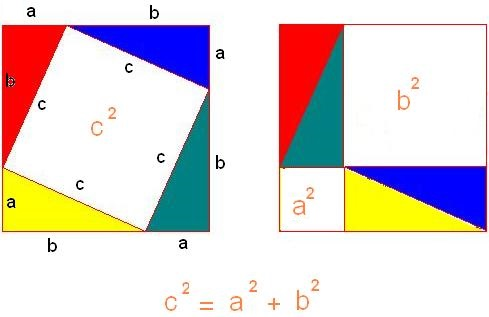
\includegraphics[scale=1]{images/01_precalculo/Pythagore.jpg}
\caption{Pitagoras}
\end{figure}

\begin{proof}
El área del cuadrado grande es 

$A = (a+b)(a+b) = a^2 + 2ab + b^2$

El área del cuadrado chico es $c^2$.  Pero además el área del cuadrado grande es igual a la del cuadrado chico mas cuatro veces el área del triángulo amarillo.  Es decir

$ a^2 + 2ab + b^2 = c^2 + 4 \frac{ab}{2} $

$ a^2 + 2ab + b^2 = c^2 + 2 ab $

$ a^2 + b^2 = c^2 $

como queríamos demostrar.
\end{proof}



\section{Números irracionales} \index{Conjunto!Números reales!Irracionales}

Veamos que algunos números reales no son racionales.  A los números reales que no son racionales los llamamos \textbf{irracionales}.

Supongamos que tenemos un cuadrado de lado 1 como en la figura.

\begin{figure}[h]
\centering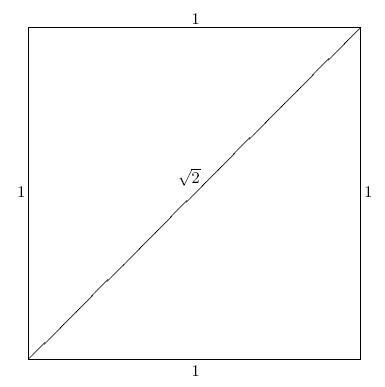
\includegraphics[scale=0.5]{images/01_precalculo/unit-square-with-diagonal.jpg}
\caption{Diagonal de un cuadrado}
\end{figure}

Queremos determinar el largo $c$ de su diagonal.  Por el teorema de pitágoras sabemos que $c^2 = 1^2 + 1^2 = 2$, es decir que $c = \sqrt{2}$.  

\begin{theorem}
$\sqrt{2} \not\in \QQ$
\end{theorem}

\begin{proof}
Supongamos que $\sqrt{2}$ es un número racional, es decir $\sqrt{2} = p/q$, con $p,q \in \mathbb{N}$ y coprimos, es decir $(p:q) = 1$, de forma que la fracción esté expresada en forma irreducible.

Elevando al cuadrado se tiene

$ \frac{p^2}{q^2} = 2$

$ p^2 = 2 q^2$

O sea que $p^2$ es par.  Por el teorema fundamental de la aritmética esto implica que $p$ es par.  O sea que $p = 2m$.  Luego

$ 4m^2 = 2q^2$

$ 2m^2 = q^2$

Con un razonamiento análogo al anterior vemos que $q$ es par.  Esto es absurdo pues $p$ y $q$ eran coprimos.  El absurdo provino de suponer que $\sqrt{2}$ es racional.  Por lo tanto $\sqrt{2}$ no es racional.
\end{proof}

\begin{problem}
Prueba gráfica de que $32.5 = 31.5$.  ¿Cómo es posible?
\end{problem}

\begin{figure}[h]
\centering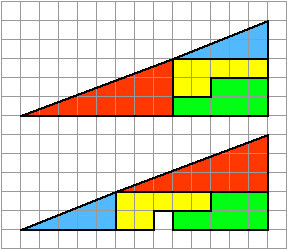
\includegraphics[scale=0.6]{images/01_precalculo/ilusion_triangulo.jpg}
\caption{Ilusión triángulo}
\end{figure}

Rta: Es una ilusión óptica.  El de arriba pareciera ser un triángulo de area $ \frac{13 \cdot 5}{2} = 32.5$.  Y el de abajo es reacomodar las fichas pero parece un triángulo con un cuadrado menos, es decir una region con área $31.5$.  

Pero en realidad ninguna de las dos figuras es un triángulo.  Basta ver que los ángulos de los triángulos rojo y azul no son iguales, sus tangentes (opuestos/adyancete) son $3/8 = 0.375 \neq 0.4 = 2/5 $.



\chapter{Polinomios}

\begin{definition}[Monomio] \index{Polinomio!Monomio}
Un \textbf{monomio} es una expresión en la que intervienen números reales, y variables, sólamente relacionadas por multiplicación (y potenciación con exponente natural).  

El \textbf{grado} del monomio es la suma de los exponentes de las variables.
\end{definition}

\begin{example}
Algunos monomios y sus grados:

\begin{itemize}
\item $12x^2y$ es de grado 3
\item $\pi z x^3$ es de grado 4
\item $-25 u^2$ es de grado 2
\end{itemize}
\end{example}

\begin{definition}[Polinomio] \index{Polinomio}
Un \textbf{polinomio} es una suma de monomios, y su \textbf{grado} es el grado del monomio de mayor \textbf{grado} que interviene en la suma.
\end{definition}

\begin{example}

Algunos polinomios y sus grados

\begin{itemize}
\item $12x^2y + \pi z x^3 $ es de grado 4
\item $3xy + z^2 - 3uv + x^3$ es de grado 3
\end{itemize}
	
\end{example}



\section{Polinomios en una indeterminada}

\begin{definition}[Polinomio en una variable] \index{Polinomio!Real}
En esta parte, sólamente vamos a trabajar con polinomios en una sóla variable ó indeterminada.  Al conjunto de todos los polinomios (con coeficientes en $\RR$) \textbf{en una sola variable} $x$ lo denotamos $\RR[x]$

Siempre podemos expresar un polinomio $p \in \RR[x]$ en la forma $p = \sum_{i=0}^n a_i x_i$, es decir

$$ p = a_0 + a_1 x + a_2 x^2 + \ldots + a_n x^n $$

con $a_n \neq 0$, y el grado del polinomio lo denotamos $gr(p) = n$

El polinomio nulo $p=0$ es el único polinomio que no tiene grado.

Decimos que el polinomio $p$ es \textbf{mónico} si $a_n = 1$.

Dos polinomios $p$  y $q$ son \textbf{iguales} si y sólo si sus coeficientes son iguales.  Es decir si $p = \sum_{i=0}^n a_i x^i$ y $q = \sum_{j=0}^m b_j x^j$ entonces $p=q$ si y sólo si $n=m$ y $a_i = b_i$ para todo $0 \leq i \leq n$
\end{definition}

\begin{example}
Algunos polinomios de $\RR[x]$
\begin{itemize}

\item $3x^2 + 2x -3$ es de grado 3
\item $\pi x + 8x^5 $ es de grado 5
\end{itemize}

\end{example}

\subsection{Operaciones con polinomios}

\begin{definition}[Suma y producto de polinomios] \index{Polinomio!Real!Suma y producto}
	
Sean $p = \sum_{i=0}^n a_i x^i$ y $q = \sum_{j=0}^m b_j x^j$.

Sea $r = max\{ n,m \}$

Entonces la \textbf{suma} la definimos como

$$ p+q = \sum_{k=0}^r (a_k+b_k) x^k $$

es decir se suma coeficiente a coeficiente.

El \textbf{producto} lo definimos como

$$ p \cdot q = \sum_{k=0}^{n+m} c_k x^k $$

donde 

$$ c_k = \sum_{i+j=k} a_i b_j $$

\end{definition}

\begin{observation}
Si $gr(p) = n$ y $gr(q) = m$ entonces $gr(pq) = n+m$
\end{observation}


\begin{definition}[Divisibilidad] \index{Polinomio!Real!Divisibilidad}
Si $p,q,r \in \mathbb{R}[x]$ y $p = qr$, decimos que $q$ \textbf{divide} a $p$, y lo denotamos $q|p$.
\end{definition}

\subsection{Algoritmo de división}

\begin{theorem}[Algoritmo de la división] \index{Polinomio!Real!Algoritmo de la división}
Si $p,q \in \mathbb{R}[x]$ entonces existen únicos polinomios $c,r$ tales que

$$ p = q \cdot c + r$$

con $r=0$ o $gr(r) < gr(q)$

Decimos que $p$ es el \textbf{dividendo}, $q$ el \textbf{divisor}, $c$ el \textbf{cociente}, y $r$ el \textbf{resto}.
\end{theorem}

\begin{definition}[Especialización] \index{Polinomio!Real!Especialización}
Sea $p \in \mathbb{R}[x]$, de forma $p = \sum_{i=0}^n$, y sea $\alpha \in \mathbb{R}$.  La \textbf{especialización} de $p$ en $\alpha$ es el número real

$$ p(\alpha) = \sum_{i=0}^n a_i \alpha^i $$
\end{definition}

\begin{definition}[Raíces y multiplicidad] \index{Polinomio!Real!Raíz y multiplicidad}

Si $p(\alpha) = 0$ se dice que $\alpha$ es una \textbf{raíz} (o un cero) de $p$.  

Decir que $\alpha \in \mathbb{R}$ es raíz de $p$ equivale a decir que $(x-\alpha)$ divide a $p$

Sea $\alpha \in \mathbb{R}$ raíz de $p \in \mathbb{R}[x]$, y sea $a \in \mathbb{N}$ tal que $(x-\alpha)^a | p$ pero $(x-\alpha)^{a+1} \not| p$.  Decimos que $a$ es la \textbf{multiplicidad} de $\alpha$ como raíz de $p$.

Si $a = 1$ se dice que $\alpha$ es \textbf{raíz simple} de $p$, sinó, $a>1$ y se dice que $\alpha$ es \textbf{raíz múltiple} de $p$.
\end{definition}


\begin{theorem}[del resto] \index{Polinomio!Real!Teorema del resto}
Sean $p, q \in \mathbb{R}[x]$, con $q = x - \alpha$.  El resto de dividir $p$ por $q$ es igual a $p(\alpha)$
\end{theorem}

\begin{proof}
Por el algoritmo de la división existen $c$ y $r$ tales que $p(x) = (x-\alpha) c(x) + r(x)$ con $gr(r) < gr(q) = 1$ o $r=0$.  Es decir $r$ constante.

Especializando en $\alpha$ obtenemos $p(\alpha) = r$.
\end{proof}

\begin{definition}[Polinomio irreducible] \index{Polinomio!Real!Irreducible}
Sea $p \in \mathbb{R}[x]$.  Decimos que $p$ es un polinomio \textbf{irreducible} si sus únicos divisores son los polinomios constantes y los polinomios de la forma $c \cdot p$ con $c$ constante.
\end{definition}

\begin{theorem}[Teorema Fundamental de la Aritmética para polinomios] \index{Polinomio!Real!TFA para polinomios}

Sea $p \in \mathbb{R}[x]$.  Entonces existen únicos $c \in \mathbb{R}$, polinomios irreducibles distintos $p_1, p_2, \ldots, p_n \in \mathbb{R}[x]$, y $a_1, a_2, \ldots, a_n \in \mathbb{N}$ de forma que

$$ p = c p_1^{a_1} p_2^{a_2} \ldots p_n^{a_n} $$

\end{theorem}

\begin{theorem}[Gauss] \index{Polinomio!Real!Teorema de Gauss}
Sea $P \in \mathbb{Z}[x]$, $p = a_0 + a_1x + a_2x^2 + \ldots + a_nx^n$, con $a_i \in \mathbb{Z}$ para $0 \leq i \leq n$, y $a_n \neq 0$.  Si $\alpha = \frac{p}{q} \in \mathbb{Q}$ es raíz de $P$, con $(p:q) = 1$, entonces $q | a_n$ y $p | a_0$.
\end{theorem}

\begin{proof}
Como $\alpha = p/q$ es raíz, se tiene que $P(p/q) = 0$, o sea

$a_0 + a_1 \frac{p}{q} + a_2 \frac{p^2}{q^2} + \ldots + a_{n-1} \frac{p^{n-1}}{q^{n-1}} + a_n \frac{p^n}{q^n} = 0$

multiplico por $q^n$

$a_0 q^n + a_1 p q^{n-1} + a_2 p^2 q^{n-2} + \ldots + a_{n-1} p^{n-1} q +  a_n p^n = 0$

saco factor común $p$

$a_0 q^n + p [a_1 q^{n-1} + a_2 p^1 q^{n-2} + \ldots + a_n p^{n-1}] = 0$

Como $p$ divide a $0$ y al segundo sumando, también divide a $a_0 q^n$, pero como $(p:q) = 1$ se tiene que $p | a_0$

Similarmente, sacando factor $q$

$q[a_0 q^{n-1} + a_1 p q^{n-2} + a_2 p^2 q^{n-3} + \ldots a_{n-1} p^{n-1}] + a_n p^n = 0$

Como $q$ divide a $0$ y al primer sumando, se tiene que $q$ divide a $a_n p^n$.  Pero como $(p:q) = 1$, se tiene que $q | a_n$.
\end{proof}

\begin{proposition}[Ecuación de primer grado] \index{Polinomio!Real!Ecuación lineal}
Una ecuación de \textbf{primer grado} (o \textbf{ecuación lineal}) es de la forma

$$ ax + b = 0 $$

con $a \neq 0$, y su única solución es $x = -b/a$.
\end{proposition}

\begin{proposition}[Ecuación de segundo grado] \index{Polinomio!Real!Ecuación cuadrática}
Una ecuación de \textbf{segundo grado} (o \textbf{ecuación cuadrática}) es de la forma

$$ ax^2 + bx + c = 0 $$

con $a \neq 0$.  Sus soluciones (en $\CC$) son dadas por la \textbf{fórmula resolvente}: \label{formula_resolvente}

$$ x_{1,2} = \frac{-b \pm \sqrt{b^2 - 4ac}}{2a}  $$

\end{proposition}

\begin{proof}
	
Divido por $a$

$ x^2 + \frac{b}{a}x + \frac{c}{a} = 0 $

completo cuadrado, es decir busco $\alpha, \beta \in \mathbb{R}$ tal que $(x-\alpha)^2 + \beta = x^2 + \frac{b}{a}x$, es decir

$ x^2 - 2\alpha x + \alpha^2 + \beta = x^2 + \frac{b}{a}x $

entonces resulta que $\alpha = \frac{-b}{2a}$ y $\beta = - \frac{b^2}{4a^2}$.  Luego

$ x^2 + \frac{b}{a}x + \frac{c}{a} = (x + \frac{b}{2a} )^2 - \frac{b^2}{4a^2} + \frac{c}{a}= 0 $

$(x + \frac{b}{2a} )^2 =  \frac{b^2}{4a^2} - \frac{c}{a} $

$(x + \frac{b}{2a} )^2 =  \frac{b^2}{4a^2} - \frac{4ac}{4a^2} $

$(x + \frac{b}{2a} )^2 =  \frac{b^2 - 4ac}{4a^2} $

Llamamos \textbf{discriminante} a $\triangle = b^2 - 4ac$

Debe darse uno de tres casos

\begin{itemize}

\item Si $\triangle > 0$, tenemos dos raíces reales y distintas

$ |x + \frac{b}{2a}| = \frac{\sqrt{ \triangle }}{2a}$

$$ x_{1,2} = \frac{-b}{2a} \pm \frac{\sqrt{ \triangle }}{2a} = \frac{-b \pm \sqrt{b^2 - 4ac}}{2a}$$

\item Si $\triangle = 0$, se tiene una sola raíz real doble.

$$ x = \frac{-b}{2a}$$

\item Si $\triangle < 0$, la ecuación no tiene raíces reales.  Se tienen dos raíces complejas conjugadas

$$x_{1,2} = \frac{-b \pm i \sqrt{4ac - b^2}}{2a}$$

\end{itemize}

En los tres casos se verifica

$$ x_{1,2} = \frac{-b \pm \sqrt{b^2 - 4ac}}{2a}  $$

\end{proof}




\chapter{Sistemas de ecuaciones lineales}

\begin{definition}[Sistema de ecuaciones] \index{Sistema de ecuaciones}
Un \textbf{sistema de ecuaciones} $Ax=k$ es una expresión de la forma

$$ S = \begin{cases}\begin{array}{lcl} 
a_{11} x_1 + a_{12} x_2 + \ldots + a_{1n} x_n & = & k_1 \\
a_{21} x_1 + a_{22} x_2 + \ldots + a_{2n} x_n & = & k_2 \\
& \ldots \\
a_{m1} x_1 + a_{m2} x_2 + \ldots + a_{mn} x_n & = & k_m
\end{array} \end{cases} $$

con $a_{ij} \in \mathbb{R}$ para $1 \leq i \leq m$, $1 \leq j \leq n$, y con $k_i \in \mathbb{R}$ para $1 \leq i \leq m$.

O dicho matricialmente $Ax = k$ con

$$ \underbrace{ \begin{pmatrix} 
a_{11} & a_{12} & \ldots & a_{1n} \\
a_{21} & a_{22} & \ldots & a_{2n} \\
\vdots & & & \\
a_{m1} & a_{m2} & \ldots & a_{mn} 
\end{pmatrix}}_A \underbrace{\begin{pmatrix} x_1 \\ x_2 \\ \vdots \\ x_n \end{pmatrix}}_x = \underbrace{ \begin{pmatrix} k_1 \\ k_2 \\ \vdots \\ k_m \end{pmatrix} }_k $$

La \textbf{matriz asociada} a dicho sistema es

$$ \begin{pmatrix} 
a_{11} & a_{12} & \ldots & a_{1n} & | & k_1 \\
a_{21} & a_{22} & \ldots & a_{2n} & | & k_2 \\
\vdots & & & & | & \\
a_{m1} & a_{m2} & \ldots & a_{mn} & | & k_m 
\end{pmatrix}$$

El \textbf{conjunto de soluciones} del sistema es $S = \{ x \in \RR^n : Ax = k \}$

Dos sistemas se dicen \textbf{equivalentes} si tienen el mismo conjunto de soluciones.  

\end{definition}

\begin{observation}[Operaciones elementales] \index{Sistema de ecuaciones!Operaciones elementales}
	
Siempre se puede llevar un sistema a otro equivalente realizando las siguientes \textbf{operaciones elementales}

\begin{itemize}
\item Permutar ecuaciones / permutar filas.
\item Multiplicar una ecuación/una fila por un escalar $\lambda \neq 0$.
\item A una fila sumarle un múltiplo de otra.
\end{itemize}

\end{observation}

\begin{definition}[Clasificación según soluciones] 
Dado un sistema $S$, entonces se da uno (y solo uno) de los siguientes casos:

\begin{itemize}
\item $\# S = 1$, se lo llama \textbf{Sistema Compatible Determinado} (SCD), y existe una única solución. \index{Sistema de ecuaciones!Clasificación!SCD}
\item $\# S > 1$, se lo llama \textbf{Sistema Compatible Indeterminado} (SCI), y existe más de una solución (y por lo tanto infinitas). \index{Sistema de ecuaciones!Clasificación!SCI}
\item $\# S = 0$, se lo llama \textbf{Sistema Incompatible} (SI), y no tiene ninguna solución. \index{Sistema de ecuaciones!Clasificación!SI}
\end{itemize}
\end{definition}

\subsection{Método de eliminación de Gauss} \index{Sistema de ecuaciones!Método de eliminación de Gauss}

Consiste en realizar las operaciones elementales hasta llevar el sistema a uno equivalente pero que sea triangular inferior, es decir de la forma

$$ \begin{pmatrix} 
a_{11} & a_{12} & \ldots & a_{1n} & | & k_1 \\
0 & a_{22} & \ldots & a_{2n} & | & k_2 \\
0 & 0 & \vdots & \vdots & | & \vdots \\
0 & 0 & 0 & a_{mn} & | & k_m 
\end{pmatrix}$$

Luego reemplazando de las últimas ecuaciones hacia las primeras encontramos todas las soluciones posibles, si es que existen.



\chapter{Funciones}

Recordar la definición de función (Ver \ref{funcion}).

\begin{definition}[Función real] \index{Función!Real}
Una función $f$ se dice que es una \textbf{función real} si es de la forma $f : A \to \mathbb{R}$.  

Un \textbf{cero} \index{Función!Real!Cero o raíz} (o raíz) de $f$ es un $x \in A$ tal que $f(x) = 0$.

Denotamos al conjunto de ceros (o \textbf{conjunto de nivel 0}) de $f$ como

$$ C_0(f) = \{x \in A / f(x) = 0 \} $$

\end{definition}

\begin{definition}[Operaciones con funciones reales] \index{Función!Real!Operaciones}

Sean $f, g : A \to \mathbb{R}$.  Entonces

\begin{itemize}
\item $f+g : A \to \mathbb{R}$ se define de forma tal que $(f+g)(x) = f(x) + g(x)$
\item $f-g : A \to \mathbb{R}$ se define de forma tal que $(f-g)(x) = f(x) - g(x)$
\item $f \cdot g : A \to \mathbb{R}$ se define de forma tal que $(f \cdot g)(x) = f(x) \cdot g(x)$
\item $f/g : A - C_0(g) \to \mathbb{R}$ se define de forma tal que $(f / g)(x) = f(x) / g(x)$
\end{itemize}
\end{definition}

\begin{definition}[Función par, impar, monótona] \index{Función!Real!Par, impar, monótona}

Sea $f : A \subseteq \mathbb{R} \to \mathbb{R}$, se dice que

\begin{itemize}
\item $f$ es \textbf{par} si $f(x) = f(-x)$ para todo $x \in A$.
\item $f$ es \textbf{impar} si $f(x) = -f(-x)$ para todo $x \in A$.
\item $f$ es \textbf{monótona estríctamente creciente} (o estríctamente creciente), si $x < y$ implica que $f(x) < f(y)$ para todo $x,y \in A$.
\item $f$ es \textbf{monótona estríctamente decreciente} (o estríctamente decreciente), si $x < y$ implica que $f(x) > f(y)$ para todo $x,y \in A$.

\end{itemize}

\end{definition}

\section{Ejemplos de funciones}

\begin{definition}[Función lineal] \index{Función!Ejemplos!Función lineal}

La \textbf{función lineal} es de la forma $f : \mathbb{R} \to \mathbb{R}$ con 

$$ f(x) = mx + b $$

con $m,b \in \mathbb{R}$.

Su gráfica representa una \textbf{recta} en el plano, a $m$ se lo llama \textbf{pendiente} de la recta.

Dos rectas de ecuaciones $y = m_1 x + b_1$ e $y = m_2 x + b_2$ se dicen \textbf{perpendiculares} (se cortan formando un ángulo de $90^{\circ}$) sólamente si 

$$\boxed{m_2 = \frac{-1}{m_1}}$$

\end{definition}

\begin{definition}[Función módulo] \index{Función!Ejemplos!Función módulo}

Recordamos que (ver \ref{funcion_modulo}) la \textbf{función valor absoluto} (o módulo) es $|\cdot| : \mathbb{R} \to \mathbb{R}$ con

$$|x| = \begin{cases} x & \textrm{ si } x \geq 0 \\ -x & \textrm{ si } x < 0 \end{cases}$$

$f(\mathbb{R}) = \mathbb{R}_0^+$
\end{definition}

\begin{definition}[Función signo] \index{Función!Ejemplos!Función signo}
La \textbf{función signo} es $sg : \mathbb{R} - \{0\} \to \mathbb{R}$ con

$$sg(x) = \begin{cases} 1 & \textrm{ si } x > 0 \\ -1 & \textrm{ si } x < 0 \end{cases}$$
\end{definition}

\begin{definition}[Función cuadrática] \index{Función!Ejemplos!Función cuadrática}
La \textbf{función cuadrática} es $f : \mathbb{R} \to \mathbb{R}$ con

$$f(x) = ax^2 + bx + c$$

con $a,b,c \in \mathbb{R}$, y $a \neq 0$.

Su gráfica es una parábola cuyo eje de simetría es paralelo al eje de ordenadas.  Dicho eje de simetría es $x = -b/2a$

Sus ceros pueden obtenerse utilizando la fórmula resolvente (ver \ref{formula_resolvente}).  Si $\triangle < 0$ la función no tiene ceros (reales).
\end{definition}

\begin{definition}[Función polinómica] \index{Función!Ejemplos!Función polinómica}
Una \textbf{función polinómica} es de la forma $f:\mathbb{R} \to \mathbb{R}$ con 

$$f(x) = a_n x^n + a_{n-1} x^{n-1} + \ldots + a_1 x + a_0 $$

con $a_i \in \mathbb{R}$ con $0 \leq i \leq n$.
\end{definition}

\begin{definition}[Función racional] \index{Función!Ejemplos!Función racional}
Una \textbf{función racional} es de la forma $f : \mathbb{R} - C_0(q(x)) \to \mathbb{R}$ con $f(x) = p(x)/q(x)$ sinedo $p(x)$ y $q(x)$ polinomios, y $C_0(q(x))$ el conjunto de ceros reales de $q(x)$.

Si $gr(q) = 1$ y $gr(p) \leq 1$ se denomina \textbf{función homográfica}, se expresa como

$$f(x) = \frac{ax+b}{cx+d}$$

con $c \neq 0$.

Tiene asíntota vertical $x = -d/c$, y asíntota horizontal $y = a/c$.

La imagen es $Im(f) = \mathbb{R} - \{ a/c \}$

Si $f(x) = kx$ se conoce como \textbf{variación directa}, con constante de proporcionalidad $k$.

Si $f(x) = \frac{k}{x}$ se conoce como \textbf{variación inversa}, con constante de proporcionalidad $k$.
\end{definition}

\section{Función compuesta}

\begin{definition} \index{Función!Compuesta}
Sea $f : A \to B$ y $g : C \to D$ con $B \subseteq C$.  Entonces podemos definir la \textbf{función compuesta} $g \circ f : A \to D$, donde 

$$(g \circ f)(x) = g(f(x))$$
\end{definition}

\section{Función inyectiva, sobreyectiva, biyectiva}

Una función $f : A \to B$ se dice \textbf{inyectiva} \index{Función!Inyectiva} sii $f(a) = f(b)$ implica que $a=b$.  Equivaléntemente si $a \neq b$ implica que $f(a) \neq f(b)$.

Una función $f : A \to B$ se dice \textbf{sobreyectiva} \index{Función!Sobreyectiva}, si $f(A) = B$.

Si una función $f : A \to B$ es inyectiva y sobreyectiva, decimos que es \textbf{biyectiva} \index{Función!Biyectiva}.  Esto equivale a decir que existe una \textbf{función inversa} \index{Función!Función inversa} $g : B \to A$ tal que $g(f(x)) = f(g(x)) = x$

\section{Funciones trascendentes}

\begin{definition}[Función exponencial] \index{Función!Ejemplos!Función exponencial}
Una \textbf{función exponencial} es una función de la forma $f : \mathbb{R} \to \mathbb{R}^+$ con $f(x) = a^x$ con $a \in (0,1) \cup (1, +\infty)$

\end{definition}

\begin{property}
Propiedades de la función exponencial

\begin{itemize}

\item No presenta ceros.

\item $ a^{x+y} = a^x a^y$ 

\item $a^{x-y} = a^x / a^y$

\item Si $a \in (0,1)$ la función es estríctamente decreciente, y si $a \in (1, +\infty)$  la función es estrictamente creciente.

\item La recta $y=0$ es la asíntota horizontal, y no tiene asíntota vertical.

\item Es biyectiva, es decir tiene inversa: la función logarítmica.

\end{itemize}
\end{property}

\begin{definition}[Función logarítmica] \index{Función!Ejemplos!Función logarítmica}

Llamamos \textbf{función logarítmica} de base $a \in (0,1) \cup (1, +\infty)$ a la inversa de la función exponencial de base $a$.  

Es decir $g : \mathbb{R}^+ \to \mathbb{R}$ con $g(x) = \log_a(x)$.

Es decir que se verifica que

$$ \log_a(a^x) = a^{\log_a(x)} = x $$
	
\end{definition}

\begin{property}

Propiedades de la función logarítmica

\begin{itemize}

\item Es una función biyectiva.

\item Tiene un único cero $x=1$.

\item La recta de ecuación $x=0$ es asíntota vertical, y no tiene asíntota horizontal.

\item $ \log_a(xy) = \log_a(x) + \log_a(y)$ (para todo $x,y > 0$)

\item $ \log_a(x/y) = \log_a(x) - \log_a(y)$ (para todo $x,y > 0$)

\item $ \log_a(x^y) = y \log_a(x)$ para todo $y \in \mathbb{R}$, $x > 0$

\item Si conocemos $\log_a(x)$ y queremos conocer $\log_b(x)$ con $b \neq a$, podemos aplicar la fórmula

$$ \log_b(x) = \frac{\log_a(x)}{\log_a(b)}$$

que demostramos a continuación

$ y = \log_b(x)$

$ b^y = x $

$ \log_a(b^y) = \log_a(x) $

$ y \log_a(b) = \log_a(x) $

$ y = \frac{\log_a(x)}{\log_a(b)} $

$ \log_b(x) = \frac{\log_a(x)}{\log_a(b)} $
\end{itemize}
\end{property}



\chapter{Trigonometría}

\begin{definition}[Definiciones básicas] \index{Trigonometría}

Llamamos \textbf{plano euclídeo} al conjunto

$$ \mathbb{R}^2 = \{ (x,y) : x, y \in \mathbb{R} \} $$

cuyos elementos llamamos puntos o vectores, con las siguientes operaciones.

Sean $(x_1,x_2)$ e $(y_1,y_2)$ dos vectores.

La \textbf{suma} es $(x_1+y_1, x_2+y_2)$.  

Sea $\lambda \in \mathbb{R}$, entonces el \textbf{producto de un vector por un escalar} es $\lambda(x_1,x_2) = (\lambda x_1, \lambda x_2)$

El producto interno estándard (o \textbf{producto escalar}) es

$$ (x_1,x_2) \cdot (y_1,y_2) = x_1 y_1 + x_2 y_2 $$

La \textbf{norma} de un vector $(x_1, x_2)$ se define como

$$ ||(x_1,x_2)|| = \sqrt{ (x_1, x_2) \cdot (x_1,x_2) } = \sqrt{x_1^2 + x_2^2} $$

La \textbf{distancia} entre dos puntos $(x_1,x_2)$ e $(y_1,y_2)$ se define como

$$ d((x_1,x_2), (y_1,y_2)) = ||(x_1,x_2) - (y_1,y_2) || = \sqrt{(x_1-y_1)^2 + (x_2-y_2)^2} $$

La \textbf{circunferencia unitaria} $C$ es el conjunto de puntos que dista 1 del origen de coordenadas, es decir son los $(x,y) \in \mathbb{R}^2$ tales que

$$ d((x,y),(0,0)) = 1 $$

$$ \sqrt{(x-0)^2 + (y-0)^2} = 1 $$

$$ x^2 + y^2 = 1 $$

Dado un punto $(x,y) \in C$, el mismo forma cierto \textbf{ángulo} $\phi$ con el eje $x$.  Dicho ángulo $\phi$ puede medirse en distintas unidades, como grados, o radianes.  

En este apunte vamos a asumir que utilizamos siempre \textbf{radianes}, que equivale a la longitud del segmento de circunferencia unitaria correspondiente.  En particular un giro completo equivale a $2\pi$.

\end{definition}

\begin{figure}[h]
\centering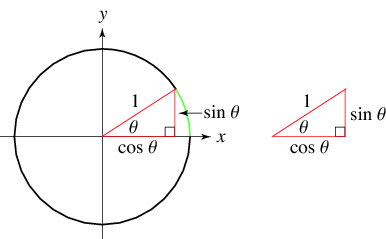
\includegraphics[scale=0.5]{images/01_precalculo/trigonometry.png}
\caption{Trigonometría}
\end{figure}

\begin{figure}[h]
\centering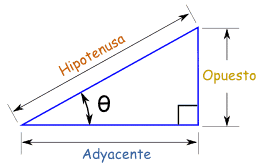
\includegraphics[scale=0.6]{images/01_precalculo/hipotenusa.png}
\caption{Hipotenusa}
\end{figure}

\begin{definition}
Definimos las \textbf{funciones trigonométricas} $\cos(\phi) = x$ y $\sin(\phi) = y$, llamadas coseno de $\phi$ y seno de $\phi$ respectivamente.

En la siguiente figura podemos ver la circunferencia unitaria y un ángulo $\theta$ en verde.  Vemos que queda formado un triángulo rectángulo en rojo.


En términos de un triángulo rectángulo, llamamos \textbf{catetos} a los lados del ángulo rectángulo, e hipotenusa al otro lado.  En términos del ángulo $\phi$ entre la hipotenusa y un cateto, lo llamamos \textbf{cateto adyacente}, y al otro cateto lo llamamos \textbf{cateto opuesto}.

Se verifica entonces

$$\cos(\theta) = \frac{\textrm{Adyacente}}{\textrm{Hipotenusa}}$$

$$\sin(\theta) = \frac{\textrm{Opuesto}}{\textrm{Hipotenusa}}$$

Definimos también las \textbf{funciones trigonométricas} tangente, secante, cosecante y cotangente a continuación, siempre y cuando no se anule el denominador.

$$ \tan(\theta) = \frac{\sin(\theta)}{\cos(\theta)}$$

$$ \sec(\theta) = \frac{1}{\cos(\theta)}$$

$$ \mathrm{cosec}(\theta) = \frac{1}{\sin(\theta)}$$

$$ \cot(\theta) = \frac{1}{\tan(\theta)}$$

\end{definition}

\begin{observation}[Identidad trigonométrica fundamental] \index{Trigonometría!Identidad trigonométrica fundamental}
Para cualquier $\phi \in \mathbb{R}$ se verifica la identidad trigonométrica fundamental:

$$ \cos^2(\phi) + \sin^2(\phi) = 1$$
\end{observation}

\begin{proof}
Dado $\phi \in \RR$, como $x = \cos(\phi)$, $y = \sin(\phi)$ y $(x,y)$ es un punto de la circunferencia unitaria $x^2 + y^2 = 1$, se verifica $\cos^2(\phi) + \sin^2(\phi) = 1$.
\end{proof}



\section{Tabla de ángulos y valores} \index{Trigonometría!Tabla de ángulos y valores}

Puede ser útil conocer los siguientes datos sobre algunos ángulos.

\begin{figure}[h]
\centering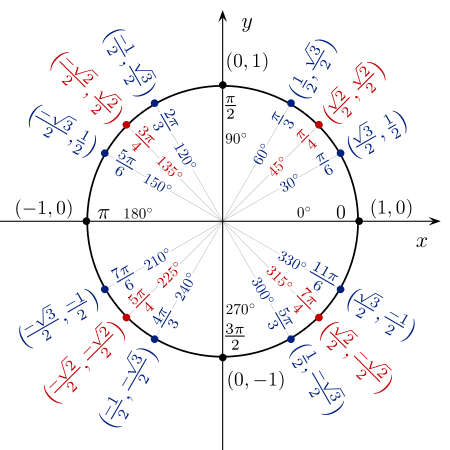
\includegraphics[scale=0.5]{images/01_precalculo/unit_circle_angles_color.png}
\caption{Ángulos en la circunferencia unitaria}
\end{figure}

\begin{center}
  \begin{tabular}{| c | c | c | c | }
    \hline
    Radianes & Grados & Vértice & Aproximado \\ \hline \hline
    $0$ & $0$ & $(1,0)$ & $(1,0)$ \\ 
    $\pi/6$ & $30$ & $(\sqrt{3}, 1)/2$ & $(0.866, 0.5)$ \\
    $\pi/4$ & $45$ & $(\sqrt{2}, \sqrt{2})/2$ & ($0.707, 0.707)$ \\
    $\pi/3$ & $60$ & $(1, \sqrt{3})/2$ & $(0.5, 0.866)$ \\
    $\pi/2$ & $90$ & $(0, 1)$ & $(0, 1)$ \\
    $2\pi/3$ & $120$ & $(-1, \sqrt{3})/2$ & $(-0.5, 0.866)$ \\
    $3\pi/4$ & $135$ & $(-\sqrt{2}, \sqrt{2})/2$ & $(-0.707, 0.707)$ \\
    $5\pi/6$ & $150$ & $(-\sqrt{3}, 1)/2$ & $(-0.866, 0.5)$ \\
    $\pi$ & $180$ & $(-1, 0)$ & $(-1, 0)$ \\
    $7\pi/6$ & $210$ & $(-\sqrt{3}, -1)/2$ & $(-0.866, -0.5)$ \\
    $5\pi/4$ & $225$ & $(-\sqrt{2}, -\sqrt{2})/2$ & $(-0.707, -0.707)$ \\
    $4\pi/3$ & $240$ & $(-1, -\sqrt{3})/2$ & $(-0.5, -0.866)$ \\
    $3\pi/2$ & $270$ & $(0, -1)$ & $(0, -1)$ \\
    $5\pi/3$ & $300$ & $(1, -\sqrt{3})/2$ & $(0.5, -0.866)$ \\
    $7\pi/4$ & $315$ & $(\sqrt{2}, -\sqrt{2})/2$ & $(0.707, -0.707)$ \\
    $11\pi/6$ & $330$ & $(\sqrt{3}, -1)/2$ & $(0.866, -0.5)$ \\
    $2\pi$ & $0$ & $(1,0)$ & $(1,0)$ \\ 

    \hline
  \end{tabular}
\end{center}


\section{Funciones trigonométricas}

\begin{definition}[Seno] \index{Trigonometría!Función $\sin(x)$ }
La \textbf{función seno} es $\sin : \mathbb{R} \to \mathbb{R}$ con 

$$ x \to \sin(x)$$

A continuación la \textbf{gráfica} de la función seno
\end{definition}

\begin{figure}[h]
\centering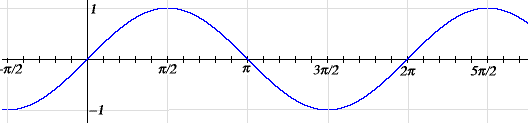
\includegraphics[scale=0.5]{images/01_precalculo/sin.png}
\caption{$\sin(x)$}
\end{figure}

\begin{property}
Algunas propiedades de $\sin(x)$

\begin{itemize}
	
\item Sus \textbf{ceros} son $C_0(f) = \{ k\pi, \textrm{ con } k \in \mathbb{Z} \}$
	
\item Es \textbf{impar}, es decir $\sin(-x) = -\sin(x)$
	
\end{itemize}
\end{property}

\begin{definition}[Coseno] \index{Trigonometría!Función $\cos(x)$ }
La \textbf{función coseno} es $\cos : \mathbb{R} \to \mathbb{R}$ con 

$$ x \to \cos(x)$$

A continuación la gráfica de la función coseno.
\end{definition}

\begin{figure}[h]
\centering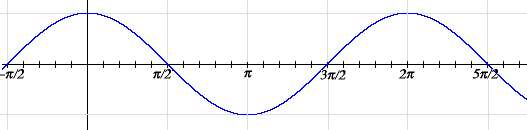
\includegraphics[scale=0.5]{images/01_precalculo/cos.png}
\caption{$\cos(x)$}
\end{figure}

\begin{property}
Algunas propiedades de $\cos(x)$

\begin{itemize}

\item Para todo ángulo se verifica que $\cos(x) = \sin(x + \frac{\pi}{2})$.  Es decir la curva se \textbf{traslada} en $\pi/2$ hacia la izquierda de la gráfica del seno.

\item Sus \textbf{ceros} son 

$$C_0(f) = \{ \frac{\pi}{2} + k\pi, \textrm{ con } k \in \mathbb{Z} \}$$

(son los de la función seno trasladados).

\item Es \textbf{par}, es decir $\cos(x) = \cos(-x)$

\end{itemize}
\end{property}

\begin{property}
Algunas propiedades comunes de $\sin(x)$ y $\cos(x)$

\begin{itemize}
\item La \textbf{imagen} tanto de $\sin(x)$ como de $\cos(x)$ es el intervalo $[-1,1]$.
	
\item Son \textbf{periódicas} con período $2\pi$, es decir $f(x) = f(x + 2\pi)$.  
	
O sea que el gráfico obtenido en el intervalo $[0, 2\pi)$ se repite periódicamente.
	
\item \textbf{No son inyectivas}.
\end{itemize}
\end{property}

\begin{definition}[Tangente] \index{Trigonometría!Función $\tan(x)$ }
La \textbf{función tangente} es $\tan : \mathbb{R} - C_0(\cos(x)) \to \mathbb{R}$, con 

$$ x \to \frac{\sin(x)}{\cos(x)} $$

A continuación su gráfica 
\end{definition}

\begin{figure}[h]
\centering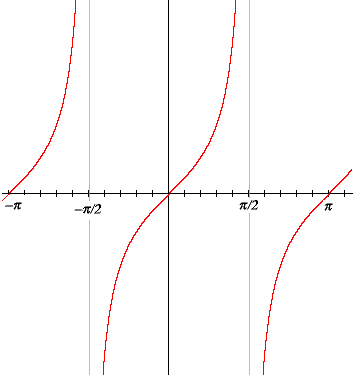
\includegraphics[scale=0.5]{images/01_precalculo/tan.png}
\caption{$\tan(x)$}
\end{figure}

\begin{property}
Algunas propiedades de $\tan(x)$

\begin{itemize}
\item Los \textbf{ceros} de $\tan(x)$ coinciden con los de $\sin(x)$
	
\item Es \textbf{impar}, es decir $\tan(-x) = -\tan(x)$
	
\item Es \textbf{periódica} con período $\pi$.  Es decir $\tan(x) = \tan(x+\pi)$.
	
\item Tiene \textbf{asíntotas verticales} $x = \frac{\pi}{2} + k \pi$ con $k \in \mathbb{Z}$
\end{itemize}
\end{property}

\subsection{Las funciones $\sec(x)$ y $\mathrm{cosec}(x)$ y $\cot(x)$}

\begin{definition}[Secante, cosecante y cotangente] 
La \textbf{función secante} \index{Trigonometría!Función Secante} $\sec : \mathbb{R} - C_0(\sin(x)) \to \mathbb{R}$ con $x \to \frac{1}{\cos(x)} $ 

A continuación su gráfica

La \textbf{función cosecante} \index{Trigonometría!Función Cosecante} $\mathrm{cosec}(x) = \frac{1}{\sin(x)}$ es análoga a la función secante.

La \textbf{función cotangente} \index{Trigonometría!Función Cotangente} es $\cot(x) = \frac{1}{\tan(x)}$.  A continuación su gráfica
\end{definition}

\begin{figure}[h]
\centering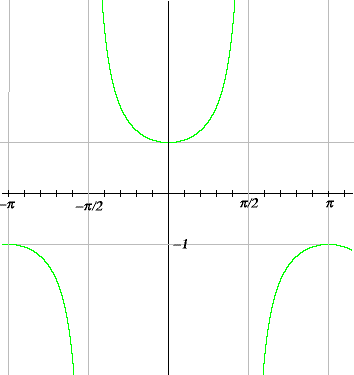
\includegraphics[scale=0.5]{images/01_precalculo/sec.png}
\caption{$\sec(x)$}
\end{figure}

\begin{figure}[h]
\centering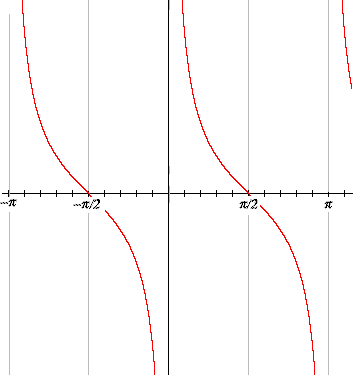
\includegraphics[scale=0.5]{images/01_precalculo/cot.png}
\caption{$\cot(x)$}
\end{figure}


\section{Funciones trigonométricas inversas}

Vimos que las funciones $\sin(x)$, $\cos(x)$ y $\tan(x)$ no son inyectivas.  

Restringiendo el dominio y el codominio podemos obtener una función biyectiva.

\begin{definition}
\begin{itemize}
Definimos las funciones trigonométricas inversas como sigue

\item Restringiendo $\sin(x)$ a $[-\frac{\pi}{2}, \frac{\pi}{2}] \to [-1,1]$ obtenemos una función biyectiva cuya inversa llamamos $ \arcsin(x) $. \index{Trigonometría!Función Arco-seno}

\item Restringiendo $\cos(x)$ a $[0, \pi] \to [-1,1]$ obtenemos una función biyectiva cuya inversa llamamos $ \arccos(x) $. \index{Trigonometría!Función Arco-coseno}

\item Restringiendo $\tan(x)$ a $(-\frac{\pi}{2}, \frac{\pi}{2}) \to \mathbb{R}$ obtenemos una función biyectiva cuya inversa llamamos $\arctan(x)$ \index{Trigonometría!Función Arco-tangente}

\end{itemize}
\end{definition}

\subsection{Ángulo respecto al eje $x$}

En el plano coordenado $\mathbb{R}^2$, es estandard medir ángulos respecto al lado positivo del eje $x$ en sentido antihorario, como muestra la figura

\begin{figure}[h]
\centering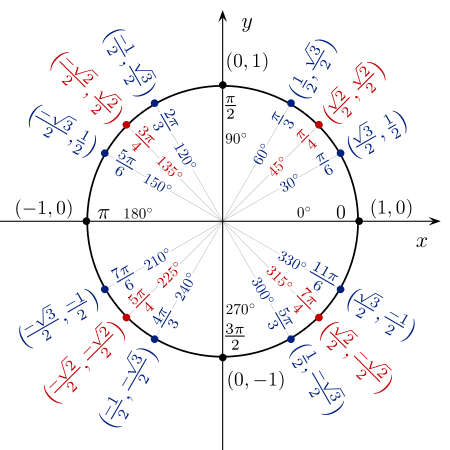
\includegraphics[scale=0.5]{images/01_precalculo/unit_circle_angles_color.png}
\caption{Ángulos en la circunferencia unitaria}
\end{figure}

Supongamos que queremos averiguar el ángulo que forma el vector $v = (-1,-1)$ respecto al eje $x$.  

Como $||v|| = \sqrt{2}$, sabemos que $\cos(\phi) = \sin(\phi) = - \sqrt{2}/2$

Ahora que pasa, la calculadora arroja los siguientes resultados: $\arccos(-\sqrt{2}/2) = 3 \pi/4 $ y $\arcsin(- \sqrt{2}/2) = - \pi / 4$.  

No sólo nos da dos resultados distintos entre sí, sino que ninguno de ellos es el buscado.  Notar que $3\pi/4$ pertenece al segundo cuadrante, $- \pi/4$ pertenece al cuarto cuadrante, y nuestro vector $(-1,-1)$ pertenece al tercer cuadrante.

La idea para obtener el ángulo correcto es analizar el cuadrante que queremos en el dibujo, y considerar ángulos semejantes en el cuadrante en cuestión.  En este caso queremos tercer cuadrante, y lo podemos obtener como $\pi + \pi/4 = 5\pi/4$

Ejercicio: Calcular el ángulo con respecto al eje $x$ de $(- \sqrt{3}, -1)$.  La respuesta es $7\pi/6 = 210^{\circ}$

\section{Función sinusoidal}

\begin{definition}[Función sinusoidal] \index{Función!Ejemplos!Función sinusoidal}
Una función $f$ se dice que es una \textbf{función sinusoidal} si es de la forma $f : \mathbb{R} \to \mathbb{R}$ con 

$$f(x) = K \sin(ax+b)$$

La curva gráfica de la función sinusoidal se llama onda sinusoidal, o sinusoide.  En el gráfico a continuación se representa una sinusoide.

\begin{itemize}
\item La \textbf{amplitud} es $\boxed{ K } $.

\item La \textbf{frecuencia} (ordinaria) es $ \boxed{f = \frac{a}{2\pi} }$ (cíclos por unidad de tiempo).

\item El \textbf{período} es $ \boxed{ \frac{1}{f} }$, el intervalo en que vuelve a empezar

\item La frecuencia angular es $a$.
\item La fase es $b$.
\item El ángulo de fase es $\frac{b}{a}$.  La curva se traslada en esa cantidad.

Si es negativo se retrasa, es decir se corre a la derecha.  Si es positivo se adelanta, es decir se corre a la izquierda.

\end{itemize}

Observar que la función coseno es sinusoidal porque $\cos(x) = \sin(x + \pi/2)$
\end{definition}

\begin{figure}[h]
\centering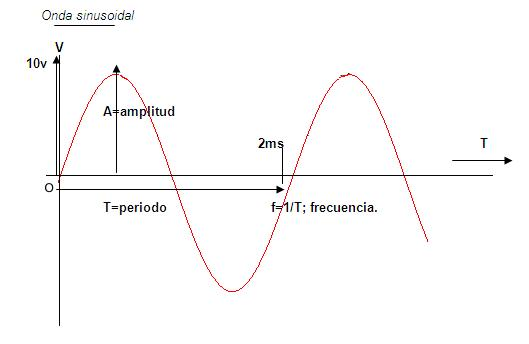
\includegraphics[scale=0.7]{images/01_precalculo/sinusoide.jpg}
\caption{Sinusoide}
\end{figure}

\section{Identidades trigonométricas}

\begin{definition}[Identidad trigonométrica] \index{Trigonometría!Identidad trigonométrica}
Una \textbf{identidad trigonométrica} es una ecuación que se verifican para todo valor del ángulo, por ejemplo la identidad trigonométrica fundamental 

$$ \cos^2(\phi) + \sin^2(\phi) = 1 $$
\end{definition}

\begin{definition}[Fórmula de Euler]
La \textbf{fórmula de Euler} establece que dado $\phi \in \mathbb{R}$, entonces

$$ e^{i \phi} = \cos(\phi) + i \sin(\phi) $$
\end{definition}

\begin{observation}
La exponencial compleja cumple la siguiente propiedad 

$$ e^{i (\alpha + \beta)} = e^{i \alpha} e^{i \beta} $$

Por lo tanto

\begin{eqnarray*} 
	e^{i (\alpha + \beta)} &=& \cos(\alpha + \beta) + i \sin(\alpha + \beta) \\
	&=& [\cos(\alpha) + i \sin(\alpha) ] [\cos(\beta) + i \sin(\beta)] \\
	&=& [\cos(\alpha)\cos(\beta) - \sin(\alpha)\sin(\beta)] + i [\cos(\alpha)\sin(\beta) + \sin(\alpha)\cos(\beta)]
\end{eqnarray*}
	
\end{observation}

\subsection{Suma de ángulos} 

Igualando parte real e imaginaria del número complejo obtenemos fórmulas para el seno y el coseno de la suma de dos ángulos:

\index{Trigonometría!Identidad trigonométrica!$\cos(\alpha + \beta)$ } \index{Trigonometría!Identidad trigonométrica!$\sin(\alpha + \beta)$ }

\begin{eqnarray*}
\cos(\alpha + \beta) &=& \cos(\alpha)\cos(\beta) - \sin(\alpha)\sin(\beta) \\
\sin(\alpha + \beta) &=& \cos(\alpha)\sin(\beta) + \sin(\alpha)\cos(\beta)
\end{eqnarray*}

También podemos verificar dichas identidades geométricamente mediante el siguiente gráfico 

\begin{figure}[h]
\centering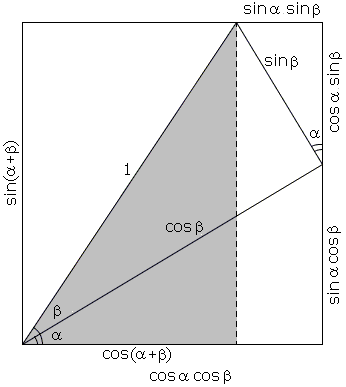
\includegraphics[scale=0.7]{images/01_precalculo/cos_of_sum.png}
\caption{Coseno de la suma}
\end{figure}

Y recordando que $\cos(x)$ es par, y $\sin(x)$ es impar, obtenemos fórmulas para el seno y el coseno de la diferencia de dos ángulos:

\index{Trigonometría!Identidad trigonométrica!$\cos(\alpha - \beta)$ } \index{Trigonometría!Identidad trigonométrica!$\sin(\alpha - \beta)$ }

\begin{eqnarray*}
\cos(\alpha - \beta) &=& \cos(\alpha)\cos(\beta) + \sin(\alpha)\sin(\beta) \\
\sin(\alpha - \beta) &=& \sin(\alpha)\cos(\beta) -\cos(\alpha)\sin(\beta)
\end{eqnarray*}

Además, para la tangente de la suma de dos ángulos obtenemos

\index{Trigonometría!Identidad trigonométrica!$\tan(\alpha + \beta)$ } 

\begin{eqnarray*}
\tan(\alpha + \beta) &=& \frac{\sin(\alpha + \beta)}{\cos(\alpha + \beta)} \\
 &=& \frac{\cos(\alpha)\sin(\beta) + \sin(\alpha)\cos(\beta)}{\cos(\alpha)\cos(\beta) - \sin(\alpha)\sin(\beta)} \\
 &=& \frac{\frac{\cos(\alpha)\sin(\beta)}{\cos(\alpha)\cos(\beta)} + \frac{\sin(\alpha)\cos(\beta)}{\cos(\alpha)\cos(\beta)}}{\frac{\cos(\alpha)\cos(\beta)}{\cos(\alpha)\cos(\beta)} - \frac{\sin(\alpha)\sin(\beta)}{\cos(\alpha)\cos(\beta)}} \\
 &=& \frac{\tan(\beta) + \tan(\alpha)}{1 - \tan(\alpha)\tan(\beta)}
\end{eqnarray*}

\subsection{Suma de senos y de cosenos}

Se verifica entonces que

\begin{eqnarray*}
\cos(\alpha + \beta) + \cos(\alpha - \beta) &=& 2 \cos(\alpha)\cos(\beta) \\
\cos(\alpha + \beta) - \cos(\alpha - \beta) &=& -2 \sin(\alpha) \sin(\beta) \\
\sin(\alpha + \beta) + \sin(\alpha - \beta) &=& 2 \sin(\alpha) \cos(\beta) \\
\sin(\alpha + \beta) - \sin(\alpha - \beta) &=& 2 \cos(\alpha) \sin(\beta) 
\end{eqnarray*}

Si $a = \alpha + \beta$ y $b = \alpha - \beta$, se tiene que $\alpha = \frac{a+b}{2}$ y $\beta = \frac{a-b}{2}$, y 

\index{Trigonometría!Identidad trigonométrica!$\cos(a) + \cos(b)$} 
\index{Trigonometría!Identidad trigonométrica!$\cos(a) - \cos(b)$} 
\index{Trigonometría!Identidad trigonométrica!$\sin(a) + \sin(b)$} 
\index{Trigonometría!Identidad trigonométrica!$\sin(a) - \sin(b)$} 

\begin{eqnarray*}
\cos(a) + \cos(b) &=& 2 \cos(\frac{a+b}{2})\cos(\frac{a-b}{2}) \\
\cos(a) - \cos(b) &=& -2 \sin(\frac{a+b}{2})\sin(\frac{a-b}{2}) \\
\sin(a) + \sin(b) &=& 2 \sin(\frac{a+b}{2}) \cos(\frac{a-b}{2}) \\
\sin(a) - \sin(b) &=& 2 \cos(\frac{a+b}{2}) \sin(\frac{a-b}{2}) 
\end{eqnarray*}

\subsection{Algo extra...}

Usando la fórmula de Euler, y que coseno es par y seno es par

\begin{eqnarray*}
e^{i \alpha} &=& \cos(\alpha) + i \sin(\alpha) \\
e^{- i \alpha} &=& \cos(\alpha) - i \sin(\alpha)
\end{eqnarray*}

Sumando y restando respectivamente

\begin{eqnarray*}
e^{i \alpha} + e^{-i \alpha} &=& 2 \cos(\alpha) \\
e^{i \alpha} - e^{-i \alpha} &=& 2 i \sin(\alpha)
\end{eqnarray*}

Por lo tanto

\begin{eqnarray*}
\cos(\alpha) &=& \frac{e^{i \alpha} + e^{-i \alpha}}{2} \\
\sin(\alpha) &=& \frac{e^{i \alpha} - e^{-i \alpha}}{2i}
\end{eqnarray*}

\section{Pendiente de una recta} \index{Trigonometría!Pendiente de una recta}

\begin{observation}[Pendiente de una recta]
La \textbf{ecuación cartesiana} de una recta $R$ en el plano es de la forma

$$ y = mx + b$$

Decimos que $m$ es la \textbf{pendiente} de la recta, y que $b$ es la \textbf{ordenada al origen}.

Entonces la pendiente $m$ de la recta $R$ es igual a la tangente del ángulo $\phi$ entre el eje $x$ y la recta dada.
\end{observation}

\begin{figure}[h]
\centering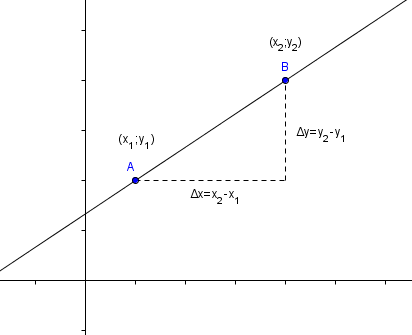
\includegraphics[scale=1]{images/01_precalculo/pendiente_recta.png}
\caption{Pendiente de una recta}
\end{figure}

\begin{proof}
Supongamos que sólo conocemos dos puntos de la recta $(x_1, y_1)$ y $(x_2, y_2)$, con $x_1 \neq x_2$, como se muestra en la siguiente figura, y que queremos encontrar la ecuación cartesiana de la recta.

Se tiene que una \textbf{ecuación paramétrica} de la recta $R$ es

$$(x,y) = (x_1, y_1) + \lambda(x_2 - x_1, y_2 - y_1)$$

con $\lambda \in \mathbb{R}$.  O sea que

\begin{eqnarray*}
x &=& x_1 + \lambda (x_2 - x_1) \\
y &=& y_1 + \lambda (y_2 - y_1) 
\end{eqnarray*}

De la primera ecuación

$$ \lambda = \frac{x - x_1}{x_2 - x_1}$$

En la segunda, y llamando $\triangle x = x_2 - x_1$ y $\triangle y = y_2 - y_1$

\begin{eqnarray*}
y &=& y_1 + \frac{x - x_1}{x_2 - x_1} (y_2 - y_1) \\
y &=& \frac{\triangle y}{\triangle x} x + \left( y_1 - x_1 \frac{\triangle y}{\triangle x} \right)
\end{eqnarray*}

Finalmente encontramos la ecuación cartesiana de la recta

$$ y = mx + b $$

donde $m = \frac{\triangle y}{\triangle x}$ y $ b = \left( y_1 - x_1 \frac{\triangle y}{\triangle x} \right) $

Notar que también podemos escribir esta ecuación como

$$ y - y_1 = m (x - x_1) $$

Volviendo a ver el dibujo, observamos que podemos formar un triángulo rectángulo donde $\triangle x$ y $\triangle y$ son sus catetos.  Considerando el ángulo $\alpha$ entre la recta $y = y_1$ y la recta dada, vemos que $m = \frac{\triangle y}{ \triangle x} = \tan(\alpha)$, pues es el cociente del cateto opuesto con el cateto adyacente.

Es decir que la pendiente de la recta es igual a la tangente del ángulo $\alpha$ entre la recta $R$ y la recta horizontal $y = y_1$.  O lo que es lo mismo, entre la recta $R$ y el eje $x$ (es el mismo ángulo $\alpha$).

\end{proof}

\section{Teoremas del seno y del coseno}

\begin{theorem}[Teorema del Seno] \label{teorema_del_seno}

Sea $ABC$ un triángulo, llamamos $\alpha, \beta, \gamma$ a sus ángulos, y $a,b,c$ a sus lados opuestos.

Entonces,

$$ \boxed{ \frac{a}{\sin(\alpha)} = \frac{b}{\sin(\beta)} = \frac{c}{\sin(\gamma)} } $$

\end{theorem}

\begin{figure}[h]
\centering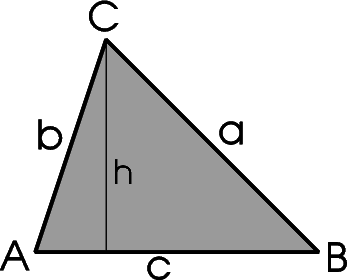
\includegraphics[scale=0.4]{images/01_precalculo/teorema_seno.png}
\caption{Teorema del seno}
\end{figure}

\begin{proof}
Si $h = b \sin(\alpha)$ es la altura desde el vértice $C$, entonces el área del triángulo es $A = \frac{ch}{2} = \frac{c b \sin(\alpha)}{2}$

Similarmente, trazando la altura desde los otros vértices obtenemos $A = \frac{ac \sin(\beta)}{2} = \frac{ab \sin(\gamma)}{2}$, es decir

$$ 2A = bc \sin(\alpha) = ac \sin(\beta) = ab \sin(\gamma) $$

dividiendo por $abc$

$$ \frac{2A}{abc} = \frac{\sin(\alpha)}{a} = \frac{\sin(\beta)}{b} = \frac{\sin(\gamma)}{c} $$

tomando el recíproco

$$ \frac{abc}{2A} = \frac{a}{\sin(\alpha)} = \frac{b}{\sin(\beta)} = \frac{c}{\sin(\gamma)} $$
\end{proof}

\begin{proof}
Ahora vamos a dar otra demostración, suponiendo que el triángulo es agudo.

Primero partimos el triángulo en dos triángulos rectángulos, trazando la altura $h$ desde el vértice $C$, como en la figura siguiente


Luego,

$$ h = b \sin(\alpha) = a \sin(\beta) $$

de donde

$$ \frac{a}{\sin(\alpha)} = \frac{b}{\sin(\beta)} $$

Si trazamos la altura desde el vértice $B$ obtenemos

$$ \frac{a}{\sin(\alpha)} = \frac{c}{\sin(\gamma)} $$

Finalmente

$$ \frac{a}{\sin(\alpha)} = \frac{b}{\sin(\beta)} = \frac{c}{\sin(\gamma)}$$

\end{proof}

\begin{theorem}[Teorema del Coseno] \label{teorema_del_coseno}

Sea $ABC$ un triángulo, llamamos $\alpha, \beta, \gamma$ a sus ángulos, y $a,b,c$ a sus lados opuestos.

Entonces,

$$ \boxed{a^2 = b^2 + c^2 - 2bc \cos(\alpha)} $$

y vale simétricamente para los otros lados, es decir

\begin{eqnarray*}
a^2 &=& b^2 + c^2 - 2bc \cos(\alpha) \\
b^2 &=& a^2 + c^2 - 2ac \cos(\beta) \\
c^2 &=& a^2 + b^2 - 2ab \cos(\gamma)
\end{eqnarray*}
\end{theorem}

\begin{figure}[h]
\centering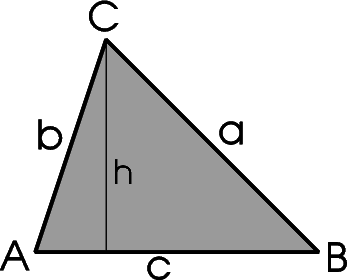
\includegraphics[scale=0.4]{images/01_precalculo/teorema_seno.png}
\caption{Teorema del coseno}
\end{figure}

Observación: En el caso particular de que el triángulo sea rectángulo nos queda el teorema de Pitágoras.  Es decir este teorema es una generalización del teorema de Pitágoras.

\begin{proof}  Demostramos utilizando producto interno.

Situamos el vértice de ángulo $\alpha$ en el origen del plano euclídeo.  Los lados $b$ y $c$ los interpretamos como vectores de $\mathbb{R}^2$, y al lado $a$ como el vector $c-b$.  Luego

$ ||a||^2 = || c-b ||^2 = (c-b) \cdot (c-b) = c^2 - 2bc + b^2 = ||c||^2 + ||b||^2 - 2 ||b|| ||c|| \cos(\alpha) $

Es decir que

$$a^2 = b^2 + c^2 - 2 bc \cos(\alpha)$$

\end{proof}

\begin{proof}  Demostramos utilizando distancia euclídea.
	
Dispongamos sus vértices en el plano cartesiano de la siguiente manera

$A = (0,0)$, $B = (b, 0)$ y $C = (a \cos(\alpha), a \sin(\alpha))$

La distancia entre $B$ y $C$ es 

$$ d(B,C) = c = \sqrt{(a \cos(\alpha) - b)^2 + (a \sin(\alpha) - 0)^2 } $$

Por lo tanto

$$ c^2 = a^2 \cos^2(\alpha) - 2ab \cos(\alpha) + b^2 + a^2 \sin^2(\alpha)$$

$$ c^2 = a^2 + b^2 - 2ab \cos(\alpha) $$

Rotando la forma en la que ubicamos los vértices del triángulo sobre el plano, obtenemos las otras identidades.

\end{proof}

\begin{proof}
Ahora vamos a dar otra demostración, suponiendo que el triángulo es agudo.  Como antes trazamos la altura desde el vértice $C$.  Llamamos $H$ al punto del lado $AB$ donde que se intersecta con dicha altura.

Luego $AH = b \cos(\alpha) $ y $HB = c - AH = c - b \cos(\alpha)$

Por Pitágoras en el triángulo rectángulo $AHC$

$$ b^2 = AH^2 + h^2 $$

y por Pitágoras en el triángulo rectángulo $CHB$

$$ a^2 = h^2 + HB^2 $$

restando

$$b^2 - a^2 = AH^2 - HB^2 $$

reemplazando $HB$ y $AH$

$$b^2 - a^2 = b^2 \cos^2(\alpha) - (c - b \cos(\alpha))^2 $$

$$b^2 - a^2 = b^2 \cos^2(\alpha) - (c^2 - 2bc \cos(\alpha) + b^2 \cos^2(\alpha)) $$

$$b^2 - a^2 = b^2 \cos^2(\alpha) - (c^2 - 2bc \cos(\alpha) + b^2 \cos^2(\alpha)) $$

$$b^2 - a^2 = - c^2 + 2bc \cos(\alpha) $$

$$ a^2 = b^2 + c^2 - 2bc \cos(\alpha) $$
\end{proof}



\chapter{Física}

\begin{definition}
Llamamos \textbf{Espacio Euclídeo} al conjunto $\mathbb{R}^n$, a sus elementos los llamamos \textbf{vectores} \index{Física!Vectores}, y llamamos \textbf{escalares} a los elementos de $\mathbb{R}$.

Están definidas las operaciones suma de vectores, y multiplicación de un vector por un escalar, como definimos a continuación.

Sea $u,v \in \mathbb{R}^n$ y $k \in \mathbb{R}$, digamos $u = (u_1, u_2, \ldots, u_n)$ y $v = (v_1, v_2, \ldots, v_n)$.

Entonces la \textbf{suma de vectores} \index{Física!Vectores!Suma} la definimos como

$$ u + v = (u_1 + v_1, u_2 + v_2, \ldots, u_n + v_n) $$

y definimos el \textbf{producto de un vector por un escalar} \index{Física!Vectores!Producto con un escalar} como

$$ ku = (k u_1, k u_2, \ldots, k u_n) $$

También está definido el \textbf{producto escalar} \index{Física!Vectores!Producto escalar} (o producto interno estándard) entre dos vectores $u$ y $v$ como

$$ u \cdot v = \sum_{i=1}^n u_i v_i = u_1 v_1 + u_2 v_2 + \ldots + u_n v_n $$

Dos vectores $u$ y $v$ se dicen \textbf{ortogonales} \index{Física!Vectores!Ortogonales} sii $u \cdot v = 0$

Definimos la \textbf{norma} \index{Física!Vectores!Norma} del vector $u$ como

$$ |u| = \sqrt{u \cdot u} = \sqrt{u_1^2 + u_2^2 + \ldots + u_n^2}$$

Si $|u| = 1$ decimos que $u$ es un \textbf{versor} \index{Física!Vectores!Versor}.  Dado $v \in \mathbb{R}^n$, $v \neq 0$, llamamos \textbf{versor asociado} a $v$ al versor $v / |v|$

El \textbf{ángulo entre dos vectores} \index{Física!Vectores!Ángulo} $u$ y $v$ (no nulos) lo definimos como $ 0 \leq \phi \leq \pi $ tal que

$$ \cos(\phi) = \frac{u \cdot v}{||u|| ||v||}$$

Esto en realidad se deduce del teorema del coseno (Ver \ref{teorema_del_coseno}) de la siguiente manera.

Sea $ABC$ un triángulo, llamamos $\alpha, \beta, \gamma$ a sus ángulos, y $a,b,c$ a sus lados opuestos.

Llamamos también $u = \vec{AC}$ e $v = \vec{AB}$

Entonces, por el teorema del coseno

$$ \boxed{a^2 = b^2 + c^2 - 2bc \cos(\alpha)} $$

Por un lado $a^2 = || u-v ||^2 = \sum_{i=1}^n (u_i - v_i)^2 = \sum_i u_i^2 - 2 \sum_i u_i v_i + \sum_i v_i^2$

Por otro lado $b^2 + c^2 - 2bc \cos(\alpha) = \sum_i u_i^2 + \sum_i v_i^2 - 2 \sqrt{ \sum_i u_i^2 } \sqrt{ \sum_i v_i^2 } \cos(\phi)$

Igualando

$\sum_i u_i^2 - 2 \sum_i u_i v_i + \sum_i v_i^2 = \sum_i u_i^2 + \sum_i v_i^2 - 2 \sqrt{ \sum_i u_i^2 } \sqrt{ \sum_i v_i^2 } \cos(\phi)$

Cancelando

$$ \sum_i u_i v_i = \sqrt{ \sum_i u_i^2 } \sqrt{ \sum_i v_i^2 } \cos(\phi)$$

O sea

$$ u \cdot v = ||u|| ||v|| \cos(\phi)$$

\end{definition}

\begin{figure}[h]
\centering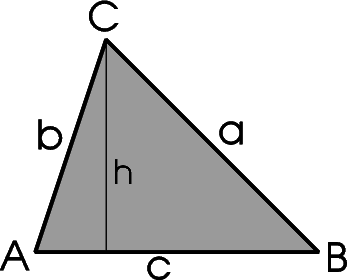
\includegraphics[scale=0.4]{images/01_precalculo/teorema_seno.png}
\caption{Triángulo}
\end{figure}

\begin{observation}
Si $u$ y $v$ no nulos son ortogonales, entonces el ángulo entre ellos es $\pi/2 = 90^{\circ}$
\end{observation}

\begin{definition}[Proyección] \index{Física!Vectores!Proyección}
Si $A$ y $B$ son vectores, la \textbf{proyección} de $A$ sobre $B \neq 0$ es el vector que representamos en la siguiente figura

y se calcula como

$$ proy_B(A) = \frac{A \cdot B}{||B||} \frac{B}{||B||}$$

\end{definition}

\begin{figure}[h]
\centering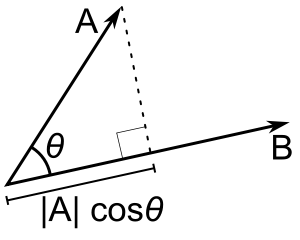
\includegraphics[scale=0.5]{images/01_precalculo/proyeccion_vector.png}
\caption{Proyección de un vector}
\end{figure}

\begin{proof}
Como $ A \cdot B = ||A|| \cdot ||B|| \cos(\theta)$, la norma de la proyección es $||A|| \cos(\theta) = \frac{A \cdot B}{||B||} $, y multiplicando por el versor asociado a $B$, es decir $\frac{B}{||B||}$, obtenemos el vector buscado $proy_B(A) = \frac{A \cdot B}{||B||} \frac{B}{||B||}$.
\end{proof}

\section{Sistema de fuerzas} \index{Física!Sistema de fuerzas}

En física, una \textbf{fuerza} es una acción capaz de imponer una aceleración sobre un cuerpo material.  Se representa mediante un vector. 

Recordemos las tres leyes del movimiento de \textbf{Newton}.

\begin{itemize}
\item La \textbf{primera ley de Newton} establece que todo cuerpo permanece en reposo o movimiento uniforme en linea recta, a menos que una fuerza actúe sobre él.

\item La \textbf{segunda ley de Newton} establece que la aceleración de un cuerpo de masa $m$ es igual a la fuerza resultante que actúa sobre el, dividido su masa, es decir

$$ a = \frac{F}{m} $$

dicho de otra forma

$$F = m \cdot a$$

Su unidad de medida es el Newton, $1 \ N = 1 \ \frac{kg \cdot m}{s^2} $

\item La \textbf{tercera ley de Newton} establece que si un cuerpo $A$ ejerce una fuerza $F_{A/B}$ sobre $B$, entonces $B$ ejerce una fuerza de igual magnitud y sentido contrario $F_{B/A}$ sobre $A$, es decir

$$ F_{A/B} = - F_{B/A} $$

\end{itemize}

Llamamos \textbf{sistema de fuerzas} al conjunto de fuerzas $F_1, F_2, \ldots, F_n$ que actúan sobre un cuerpo.

La \textbf{fuerza resultante} \index{Física!Sistema de fuerzas!Resultante} es $F_r = \sum_{i=1}^n F_i $, y la \textbf{fuerza equilibrante} \index{Física!Sistema de fuerzas!Equilibrante} es $F_e = - F_r$

En el plano, una fuerza $F = (x,y)N$ también la podemos representar como $F = (n,\alpha)$ donde $n = ||F||$ y $\alpha$ es el ángulo del vector $F$ con el eje $x$.

\section{Cinemática} \index{Física!Cinemática}

La \textbf{cinemática} es la parte de la física que estudia el \textbf{movimiento} de los cuerpos, abstrayendose de las causas que lo producen.  Los problemas que resuelve la cinemática son sobre calcular posición, velocidad y aceleración de un cuerpo.

El cuerpo vamos a modelarlo matemáticamente como un punto en el espacio, como si fuera un \textbf{partícula} puntual.

Para determinar su posición primero debemos fijar un \textbf{sistema de referencia}.  Es decir fijar un sistema de coordenadas ortogonales en el plano o el espacio.

De aquí en adelante sólo trabajaremos con partículas que se mueven sobre un plano que representaremos por $\mathbb{R}^2$.

La posición de una partícula queda entonces determinada por el \textbf{vector posición} $r$.

La \textbf{trayectoria} \index{Física!Cinemática!Trayectoria} que sigue una partícula es la función que determina el vector posición en función del tiempo, es decir determina la posición de la partícula en cada instante.

$$ \vec{x}(t) = (x_x(t), x_y(t))$$

En la siguiente figura representamos una trayectoria en el plano

\begin{figure}[h]
\centering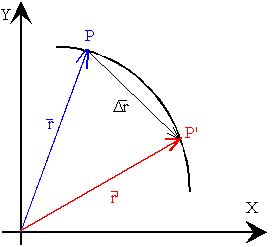
\includegraphics[scale=0.5]{images/01_precalculo/desplazamiento.png}
\caption{Desplazamiento}
\end{figure}

Supongamos que consideramos un intervalo de tiempo $\triangle t = t_f - t_i$.  La \textbf{posición inicial} es $ x_i = x(t_i)$ y la \textbf{posición final} es $x_f = x(t_f)$.  Entonces

\begin{itemize}
\item El \textbf{desplazamiento} es 

$$\triangle x = x(t_f) - x(t_i)$$  

\item La \textbf{distancia recorrida} es $||\triangle x||$

\item La \textbf{velocidad media} es $ v_m = \frac{\triangle x}{ \triangle t} = \frac{x(t_f) - x(t_i)}{\triangle t}$

\item La \textbf{velocidad instantánea} es 

$$ v(t) = \lim_{\triangle t \to 0} \frac{x(t + \triangle t) - x(t)}{\triangle t}$$

\item La \textbf{aceleración media} es $ a_m = \frac{\triangle v}{ \triangle t} = \frac{v(t_f) - v(t_i)}{\triangle t}$

\item La \textbf{aceleración instantánea} es 

$$ a(t) = \lim_{\triangle t \to 0} \frac{v(t+\triangle t) - v(t)}{\triangle t}$$

\end{itemize}

\subsection{Movimiento rectilíneo uniforme (MRU)}

La trayectoria se dice que está en \textbf{movimiento uniforme} también conocido como \textbf{movimiento rectilíneo uniforme} (MRU) \index{Física!Cinemática!MRU} cuando se puede expresar como

$$ x(t) = x_i + v (t - t_i) $$

donde $x_i \in \mathbb{R}^n$ es la posición inicial, es decir $x_i = x(t_i)$, y $v \in \mathbb{R}^n$ es la velocidad (constante).

En este caso, la partícula se mueve sobre una recta a velocidad constante.  La aceleración es nula en todo momento.

\subsection{Movimiento uniformemente variado (MPUV, MRUV)}

La trayectoria se dice que está en \textbf{movimiento uniformemente acelerado} también conocido como \textbf{movimiento uniformemente variado} (MUV) \index{Física!Cinemática!MUV} cuando se puede expresar como

$$ x(t) = x_i + v_i (t-t_i) + \frac{1}{2}a (t-t_i)^2 $$

Donde $x_i \in \mathbb{R}^n$ es la posición inicial, es decir $x_i = x(t_i)$, además $v_i \in \mathbb{R}^n$ es la velocidad inicial, es decir $v_i = v(t_i)$, y $a \in \mathbb{R}^n$ es la aceleración (constante).

La velocidad resulta entonces

$$ v(t) = v_i + a(t-t_i) $$

El MUV lo podemos clasificar según si es rectilíneo o no:

\begin{itemize}
\item Cuando la velocidad inicial $v_i$ es un vector paralelo a la aceleración $a$, la partícula se mueve sobre una recta, y se dice la trayectoria está en \textbf{movimiento rectilíneo uniformemente variado} (MRUV) \index{Física!Cinemática!MRUV}.  

Por ejemplo el tiro vertical (ver \ref{tiro_oblicuo}) es un MRUV.

\item En caso contrario, cuando el vector velocidad inicial $v_i$ no es paralelo al vector aceleración $a$, la partícula se mueve sobre una parábola, y se dice que la trayectoria está en \textbf{movimiento parabólico uniformemente variado} (MPUV) \index{Física!Cinemática!MPUV}.  

Por ejemplo el tiro oblicuo (ver \ref{tiro_oblicuo}) es un MPUV.
\end{itemize}

\subsection{Caída de cuerpos (Tiro oblicuo y vertical)}

La fuerza de gravedad atrae los cuerpos hacia la tierra con una aceleración con intensidad de 

$$ |g| = 9.8 \frac{m}{s^2}$$

Se denomina \textbf{proyectil} todo cuerpo que se mueve sólamente sujeto a una velocidad inicial, y a la fuerza que ejerce su propio peso por la acción de la gravedad, sin considerar otras fuerzas como la resistencia del aire.

Es decir que su trayectoria se puede expresar como

$$ x(t) = x_i + v_i (t-t_i) + \frac{1}{2} g (t-t_i)^2 $$

con $x_i = (x_i, y_i)$ la posición cuando $t= t_i$, $v_i = (v_x,v_y)$ la velocidad cuando $t=t_i$, y $g = (0, -9.8)$.

Si el ángulo entre $v_i$ y la horizontal es de $90^{\circ}$ decimos que es \textbf{tiro vertical} \label{tiro_vertical} \index{Física!Cinemática!Tiro vertical}.  Sinó decimos que es \textbf{tiro oblicuo} \label{tiro_oblicuo}. \index{Física!Cinemática!Tiro oblicuo}

\begin{example}
Si lanzamos un proyectil con $||v_i|| = 400 m/s$ y un ángulo de elevación de $30^{\circ}$.  Considerando $g = 10 m/s^2$.

Entonces la velocidad inicial es

\begin{eqnarray*}
v_i &=& 400 ( \cos(30^{\circ}), \sin(30^{\circ})) \\
 &=& 400 ( \frac{\sqrt{3}}{2}, \frac{1}{2}) \\
 &=& 200 ( \sqrt{3}, 1) \\
 &=& ( 200 \sqrt{3}, 200) 
\end{eqnarray*}

Digamos que la posición inicial es $x_i = (0,0)$.  Luego tenemos que la trayectoria es

$$ x(t) = (0,0) + ( 200 \sqrt{3}, 200) t + \frac{1}{2} (0, -10) t^2 $$

y su velocidad

$$ v(t) = (200\sqrt{3}, 200) + (0, -10) t $$

Luego, a los 5 segundos está en $x(5) = (1000 \sqrt{3}, 875)$

La velocidad a los 5 segundos es $v(5) = (200 \sqrt{3}, 150)$

Se encontrará a 1000 metros de altura cuando

$$ 200 t - 5 t^2 = 1000 $$

Es decir cuando $t_1 = 20 - 10\sqrt{2} \approx 5.85786 $ y tambien cuando $t_2 = 20 + 10\sqrt{2} \approx 34.1421$

La altura máxima alcanzada por el proyectil es cuando $v_y = 0$ es decir

$$ 200 - 10t = 0 $$

O sea cuando $t = 20$, y la altura alcanzada es $x_y(20) = 2000$, en ese instante tiene un velocidad de $v(20) = (200 \sqrt{3}, 0)$

El alcance máximo ocurre cuando $x_y(t) = 0$ es decir cuando

$$ 200 t - 5t^2 = 0 $$

O sea, cuando $t = 0$ está en el punto inicial, el otro es $t = 40$.  Dicho alcance es $x_x(40) = 8000 \sqrt{3}$.  La velocidad con la que llega es $v(40) = (200 \sqrt{3}, -200)$
\end{example}

%%%%%%%%%%%%%%%%%%%%%%%%%%%%%%%%%%%%%%%%%%%%%%%%%%%%%%%%%%%%%%%%%%%%%%%%%%%%%%%%
% Precálculo
%
% Copyright (c) 2016 Damián Silvestre. Permission is granted to copy, 
% distribute and/or modify this document under the terms of the 
% GNU Free Documentation License, Version 1.3 or any later version published by
% the Free Software Foundation; with no Invariant Sections, no 
% Front-Cover Texts, and no Back-Cover Texts. 
%
% Details of the GNU FDL can be found here: 
% http://www.gnu.org/licenses/licenses.html
%
%%%%%%%%%%%%%%%%%%%%%%%%%%%%%%%%%%%%%%%%%%%%%%%%%%%%%%%%%%%%%%%%%%%%%%%%%%%%%%%

\part{Precálculo}

\chapter{Nociones de lógica}

\section{Lógica proposicional}

\begin{definition}
Una \textbf{proposición} (P) \index{Lógica!Proposición} es un enunciado que tiene un valor de verdad, es decir que puede considerarse como \textbf{verdadero} (\textbf{V}) o \textbf{falso} (\textbf{F}).
\end{definition}

\begin{definition}
Se pueden crear nuevas proposiciones a partir de otras utilizando \textbf{conectivos lógicos}. \index{Lógica!Conectivos lógicos}

Definimos a continuación los principales conectivos lógicos a partir de sus \textbf{tablas de verdad}. \index{Lógica!Tabla de verdad}

\begin{itemize}
\item \textbf{Negación}: \index{Lógica!Conectivos lógicos!Negación}

\begin{tabular}{ |c|c| }
\hline
$P$ & $\neg P$  \\
\hline  
V & F  \\
F & V  \\
\hline
\end{tabular}

Ejemplo: \textbf{No} está lloviendo.

\item \textbf{Conjunción}: \index{Lógica!Conectivos lógicos!Conjunción}

\begin{tabular}{ |c|c|c| }
\hline
$P$ & $Q$ & $P \wedge Q$  \\
\hline  
V & V & V  \\
V & F & F  \\
F & V & F  \\
F & F & F  \\
\hline
\end{tabular}

Está lloviendo \textbf{y} está nublado.

\item \textbf{Disyunción}: \index{Lógica!Conectivos lógicos!Disyunción}

\begin{tabular}{ |c|c|c| }
\hline
$P$ & $Q$ & $P \vee Q$  \\
\hline  
V & V & V  \\
V & F & V  \\
F & V & V  \\
F & F & F  \\
\hline
\end{tabular}

Ejemplo: Está lloviendo \textbf{o} está soleado.

\item \textbf{Disyunción excluyente}: \index{Lógica!Conectivos lógicos!Disyunción excluyente}

\begin{tabular}{ |c|c|c| }
\hline
$P$ & $Q$ & $P \vee Q$  \\
\hline  
V & V & F  \\
V & F & V  \\
F & V & V  \\
F & F & F  \\
\hline
\end{tabular}

Ejemplo: \textbf{O bien} está soleado, \textbf{o bien} está nublado.

\item \textbf{Condicional}: \index{Lógica!Conectivos lógicos!Condicional}

\begin{tabular}{ |c|c|c| }
\hline
$P$ & $Q$ & $P \Rightarrow Q$  \\
\hline  
V & V & V  \\
V & F & F  \\
F & V & V  \\
F & F & V  \\
\hline
\end{tabular}

Ejemplo: Si está soleado, \textbf{entonces} es de día.

\item \textbf{Bicondicional}: \index{Lógica!Conectivos lógicos!Bicondicional}

\begin{tabular}{ |c|c|c| }
\hline
$P$ & $Q$ & $P \Leftrightarrow Q$  \\
\hline  
V & V & V  \\
V & F & F  \\
F & V & F  \\
F & F & V  \\
\hline
\end{tabular}

Ejemplo: Está nublado \textbf{si y sólo si} hay nubes visibles.

\end{itemize}

\end{definition}



\chapter{Números y geometría}

\section{Conjuntos}

\begin{definition}[Conjunto] \index{Conjunto}
Un \textbf{conjunto} \label{conjunto} es una colección de objetos, tal que si uno tiene un objeto cualquiera, puede determinar si está o no en la colección, o sea si \textbf{pertenece} o no.

Los objetos que pertenecen al conjunto se llaman los \textbf{elementos} del conjunto.

Si $A$ es un conjunto, y $x$ un elemento de $A$, lo denotamos $x \in A$.  Si $y$ no es un elemento de $A$, lo denotamos $y \not\in A$.

Si $A$ y $B$ son conjuntos, para todo $x \in A$ se tiene que $x \in B$, decimos que $A$ es un \textbf{subconjunto} de $B$  y lo denotamos $A \subseteq B$.  Si $A \subseteq B$ y $B \subseteq A$, los conjuntos $A$ y $B$ tienen los mismos elementos, y decimos que los conjuntos son \textbf{iguales}, es decir $A = B$.
\end{definition}

\begin{example}  
Algunos ejemplos de conjuntos son

\begin{enumerate} 
\item $ A = \{ \textrm{casa}, \textrm{arbol}, \textrm{vaca} \} $
\item $ B = \{ x \in \mathbb{R} : x \leq 23 \} $
\item $ C = \{ 2 , 4 , 77 \}$
\item $ D = \{-1, 1\} $
\end{enumerate}

El conjunto $A$ se describió por extensión, mientras que el conjunto $B$ por comprensión.

Si un elemento pertenece a un conjunto se lo denota con $\in$

Siguiendo con el ejemplo: $ \textrm{casa} \in A $, $ 11 \in B$.
\end{example}

\begin{definition}[Operaciones con conjuntos] \index{Conjunto!Operaciones}
Sean $A$ y $B$ conjuntos.  

La \textbf{unión} \index{Conjunto!Operaciones!Unión} de $A$ con $B$ es

$$A \cup B = \{ x / x \in A \vee x \in B \}$$

La \textbf{intersección} \index{Conjunto!Operaciones!Intersección} de $A$ con $B$ es

$$A \cap B = \{ x / x \in A \wedge x \in B \}$$

La \textbf{diferencia} \index{Conjunto!Operaciones!Diferencia} de $A$ con $B$ es

$$A - B = \{ x \in A / x \not\in B\}$$

Si fijamos un conjunto $U$ como conjunto universal, el \textbf{complemento} \index{Conjunto!Operaciones!Complemento} de cualquier subconjunto $A \subseteq U$ es $U-A$, y lo denotamos por $A^c$
\end{definition}

\begin{example}
Algunos ejemplos de operaciones entre conjuntos

\begin{itemize}
\item $ E = A \cup B$

\item $ F = B \cap C = \{2, 4\}$

\item $ B - C = \{ x \in \mathbb{R} : (x \leq 23) \wedge (x \neq 2) \wedge (x \neq 4) \} $

\item Considerando $ D \subseteq B$ tenemos $D^c = \{ x \in \mathbb{R} : x \leq 23 \wedge x \neq -1 \wedge x \neq 1\} = \{ x \in B : x \neq -1 \wedge x \neq 1 \}$

\end{itemize}
\end{example}

\begin{definition}[Producto Cartesiano] \index{Conjunto!Producto Cartesiano}
Si $A$ y $B$ son conjuntos, el producto cartesiano de $A$ con $B$ es el conjunto de todos los pares ordenados $(a,b)$ con $a \in A$ y $b \in B$, es decir

$$ A \times B = \{(a,b) : a \in A, b \in B \}$$

Dados $(a,b)$ y $(c,d)$ elementos de $A \times B$, se dice que $(a,b) = (c,d)$ si y sólo si $a = c$ y $b = d$.
\end{definition}

\begin{example}
Siguiendo con el ejemplo: 

\begin{eqnarray*}A \times D = \{(\textrm{casa},-1), (\textrm{arbol}, -1), (\textrm{vaca},-1), \\ 
(\textrm{casa},1), (\textrm{arbol},1), (\textrm{vaca},1)\} \end{eqnarray*}
\end{example}

\begin{definition}[Cardinal] \index{Conjunto!Cardinal}
Si un conjunto $A$ tiene una cantidad finita de elementos, decimos que es un \textbf{conjunto finito}, y llamamos \textbf{cardinal} a la cantidad de elementos que posee.

Lo denotamos por $|A|$ o por $\# A$.

Si no, decimos que $A$ tiene \textbf{cardinal infinito} $|A| = \infty$
\end{definition}

\begin{example}
Siguiendo con nuestros ejemplos

\begin{itemize}
\item $ |A| = 3$
\item $ |C \cup D| = 5$
\item $ |B| = \infty $
\item $ \# \mathbb{R} = \infty$
\end{itemize}
\end{example}

\subsection{Relaciones y Funciones}

\begin{definition}[Relación] \index{Conjunto!Relación}
Dados $A$ y $B$ conjuntos, una \textbf{relación} \label{relacion} de $A$ en $B$ es un subconjunto de $A \times B$.

Sea $R$ una relación.  Si $(a,b) \in R$, también lo denotamos $a R b$.
\end{definition}

\begin{example}
Por ejemplo, una relación de $A$ en $D$ podría ser:

$$ R = \{(\textrm{casa},-1), (\textrm{arbol},-1), (\textrm{casa},1) \} $$
\end{example}

\begin{definition}
Sea $R$ una relación de $A$ en $A$.  Se dice que es

\begin{itemize}

\item reflexiva: si $xRx$ para todo $x \in A$.

\item simétrica: si $xRy$ implica que $yRx$ para todos $x,y \in A$.

\item antisimétrica: si $xRy$ y $yRx$ implica que $y=x$.

\item transitiva: si $xRy$ y $yRz$ implica que $xRz$.
\end{itemize}
\end{definition}

\begin{definition}
Una relación $R$ de $A$ en sí mismo que es \emph{reflexiva}, \emph{simétrica} y \emph{transitiva}, se dice que es una \textbf{relación de equivalencia}, y se suele denotar $\equiv$.  

Si $R$ es una relación de equivalencia en $A$, dado $x \in A$, el conjunto de los los $y \in A$ tales que $x R y$ se llama la \textbf{clase de equivalencia de $x$}, y se denota

$$[x] = \{y \in A : yRx \}$$
\end{definition}

\begin{example}
Por ejemplo, en $\mathbb{Z}$, la relación $xRy$ sii $3 | y-x$ es una relación de equivalencia.  Bajo esta relación de equivalencia se tiene que $5 \equiv 11$, pues $3 | (11-5) = 6$.  Esta relación de equivalencia tiene tres clases de equivalencias 

\begin{eqnarray*}\overline{0} &=& \{0 + 3k : k \in \mathbb{Z} \} \\
\overline{1} &=& \{1 + 3k : k \in \mathbb{Z} \} \\
\overline{2} &=& \{2 + 3k : k \in \mathbb{Z} \} \end{eqnarray*}

Uniendo todas las clases de equivalencias, obtenemos el conjunto completo

$$ \mathbb{Z} = \overline{0} \cup \overline{1} \cup \overline{2}$$
\end{example}


\begin{definition}
Una relación $R$ de $A$ en sí mismo que es \emph{reflexiva}, \emph{antisimétrica} y \emph{transitiva}, se dice que es una \textbf{relación de orden} \label{orden} (parcial), y se suele denotar $\leq$.

Un conjunto con un orden parcial se dice que es un \textbf{conjunto ordenado}.
\end{definition}

\begin{example}
Por ejemplo en $\mathbb{Z}$ la relación $xRy$ sii $x | y$ ($x$ divide a $y$) es una relación de orden.
\end{example}

\begin{definition}
Si $\leq$ es una relación de orden en $A$, y si $x,y \in A$, entonces decimos que $x$ e $y$ son \textbf{comparables} si se cumple que $x \leq y$ o bien que $y \leq x$.  En caso contrario decimos que $x$ e $y$ son \textbf{no comparables}.
\end{definition}

\begin{example}
Por ejemplo, si en $\mathbb{Z}$ tomamos la relación $x \leq y$ sii $ x | y$, entonces $3$ y $5$ son elementos no comparables, pues $3 \not| 5$ y $5 \not| 3$.
\end{example}

\begin{definition} \label{orden_total}
Una relación de orden en la que $x \leq y$ o $y \leq x$ para todo $x,y \in A$ se dice que es una relación de \textbf{orden total}.

Es decir que un orden total es una relación de orden en la que todo par de elementos es comparable.

Un conjunto con un orden total se dice que es un \textbf{conjunto totalmente ordenado}
\end{definition}

\begin{example}
Por ejemplo, en $\mathbb{R}$ la relación $xRy$ sii $x \leq y$ es una relación de orden total.
\end{example}


\begin{definition}[Máximo, mínimo, cotas, supremo, etc] \label{maximo}

Sea $A$ un conjunto ordenado.  

\begin{itemize}

\item Si existe $z \in A$ tal que para todo $x \in A$ se tiene que $x \leq z$ se dice que $z$ es el \textbf{máximo} \index{Orden!máximo} de $A$.

\item Si existe $z \in A$ tal que para todo $x \in A$ se tiene que $x \geq z$ se dice que $z$ es el \textbf{mínimo} \index{Orden!mínimo} de $A$.

\item Si para $z \in A$ se cumple que para todo $x \geq z$ se tiene que $x = z$ se dice que $z$ es un \textbf{elemento maximal} \index{Orden!maximal} de $A$.

\item Si para $z \in A$ se cumple que para todo $x \leq z$ se tiene que $x = z$ se dice que $z$ es un \textbf{elemento minimal} \index{Orden!minimal} de $A$.

\end{itemize}

Sea $B \subseteq A$, entonces

\begin{itemize}

\item Si existe $z \in A$ tal que para todo $b \in B$ se tiene que $b \leq z$, decimos que $z$ es una \textbf{cota superior} \index{Orden!cota superior} de $B$.

\item Si existe $z \in A$ tal que para todo $b \in B$ se tiene que $b \geq z$, decimos que $z$ es una \textbf{cota inferior} \index{Orden!cota inferior} de $B$.

\item Si el conjunto de cotas superiores de $A$ tiene un mínimo $z$, decimos que $z$ es el \textbf{supremo} \index{Orden!supremo} de $A$.

\item Si el conjunto de cotas inferiores de $A$ tiene un máximo $z$, decimos que $z$ es el \textbf{ínfimo} \index{Orden!ínfimo} de $A$.

\end{itemize}

\end{definition}

\begin{definition}[Función] \index{Función} \label{funcion}

Una \textbf{función} de $A$ en $B$ es una relación tal que para todo $a \in A$ existe $b \in B$ de forma tal que $(a,b) \in R$, y además dicho $b$ es único, es decir que si se tiene $(a,b) \in R$ y $(a,c) \in R$, entonces $b=c$.

Se la denota de la forma $f : A \to B$, y si se tiene $(a,b) \in f$, también se escribe $f(a) = b$, y se dice que la imagen de $a$ por $f$ es $b$.

\begin{itemize}
\item El conjunto $A$ se llama \textbf{dominio} \index{Función!Dominio} y el conjunto $B$ se llama \textbf{codominio} \index{Función!Codominio} de la función.

\item Dado $C \subseteq A$, el conjunto $f(C) = \{b \in B : \exists c \in C, f(c) = b\}$ se llama imagen de $C$ por $f$.  El conjunto $f(A)$ se llama la \textbf{imagen} \index{Función!Imagen} de $f$, y se denota $Im(f)$.  Es decir

$$ Im(f) = \{ b \in B : \exists a \in A, f(a) = b \} $$

\item La \textbf{gráfica} de la función es la relación funcional que las define, es decir

$$ Graf(f) = \{ (x,y) \in A \times B : y = f(x) \} $$

\item Si $Y \subseteq B$ llamamos \textbf{preimagen} de $Y$ por $f$ al conjunto

$$ f^{-1}(Y) = \{a \in A : f(a) \in Y \}$$
\end{itemize}
\end{definition}

\begin{observation}
Observamos que en ningún momento en la definición de función se requiere tener una expresión tipo \emph{fórmula} para calcular los elementos de la imagen.
\end{observation}

\begin{example}

Siguiendo con los mismos conjuntos de los ejemplos anteriores, podemos definir una función

\begin{eqnarray*} f : A &\to& B \\
f(\textrm{casa}) &=& -1 \\
f(\textrm{arbol}) &=& 21 \\
f(\textrm{arbol}) &=& 21 \\
f(\textrm{vaca}) &=& 12 \end{eqnarray*} 

\end{example}

\section{Conjuntos numéricos}

\begin{definition}[Números reales] \index{Conjunto!Números reales}
El principal conjunto con el que vamos a trabajar es el conjunto de los \textbf{números reales}, que denotaremos $\mathbb{R}$.  En este conjunto están definidas las operaciones suma $+$ y producto $\cdot$ con las siguientes propiedades:

Para todo $x,y,z \in \mathbb{R}$

\begin{itemize}

\item Asociativa para la suma

$x+(y+z) = (x+y)+z$

\item Neutro para la suma: existe $0 \in \mathbb{R}$

$x+0 = 0+x = x$

\item Inverso para la suma: para todo $x$ existe $-x \in \mathbb{R}$ tal que

$x + (-x) = (-x) + x = 0$

\item Conmutatividad de la suma

$x+y = y+x$

\item Asociatividad del producto

$x(yz) = (xy)z$

\item Neutro del producto: existe $1 \in \mathbb{R}$ tal que

$1 \cdot x = x \cdot 1 = x$

\item Inverso del producto: para todo $x \neq 0$ existe $x^{-1}$ tal que

$x \cdot x^{-1} = x^{-1} \cdot x = 1$

\item Conmutatividad del producto

$xy = yx$

\item Distributiva

$x(y+z) = xy + xz$

$(x+y)z = xz + yz$

\item Se tiene un orden total $\leq$ tal que si $x \leq y$ y $z \in \mathbb{R}$ entonces

$x+z \leq y+z$

y además si $z \geq 0$ entonces

$xz \leq yz$ 

\item Todo subconjunto $A \subseteq \mathbb{R}$ acotado superiormente tiene un supremo.

\end{itemize}
\end{definition}

\begin{definition}[Números naturales] \index{Conjunto!Números naturales}
Sea $A \subseteq \mathbb{N}$.  Decimos que $A$ es un \textbf{conjunto inductivo} si cumple las siguientes

\begin{itemize}

\item $1 \in \mathbb{N}$

\item Si $n \in \mathbb{N}$ entonces $n+1 \in \mathbb{N}$

\end{itemize}

Definimos el conjunto de los \textbf{números naturales} $\mathbb{N}$ como la intersección de todos los conjuntos inductivos.  Es decir sus elementos son 

$$ \mathbb{N} = \{1,2,3,4,5, \ldots \} $$
\end{definition}

\begin{definition}[Números enteros] \index{Conjunto!Números enteros}
El conjunto de los \textbf{números enteros} contiene a los naturales, y le agrega el $0$ y los inversos aditivos, es decir

$$ \mathbb{Z} = \{\ldots, -4,-3,-2,-1,0,1,2,3, \ldots \}$$
\end{definition}

\begin{definition}[Números racionales] \index{Conjunto!Números racionales}
El conjunto de los \textbf{números racionales} satisface todas las propiedades de los reales salvo la del axioma del supremo.  Son los que podemos escribir como fracciones

$$ \mathbb{Q} = \{ \frac{p}{q} : p,q \in \mathbb{Z}, q \neq 0 \} $$

y se tiene que $\frac{a}{b} = \frac{c}{d}$ si y sólo si $ad = cb$.
	
Entre dos racionales siempre existe otro, por ejemplo sean $x,y \in \mathbb{Q}$ con $x < y$.  Entonces $z = \frac{x+y}{2}$ es tal que $x < z < y$.  Lo mismo puede decirse entre dos reales $x<y$ en general.
\end{definition}

\begin{definition}[Números complejos] \index{Conjunto!Números complejos}
El conjunto de los \textbf{números complejos} consisten en agregarle a los reales un nuevo número $i \in \mathbb{C}$ tal que $i^2 = -1$

$$ \mathbb{C} = \{ a + b i : a,b \in \mathbb{R}, i^2 = -1 \}$$

Si identificamos $a+bi$ con el par ordenado $(a,b)$ podemos identificar $\mathbb{C}$ con $\mathbb{R}^2$ con la siguiente regla de multiplicación

$$ (a+bi)(c+di) = (ac - bd) + (ad + bc) i$$

o sea

$$ (a,b)(c,d) = (ac - bd, ad + bc)$$
\end{definition}



\section{Divisibilidad en $\mathbb{Z}$}

\begin{definition}[Divisibilidad] \index{Conjunto!Números enteros!Divisibilidad}
Sean $a,b,c \in \mathbb{Z}$ tales que $a = bc$.  Decimos entonces que $b$ \textbf{divide} a $a$ y lo denotamos $b | a$.  También decimos que $b$ es un \textbf{divisor} de $a$, o que $a$ es divisible por $b$.  El conjunto de divisores de $a$ lo denotamos $Div(a)$

Si $b$ no divide a $a$, es decir no existe $c$ tal que $bc = a$, lo denotamos $b \not| a$.

Si $2|x$ decimos que $x$ es \textbf{par}, de lo contrario $2 \not| x$ y decimos que $x$ es \textbf{impar}.
\end{definition}

\begin{definition}[Número primo] \index{Conjunto!Números enteros!Número primo}
Todo $x \in \mathbb{Z}$ es divisible por $1,-1,x,-x$.  Si $x \neq 0,1,-1$ y sus únicos divisores son $1,-1,x,-x$, decimos que $x$ es un \textbf{número primo}.
\end{definition}

\begin{definition}[MCD, MCM, coprimos] \index{Conjunto!Números enteros!MCD,MCM,coprimos}
Sean $x,y \in \mathbb{Z}$.  El \textbf{máximo común divisor} (MCD) entre $x$ e $y$ es el máximo de los divisores comunes, y lo denotamos $(x:y)$

El \textbf{mínimo común múltiplo} (MCM) entre $x$ e $y$ es el mínimo de los múltiplos comunes, y lo denotamos $[x:y]$

Se verifica la siguiente propiedad: $[x:y] (x:y) = x \cdot y$

Decimos que $x$ e $y$ son \textbf{coprimos} si y sólo si $(a:b) = 1$
\end{definition}

\begin{theorem}[Teorema fundamental de la aritmética (TFA)] \index{Conjunto!Números enteros!TFA}
Para todo $x \in \mathbb{Z}$, tal que $x \neq 0, 1, -1$, existen números primos distintos $p_1, p_2, \ldots, p_n \in \mathbb{Z}$ positivos, y números naturales $a_1, a_2, \ldots, a_n \in \mathbb{N}$ de forma tal que

$$ x = \pm p_1^{a_1} p_2^{a_2} \ldots p_n^{a_n} $$

donde $\pm$ es el signo de $x$, y además dicha escritura es única salvo el orden de los factores.
\end{theorem}

\begin{observation}[MCD y MCM usando TFA]
Una regla para determinar $(x:y)$ consiste en descomponer $x$ e $y$ en sus factores primos, y luego multiplicar los factores comunes con su menor exponente.  Por ejemplo para calcular $(12,28)$ primero descompongo $12 = 2^3 \cdot 3$ y $28 = 2^2 \cdot 7$, entonces $(12:28) = 2^2 = 4$.
	
Y para determinar $[x:y]$ multiplicamos los factores comunes con su mayor exponente.  Por ejemplo $[12:28] = 2^3 \cdot 3 \cdot 7 = 168$.	
\end{observation}

\section{Expresión decimal de un racional} \index{Conjunto!Números racionales!Expresión decimal}

Sea $\frac{a}{b} \in \mathbb{Q}$, entonces al efectuar la división podemos expresarlo en forma decimal, con una cantidad finita de decimales, o infinita periódica.

Ejemplos:

$\frac{1}{2} = 0.5$

$\frac{3}{2} = 1.5$

$\frac{1}{3} = 0.333333\ldots = 0.\overline{3}$

$\frac{3549}{990} = 3.5\overline{84}$

En este último ejemplo, para pasar de la notación decimal a la fraccionaria, realizamos la siguiente operación

$ \frac{3584 - 35}{990} = \frac{3549}{990} = \frac{1183}{330}$

\section{Intervalos}

\begin{definition}[Intervalo] \index{Conjunto!Números reales!Intervalo}

Un intervalo es un subconjunto $I \subseteq \RR$ tal que para todos $x,y \in I$ y todo $x < c < y$ se tiene que $c \in I$.

Los intervalos los podemos clasificar de la siguiente manera.  Sean $a,b \in \RR$ con $a<b$ entonces tenemos

\begin{itemize}

\item El intervalo finito abierto 

$(a,b) = \{ x \in \mathbb{R} : a < x < b \}$

\item El intervalo finito cerrado

$[a,b] = \{ x \in \mathbb{R} : a \leq x \leq b \}$

\item Los intervalos finitos semiabiertos

$(a,b] = \{ x \in \mathbb{R} : a < x \leq b \}$

$[a,b) = \{ x \in \mathbb{R} : a \leq x < b \}$

\item Los intervalos infinitos abiertos

$(a, +\infty) = \{ x \in \mathbb{R} : x > a \}$

$(-\infty, a) = \{ x \in \mathbb{R} : x < a \}$

\item Los intervalos infinitos cerrados

$[a, +\infty) = \{ x \in \mathbb{R} : x \geq a \}$

$(-\infty, a] = \{ x \in \mathbb{R} : x \leq a \}$

\end{itemize}
\end{definition}



\section{Valor absoluto}

\begin{definition}[Módulo o valor absoluto] \label{funcion_modulo} \index{Función!Ejemplos!Función módulo}
El \textbf{valor absoluto} (o módulo) es la siguiente función $| \cdot | : \mathbb{R} \to \mathbb{R}$

$$ |x| = \begin{cases} x & \textrm{ si } x \geq 0 \\ -x & \textrm{ si } x < 0 \end{cases} $$

\end{definition}

\begin{property}[del valor absoluto]
Se verifican: 

\begin{itemize}
\item $ |x| \geq 0 $ para todo $x \in \mathbb{R}$
\item Si $ |x| = 0$ entonces $x = 0$
\item $ |ab| = |a| |b|$
\item $|a+b| \leq |a| + |b|$

\item $|a| < b$ si y sólo si $-b < a < b$

\item $|a| > b$ si y sólo si $a > b$ o bien $a < -b$

\item $|a| = b$ si y sólo si $a=b$ o bien $a = -b$

\end{itemize}
\end{property}

\begin{definition}[Distancia] \index{Conjunto!Números reales!distancia}
Sean $x, y \in \mathbb{R}$, definimos la \textbf{distancia} entre $x$ e $y$ como 

$$d(x,y) = |y - x|$$

\end{definition}

\begin{property}[de la distancia] Se verifican para todo $x,y,z \in \mathbb{R}$

\begin{itemize}
\item $d(x,y) \geq 0$
\item $d(x,y) = 0$ si y sólo si $x=y$
\item $d(x,y) = d(y,x)$
\item $d(x,z) \leq d(x,y) + d(y,z)$
\end{itemize}

\end{property}


\section{Sobre exponentes y raíces}

\begin{definition}[Potencia $n$-ésima] \index{Conjunto!Números reales!Potencia y raíz}
Si $x \in \mathbb{R}$ y $n \in \mathbb{N}$ definimos $x$ a la $n$-ésima \textbf{potencia} como

$$x^n = \underbrace{x \cdot x \cdot \ldots \cdot x}_{n \ veces} = y$$

A $x$ lo llamamos \textbf{base}, a $n$ lo llamamos el \textbf{exponente}, y a $y$ potencia.
\end{definition}

\begin{observation}
Si $n$ es par, $y \geq 0$.  Si $n$ es impar, el signo de $x$ y de $y$ coinciden.
\end{observation}	

\begin{definition}[Raíz $n$-ésima]
Ahora al revés, supongamos que conocemos $y \in \mathbb{R}$, y $n \in \mathbb{N}$, llamamos \textbf{raíz $n$-ésima} de $x$, y lo denotamos $\sqrt[n]{x} = y$, al número $y$ tal que $y^n = x$.
\end{definition}	

\begin{observation}
Por la observación anterior, si $x < 0$ y \textbf{$n$ es par}, no queda definida en $\mathbb{R}$ dicha raíz.  Por ejemplo $\sqrt{-1} \not\in \mathbb{R}$.  Resulta que en los otros casos la raíz existe y es única (en $\mathbb{R}$).
\end{observation}

\begin{property}
Si $x,y \in \mathbb{R}$ y $n$ es impar

$$ (xy)^n = x^n y^n $$

Si $x,y \geq 0$ y $n$ es par también se cumple dicha igualdad.
\end{property}

\begin{definition}[Potenciación con números racionales y reales]
Extendemos la definición de potencia primero a los racionales mediante

\begin{itemize}
\item $x^{1/n} = \sqrt[n]{x}$ 
\item $x^{-n} = \frac{1}{x^n}$
\item $x^{p/q} = \sqrt[q]{x^p}$
\end{itemize}
	
La última definición nos permite potenciar con exponentes racionales.  

Si $x,n \in \mathbb{R}$, $x,n>0$, es posible definir $x^n$.  Por ahora este caso lo trabajamos sólamente con la calculadora.
	
\end{definition}


\section{Teorema de Pitágoras}

\begin{theorem}[Pitágoras] \index{Geometría!Teorema de Pitágoras}
Sea un triángulo rectángulo como el de la figura en color amarillo.

Llamamos $a$ y $b$ a sus catetos, y $c$ a su hipotenusa.  Entonces 

$$ c^2 = a^2 + b^2 $$
\end{theorem}

\begin{figure}[h]
\centering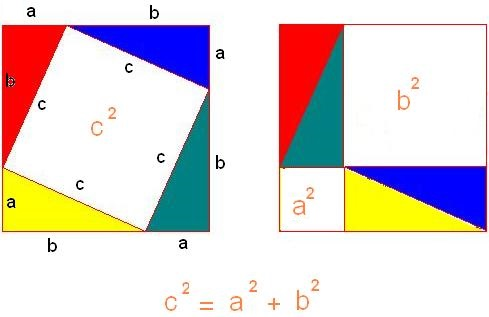
\includegraphics[scale=1]{images/01_precalculo/Pythagore.jpg}
\caption{Pitagoras}
\end{figure}

\begin{proof}
El área del cuadrado grande es 

$A = (a+b)(a+b) = a^2 + 2ab + b^2$

El área del cuadrado chico es $c^2$.  Pero además el área del cuadrado grande es igual a la del cuadrado chico mas cuatro veces el área del triángulo amarillo.  Es decir

$ a^2 + 2ab + b^2 = c^2 + 4 \frac{ab}{2} $

$ a^2 + 2ab + b^2 = c^2 + 2 ab $

$ a^2 + b^2 = c^2 $

como queríamos demostrar.
\end{proof}



\section{Números irracionales} \index{Conjunto!Números reales!Irracionales}

Veamos que algunos números reales no son racionales.  A los números reales que no son racionales los llamamos \textbf{irracionales}.

Supongamos que tenemos un cuadrado de lado 1 como en la figura.

\begin{figure}[h]
\centering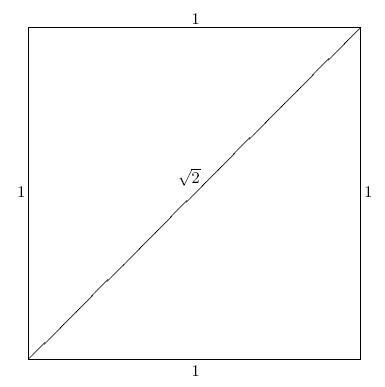
\includegraphics[scale=0.5]{images/01_precalculo/unit-square-with-diagonal.jpg}
\caption{Diagonal de un cuadrado}
\end{figure}

Queremos determinar el largo $c$ de su diagonal.  Por el teorema de pitágoras sabemos que $c^2 = 1^2 + 1^2 = 2$, es decir que $c = \sqrt{2}$.  

\begin{theorem}
$\sqrt{2} \not\in \QQ$
\end{theorem}

\begin{proof}
Supongamos que $\sqrt{2}$ es un número racional, es decir $\sqrt{2} = p/q$, con $p,q \in \mathbb{N}$ y coprimos, es decir $(p:q) = 1$, de forma que la fracción esté expresada en forma irreducible.

Elevando al cuadrado se tiene

$ \frac{p^2}{q^2} = 2$

$ p^2 = 2 q^2$

O sea que $p^2$ es par.  Por el teorema fundamental de la aritmética esto implica que $p$ es par.  O sea que $p = 2m$.  Luego

$ 4m^2 = 2q^2$

$ 2m^2 = q^2$

Con un razonamiento análogo al anterior vemos que $q$ es par.  Esto es absurdo pues $p$ y $q$ eran coprimos.  El absurdo provino de suponer que $\sqrt{2}$ es racional.  Por lo tanto $\sqrt{2}$ no es racional.
\end{proof}

\begin{problem}
Prueba gráfica de que $32.5 = 31.5$.  ¿Cómo es posible?
\end{problem}

\begin{figure}[h]
\centering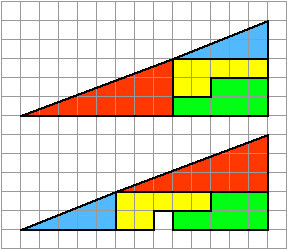
\includegraphics[scale=0.6]{images/01_precalculo/ilusion_triangulo.jpg}
\caption{Ilusión triángulo}
\end{figure}

Rta: Es una ilusión óptica.  El de arriba pareciera ser un triángulo de area $ \frac{13 \cdot 5}{2} = 32.5$.  Y el de abajo es reacomodar las fichas pero parece un triángulo con un cuadrado menos, es decir una region con área $31.5$.  

Pero en realidad ninguna de las dos figuras es un triángulo.  Basta ver que los ángulos de los triángulos rojo y azul no son iguales, sus tangentes (opuestos/adyancete) son $3/8 = 0.375 \neq 0.4 = 2/5 $.



\chapter{Polinomios}

\begin{definition}[Monomio] \index{Polinomio!Monomio}
Un \textbf{monomio} es una expresión en la que intervienen números reales, y variables, sólamente relacionadas por multiplicación (y potenciación con exponente natural).  

El \textbf{grado} del monomio es la suma de los exponentes de las variables.
\end{definition}

\begin{example}
Algunos monomios y sus grados:

\begin{itemize}
\item $12x^2y$ es de grado 3
\item $\pi z x^3$ es de grado 4
\item $-25 u^2$ es de grado 2
\end{itemize}
\end{example}

\begin{definition}[Polinomio] \index{Polinomio}
Un \textbf{polinomio} es una suma de monomios, y su \textbf{grado} es el grado del monomio de mayor \textbf{grado} que interviene en la suma.
\end{definition}

\begin{example}

Algunos polinomios y sus grados

\begin{itemize}
\item $12x^2y + \pi z x^3 $ es de grado 4
\item $3xy + z^2 - 3uv + x^3$ es de grado 3
\end{itemize}
	
\end{example}



\section{Polinomios en una indeterminada}

\begin{definition}[Polinomio en una variable] \index{Polinomio!Real}
En esta parte, sólamente vamos a trabajar con polinomios en una sóla variable ó indeterminada.  Al conjunto de todos los polinomios (con coeficientes en $\RR$) \textbf{en una sola variable} $x$ lo denotamos $\RR[x]$

Siempre podemos expresar un polinomio $p \in \RR[x]$ en la forma $p = \sum_{i=0}^n a_i x_i$, es decir

$$ p = a_0 + a_1 x + a_2 x^2 + \ldots + a_n x^n $$

con $a_n \neq 0$, y el grado del polinomio lo denotamos $gr(p) = n$

El polinomio nulo $p=0$ es el único polinomio que no tiene grado.

Decimos que el polinomio $p$ es \textbf{mónico} si $a_n = 1$.

Dos polinomios $p$  y $q$ son \textbf{iguales} si y sólo si sus coeficientes son iguales.  Es decir si $p = \sum_{i=0}^n a_i x^i$ y $q = \sum_{j=0}^m b_j x^j$ entonces $p=q$ si y sólo si $n=m$ y $a_i = b_i$ para todo $0 \leq i \leq n$
\end{definition}

\begin{example}
Algunos polinomios de $\RR[x]$
\begin{itemize}

\item $3x^2 + 2x -3$ es de grado 3
\item $\pi x + 8x^5 $ es de grado 5
\end{itemize}

\end{example}

\subsection{Operaciones con polinomios}

\begin{definition}[Suma y producto de polinomios] \index{Polinomio!Real!Suma y producto}
	
Sean $p = \sum_{i=0}^n a_i x^i$ y $q = \sum_{j=0}^m b_j x^j$.

Sea $r = max\{ n,m \}$

Entonces la \textbf{suma} la definimos como

$$ p+q = \sum_{k=0}^r (a_k+b_k) x^k $$

es decir se suma coeficiente a coeficiente.

El \textbf{producto} lo definimos como

$$ p \cdot q = \sum_{k=0}^{n+m} c_k x^k $$

donde 

$$ c_k = \sum_{i+j=k} a_i b_j $$

\end{definition}

\begin{observation}
Si $gr(p) = n$ y $gr(q) = m$ entonces $gr(pq) = n+m$
\end{observation}


\begin{definition}[Divisibilidad] \index{Polinomio!Real!Divisibilidad}
Si $p,q,r \in \mathbb{R}[x]$ y $p = qr$, decimos que $q$ \textbf{divide} a $p$, y lo denotamos $q|p$.
\end{definition}

\subsection{Algoritmo de división}

\begin{theorem}[Algoritmo de la división] \index{Polinomio!Real!Algoritmo de la división}
Si $p,q \in \mathbb{R}[x]$ entonces existen únicos polinomios $c,r$ tales que

$$ p = q \cdot c + r$$

con $r=0$ o $gr(r) < gr(q)$

Decimos que $p$ es el \textbf{dividendo}, $q$ el \textbf{divisor}, $c$ el \textbf{cociente}, y $r$ el \textbf{resto}.
\end{theorem}

\begin{definition}[Especialización] \index{Polinomio!Real!Especialización}
Sea $p \in \mathbb{R}[x]$, de forma $p = \sum_{i=0}^n$, y sea $\alpha \in \mathbb{R}$.  La \textbf{especialización} de $p$ en $\alpha$ es el número real

$$ p(\alpha) = \sum_{i=0}^n a_i \alpha^i $$
\end{definition}

\begin{definition}[Raíces y multiplicidad] \index{Polinomio!Real!Raíz y multiplicidad}

Si $p(\alpha) = 0$ se dice que $\alpha$ es una \textbf{raíz} (o un cero) de $p$.  

Decir que $\alpha \in \mathbb{R}$ es raíz de $p$ equivale a decir que $(x-\alpha)$ divide a $p$

Sea $\alpha \in \mathbb{R}$ raíz de $p \in \mathbb{R}[x]$, y sea $a \in \mathbb{N}$ tal que $(x-\alpha)^a | p$ pero $(x-\alpha)^{a+1} \not| p$.  Decimos que $a$ es la \textbf{multiplicidad} de $\alpha$ como raíz de $p$.

Si $a = 1$ se dice que $\alpha$ es \textbf{raíz simple} de $p$, sinó, $a>1$ y se dice que $\alpha$ es \textbf{raíz múltiple} de $p$.
\end{definition}


\begin{theorem}[del resto] \index{Polinomio!Real!Teorema del resto}
Sean $p, q \in \mathbb{R}[x]$, con $q = x - \alpha$.  El resto de dividir $p$ por $q$ es igual a $p(\alpha)$
\end{theorem}

\begin{proof}
Por el algoritmo de la división existen $c$ y $r$ tales que $p(x) = (x-\alpha) c(x) + r(x)$ con $gr(r) < gr(q) = 1$ o $r=0$.  Es decir $r$ constante.

Especializando en $\alpha$ obtenemos $p(\alpha) = r$.
\end{proof}

\begin{definition}[Polinomio irreducible] \index{Polinomio!Real!Irreducible}
Sea $p \in \mathbb{R}[x]$.  Decimos que $p$ es un polinomio \textbf{irreducible} si sus únicos divisores son los polinomios constantes y los polinomios de la forma $c \cdot p$ con $c$ constante.
\end{definition}

\begin{theorem}[Teorema Fundamental de la Aritmética para polinomios] \index{Polinomio!Real!TFA para polinomios}

Sea $p \in \mathbb{R}[x]$.  Entonces existen únicos $c \in \mathbb{R}$, polinomios irreducibles distintos $p_1, p_2, \ldots, p_n \in \mathbb{R}[x]$, y $a_1, a_2, \ldots, a_n \in \mathbb{N}$ de forma que

$$ p = c p_1^{a_1} p_2^{a_2} \ldots p_n^{a_n} $$

\end{theorem}

\begin{theorem}[Gauss] \index{Polinomio!Real!Teorema de Gauss}
Sea $P \in \mathbb{Z}[x]$, $p = a_0 + a_1x + a_2x^2 + \ldots + a_nx^n$, con $a_i \in \mathbb{Z}$ para $0 \leq i \leq n$, y $a_n \neq 0$.  Si $\alpha = \frac{p}{q} \in \mathbb{Q}$ es raíz de $P$, con $(p:q) = 1$, entonces $q | a_n$ y $p | a_0$.
\end{theorem}

\begin{proof}
Como $\alpha = p/q$ es raíz, se tiene que $P(p/q) = 0$, o sea

$a_0 + a_1 \frac{p}{q} + a_2 \frac{p^2}{q^2} + \ldots + a_{n-1} \frac{p^{n-1}}{q^{n-1}} + a_n \frac{p^n}{q^n} = 0$

multiplico por $q^n$

$a_0 q^n + a_1 p q^{n-1} + a_2 p^2 q^{n-2} + \ldots + a_{n-1} p^{n-1} q +  a_n p^n = 0$

saco factor común $p$

$a_0 q^n + p [a_1 q^{n-1} + a_2 p^1 q^{n-2} + \ldots + a_n p^{n-1}] = 0$

Como $p$ divide a $0$ y al segundo sumando, también divide a $a_0 q^n$, pero como $(p:q) = 1$ se tiene que $p | a_0$

Similarmente, sacando factor $q$

$q[a_0 q^{n-1} + a_1 p q^{n-2} + a_2 p^2 q^{n-3} + \ldots a_{n-1} p^{n-1}] + a_n p^n = 0$

Como $q$ divide a $0$ y al primer sumando, se tiene que $q$ divide a $a_n p^n$.  Pero como $(p:q) = 1$, se tiene que $q | a_n$.
\end{proof}

\begin{proposition}[Ecuación de primer grado] \index{Polinomio!Real!Ecuación lineal}
Una ecuación de \textbf{primer grado} (o \textbf{ecuación lineal}) es de la forma

$$ ax + b = 0 $$

con $a \neq 0$, y su única solución es $x = -b/a$.
\end{proposition}

\begin{proposition}[Ecuación de segundo grado] \index{Polinomio!Real!Ecuación cuadrática}
Una ecuación de \textbf{segundo grado} (o \textbf{ecuación cuadrática}) es de la forma

$$ ax^2 + bx + c = 0 $$

con $a \neq 0$.  Sus soluciones (en $\CC$) son dadas por la \textbf{fórmula resolvente}: \label{formula_resolvente}

$$ x_{1,2} = \frac{-b \pm \sqrt{b^2 - 4ac}}{2a}  $$

\end{proposition}

\begin{proof}
	
Divido por $a$

$ x^2 + \frac{b}{a}x + \frac{c}{a} = 0 $

completo cuadrado, es decir busco $\alpha, \beta \in \mathbb{R}$ tal que $(x-\alpha)^2 + \beta = x^2 + \frac{b}{a}x$, es decir

$ x^2 - 2\alpha x + \alpha^2 + \beta = x^2 + \frac{b}{a}x $

entonces resulta que $\alpha = \frac{-b}{2a}$ y $\beta = - \frac{b^2}{4a^2}$.  Luego

$ x^2 + \frac{b}{a}x + \frac{c}{a} = (x + \frac{b}{2a} )^2 - \frac{b^2}{4a^2} + \frac{c}{a}= 0 $

$(x + \frac{b}{2a} )^2 =  \frac{b^2}{4a^2} - \frac{c}{a} $

$(x + \frac{b}{2a} )^2 =  \frac{b^2}{4a^2} - \frac{4ac}{4a^2} $

$(x + \frac{b}{2a} )^2 =  \frac{b^2 - 4ac}{4a^2} $

Llamamos \textbf{discriminante} a $\triangle = b^2 - 4ac$

Debe darse uno de tres casos

\begin{itemize}

\item Si $\triangle > 0$, tenemos dos raíces reales y distintas

$ |x + \frac{b}{2a}| = \frac{\sqrt{ \triangle }}{2a}$

$$ x_{1,2} = \frac{-b}{2a} \pm \frac{\sqrt{ \triangle }}{2a} = \frac{-b \pm \sqrt{b^2 - 4ac}}{2a}$$

\item Si $\triangle = 0$, se tiene una sola raíz real doble.

$$ x = \frac{-b}{2a}$$

\item Si $\triangle < 0$, la ecuación no tiene raíces reales.  Se tienen dos raíces complejas conjugadas

$$x_{1,2} = \frac{-b \pm i \sqrt{4ac - b^2}}{2a}$$

\end{itemize}

En los tres casos se verifica

$$ x_{1,2} = \frac{-b \pm \sqrt{b^2 - 4ac}}{2a}  $$

\end{proof}




\chapter{Sistemas de ecuaciones lineales}

\begin{definition}[Sistema de ecuaciones] \index{Sistema de ecuaciones}
Un \textbf{sistema de ecuaciones} $Ax=k$ es una expresión de la forma

$$ S = \begin{cases}\begin{array}{lcl} 
a_{11} x_1 + a_{12} x_2 + \ldots + a_{1n} x_n & = & k_1 \\
a_{21} x_1 + a_{22} x_2 + \ldots + a_{2n} x_n & = & k_2 \\
& \ldots \\
a_{m1} x_1 + a_{m2} x_2 + \ldots + a_{mn} x_n & = & k_m
\end{array} \end{cases} $$

con $a_{ij} \in \mathbb{R}$ para $1 \leq i \leq m$, $1 \leq j \leq n$, y con $k_i \in \mathbb{R}$ para $1 \leq i \leq m$.

O dicho matricialmente $Ax = k$ con

$$ \underbrace{ \begin{pmatrix} 
a_{11} & a_{12} & \ldots & a_{1n} \\
a_{21} & a_{22} & \ldots & a_{2n} \\
\vdots & & & \\
a_{m1} & a_{m2} & \ldots & a_{mn} 
\end{pmatrix}}_A \underbrace{\begin{pmatrix} x_1 \\ x_2 \\ \vdots \\ x_n \end{pmatrix}}_x = \underbrace{ \begin{pmatrix} k_1 \\ k_2 \\ \vdots \\ k_m \end{pmatrix} }_k $$

La \textbf{matriz asociada} a dicho sistema es

$$ \begin{pmatrix} 
a_{11} & a_{12} & \ldots & a_{1n} & | & k_1 \\
a_{21} & a_{22} & \ldots & a_{2n} & | & k_2 \\
\vdots & & & & | & \\
a_{m1} & a_{m2} & \ldots & a_{mn} & | & k_m 
\end{pmatrix}$$

El \textbf{conjunto de soluciones} del sistema es $S = \{ x \in \RR^n : Ax = k \}$

Dos sistemas se dicen \textbf{equivalentes} si tienen el mismo conjunto de soluciones.  

\end{definition}

\begin{observation}[Operaciones elementales] \index{Sistema de ecuaciones!Operaciones elementales}
	
Siempre se puede llevar un sistema a otro equivalente realizando las siguientes \textbf{operaciones elementales}

\begin{itemize}
\item Permutar ecuaciones / permutar filas.
\item Multiplicar una ecuación/una fila por un escalar $\lambda \neq 0$.
\item A una fila sumarle un múltiplo de otra.
\end{itemize}

\end{observation}

\begin{definition}[Clasificación según soluciones] 
Dado un sistema $S$, entonces se da uno (y solo uno) de los siguientes casos:

\begin{itemize}
\item $\# S = 1$, se lo llama \textbf{Sistema Compatible Determinado} (SCD), y existe una única solución. \index{Sistema de ecuaciones!Clasificación!SCD}
\item $\# S > 1$, se lo llama \textbf{Sistema Compatible Indeterminado} (SCI), y existe más de una solución (y por lo tanto infinitas). \index{Sistema de ecuaciones!Clasificación!SCI}
\item $\# S = 0$, se lo llama \textbf{Sistema Incompatible} (SI), y no tiene ninguna solución. \index{Sistema de ecuaciones!Clasificación!SI}
\end{itemize}
\end{definition}

\subsection{Método de eliminación de Gauss} \index{Sistema de ecuaciones!Método de eliminación de Gauss}

Consiste en realizar las operaciones elementales hasta llevar el sistema a uno equivalente pero que sea triangular inferior, es decir de la forma

$$ \begin{pmatrix} 
a_{11} & a_{12} & \ldots & a_{1n} & | & k_1 \\
0 & a_{22} & \ldots & a_{2n} & | & k_2 \\
0 & 0 & \vdots & \vdots & | & \vdots \\
0 & 0 & 0 & a_{mn} & | & k_m 
\end{pmatrix}$$

Luego reemplazando de las últimas ecuaciones hacia las primeras encontramos todas las soluciones posibles, si es que existen.



\chapter{Funciones}

Recordar la definición de función (Ver \ref{funcion}).

\begin{definition}[Función real] \index{Función!Real}
Una función $f$ se dice que es una \textbf{función real} si es de la forma $f : A \to \mathbb{R}$.  

Un \textbf{cero} \index{Función!Real!Cero o raíz} (o raíz) de $f$ es un $x \in A$ tal que $f(x) = 0$.

Denotamos al conjunto de ceros (o \textbf{conjunto de nivel 0}) de $f$ como

$$ C_0(f) = \{x \in A / f(x) = 0 \} $$

\end{definition}

\begin{definition}[Operaciones con funciones reales] \index{Función!Real!Operaciones}

Sean $f, g : A \to \mathbb{R}$.  Entonces

\begin{itemize}
\item $f+g : A \to \mathbb{R}$ se define de forma tal que $(f+g)(x) = f(x) + g(x)$
\item $f-g : A \to \mathbb{R}$ se define de forma tal que $(f-g)(x) = f(x) - g(x)$
\item $f \cdot g : A \to \mathbb{R}$ se define de forma tal que $(f \cdot g)(x) = f(x) \cdot g(x)$
\item $f/g : A - C_0(g) \to \mathbb{R}$ se define de forma tal que $(f / g)(x) = f(x) / g(x)$
\end{itemize}
\end{definition}

\begin{definition}[Función par, impar, monótona] \index{Función!Real!Par, impar, monótona}

Sea $f : A \subseteq \mathbb{R} \to \mathbb{R}$, se dice que

\begin{itemize}
\item $f$ es \textbf{par} si $f(x) = f(-x)$ para todo $x \in A$.
\item $f$ es \textbf{impar} si $f(x) = -f(-x)$ para todo $x \in A$.
\item $f$ es \textbf{monótona estríctamente creciente} (o estríctamente creciente), si $x < y$ implica que $f(x) < f(y)$ para todo $x,y \in A$.
\item $f$ es \textbf{monótona estríctamente decreciente} (o estríctamente decreciente), si $x < y$ implica que $f(x) > f(y)$ para todo $x,y \in A$.

\end{itemize}

\end{definition}

\section{Ejemplos de funciones}

\begin{definition}[Función lineal] \index{Función!Ejemplos!Función lineal}

La \textbf{función lineal} es de la forma $f : \mathbb{R} \to \mathbb{R}$ con 

$$ f(x) = mx + b $$

con $m,b \in \mathbb{R}$.

Su gráfica representa una \textbf{recta} en el plano, a $m$ se lo llama \textbf{pendiente} de la recta.

Dos rectas de ecuaciones $y = m_1 x + b_1$ e $y = m_2 x + b_2$ se dicen \textbf{perpendiculares} (se cortan formando un ángulo de $90^{\circ}$) sólamente si 

$$\boxed{m_2 = \frac{-1}{m_1}}$$

\end{definition}

\begin{definition}[Función módulo] \index{Función!Ejemplos!Función módulo}

Recordamos que (ver \ref{funcion_modulo}) la \textbf{función valor absoluto} (o módulo) es $|\cdot| : \mathbb{R} \to \mathbb{R}$ con

$$|x| = \begin{cases} x & \textrm{ si } x \geq 0 \\ -x & \textrm{ si } x < 0 \end{cases}$$

$f(\mathbb{R}) = \mathbb{R}_0^+$
\end{definition}

\begin{definition}[Función signo] \index{Función!Ejemplos!Función signo}
La \textbf{función signo} es $sg : \mathbb{R} - \{0\} \to \mathbb{R}$ con

$$sg(x) = \begin{cases} 1 & \textrm{ si } x > 0 \\ -1 & \textrm{ si } x < 0 \end{cases}$$
\end{definition}

\begin{definition}[Función cuadrática] \index{Función!Ejemplos!Función cuadrática}
La \textbf{función cuadrática} es $f : \mathbb{R} \to \mathbb{R}$ con

$$f(x) = ax^2 + bx + c$$

con $a,b,c \in \mathbb{R}$, y $a \neq 0$.

Su gráfica es una parábola cuyo eje de simetría es paralelo al eje de ordenadas.  Dicho eje de simetría es $x = -b/2a$

Sus ceros pueden obtenerse utilizando la fórmula resolvente (ver \ref{formula_resolvente}).  Si $\triangle < 0$ la función no tiene ceros (reales).
\end{definition}

\begin{definition}[Función polinómica] \index{Función!Ejemplos!Función polinómica}
Una \textbf{función polinómica} es de la forma $f:\mathbb{R} \to \mathbb{R}$ con 

$$f(x) = a_n x^n + a_{n-1} x^{n-1} + \ldots + a_1 x + a_0 $$

con $a_i \in \mathbb{R}$ con $0 \leq i \leq n$.
\end{definition}

\begin{definition}[Función racional] \index{Función!Ejemplos!Función racional}
Una \textbf{función racional} es de la forma $f : \mathbb{R} - C_0(q(x)) \to \mathbb{R}$ con $f(x) = p(x)/q(x)$ sinedo $p(x)$ y $q(x)$ polinomios, y $C_0(q(x))$ el conjunto de ceros reales de $q(x)$.

Si $gr(q) = 1$ y $gr(p) \leq 1$ se denomina \textbf{función homográfica}, se expresa como

$$f(x) = \frac{ax+b}{cx+d}$$

con $c \neq 0$.

Tiene asíntota vertical $x = -d/c$, y asíntota horizontal $y = a/c$.

La imagen es $Im(f) = \mathbb{R} - \{ a/c \}$

Si $f(x) = kx$ se conoce como \textbf{variación directa}, con constante de proporcionalidad $k$.

Si $f(x) = \frac{k}{x}$ se conoce como \textbf{variación inversa}, con constante de proporcionalidad $k$.
\end{definition}

\section{Función compuesta}

\begin{definition} \index{Función!Compuesta}
Sea $f : A \to B$ y $g : C \to D$ con $B \subseteq C$.  Entonces podemos definir la \textbf{función compuesta} $g \circ f : A \to D$, donde 

$$(g \circ f)(x) = g(f(x))$$
\end{definition}

\section{Función inyectiva, sobreyectiva, biyectiva}

Una función $f : A \to B$ se dice \textbf{inyectiva} \index{Función!Inyectiva} sii $f(a) = f(b)$ implica que $a=b$.  Equivaléntemente si $a \neq b$ implica que $f(a) \neq f(b)$.

Una función $f : A \to B$ se dice \textbf{sobreyectiva} \index{Función!Sobreyectiva}, si $f(A) = B$.

Si una función $f : A \to B$ es inyectiva y sobreyectiva, decimos que es \textbf{biyectiva} \index{Función!Biyectiva}.  Esto equivale a decir que existe una \textbf{función inversa} \index{Función!Función inversa} $g : B \to A$ tal que $g(f(x)) = f(g(x)) = x$

\section{Funciones trascendentes}

\begin{definition}[Función exponencial] \index{Función!Ejemplos!Función exponencial}
Una \textbf{función exponencial} es una función de la forma $f : \mathbb{R} \to \mathbb{R}^+$ con $f(x) = a^x$ con $a \in (0,1) \cup (1, +\infty)$

\end{definition}

\begin{property}
Propiedades de la función exponencial

\begin{itemize}

\item No presenta ceros.

\item $ a^{x+y} = a^x a^y$ 

\item $a^{x-y} = a^x / a^y$

\item Si $a \in (0,1)$ la función es estríctamente decreciente, y si $a \in (1, +\infty)$  la función es estrictamente creciente.

\item La recta $y=0$ es la asíntota horizontal, y no tiene asíntota vertical.

\item Es biyectiva, es decir tiene inversa: la función logarítmica.

\end{itemize}
\end{property}

\begin{definition}[Función logarítmica] \index{Función!Ejemplos!Función logarítmica}

Llamamos \textbf{función logarítmica} de base $a \in (0,1) \cup (1, +\infty)$ a la inversa de la función exponencial de base $a$.  

Es decir $g : \mathbb{R}^+ \to \mathbb{R}$ con $g(x) = \log_a(x)$.

Es decir que se verifica que

$$ \log_a(a^x) = a^{\log_a(x)} = x $$
	
\end{definition}

\begin{property}

Propiedades de la función logarítmica

\begin{itemize}

\item Es una función biyectiva.

\item Tiene un único cero $x=1$.

\item La recta de ecuación $x=0$ es asíntota vertical, y no tiene asíntota horizontal.

\item $ \log_a(xy) = \log_a(x) + \log_a(y)$ (para todo $x,y > 0$)

\item $ \log_a(x/y) = \log_a(x) - \log_a(y)$ (para todo $x,y > 0$)

\item $ \log_a(x^y) = y \log_a(x)$ para todo $y \in \mathbb{R}$, $x > 0$

\item Si conocemos $\log_a(x)$ y queremos conocer $\log_b(x)$ con $b \neq a$, podemos aplicar la fórmula

$$ \log_b(x) = \frac{\log_a(x)}{\log_a(b)}$$

que demostramos a continuación

$ y = \log_b(x)$

$ b^y = x $

$ \log_a(b^y) = \log_a(x) $

$ y \log_a(b) = \log_a(x) $

$ y = \frac{\log_a(x)}{\log_a(b)} $

$ \log_b(x) = \frac{\log_a(x)}{\log_a(b)} $
\end{itemize}
\end{property}



\chapter{Trigonometría}

\begin{definition}[Definiciones básicas] \index{Trigonometría}

Llamamos \textbf{plano euclídeo} al conjunto

$$ \mathbb{R}^2 = \{ (x,y) : x, y \in \mathbb{R} \} $$

cuyos elementos llamamos puntos o vectores, con las siguientes operaciones.

Sean $(x_1,x_2)$ e $(y_1,y_2)$ dos vectores.

La \textbf{suma} es $(x_1+y_1, x_2+y_2)$.  

Sea $\lambda \in \mathbb{R}$, entonces el \textbf{producto de un vector por un escalar} es $\lambda(x_1,x_2) = (\lambda x_1, \lambda x_2)$

El producto interno estándard (o \textbf{producto escalar}) es

$$ (x_1,x_2) \cdot (y_1,y_2) = x_1 y_1 + x_2 y_2 $$

La \textbf{norma} de un vector $(x_1, x_2)$ se define como

$$ ||(x_1,x_2)|| = \sqrt{ (x_1, x_2) \cdot (x_1,x_2) } = \sqrt{x_1^2 + x_2^2} $$

La \textbf{distancia} entre dos puntos $(x_1,x_2)$ e $(y_1,y_2)$ se define como

$$ d((x_1,x_2), (y_1,y_2)) = ||(x_1,x_2) - (y_1,y_2) || = \sqrt{(x_1-y_1)^2 + (x_2-y_2)^2} $$

La \textbf{circunferencia unitaria} $C$ es el conjunto de puntos que dista 1 del origen de coordenadas, es decir son los $(x,y) \in \mathbb{R}^2$ tales que

$$ d((x,y),(0,0)) = 1 $$

$$ \sqrt{(x-0)^2 + (y-0)^2} = 1 $$

$$ x^2 + y^2 = 1 $$

Dado un punto $(x,y) \in C$, el mismo forma cierto \textbf{ángulo} $\phi$ con el eje $x$.  Dicho ángulo $\phi$ puede medirse en distintas unidades, como grados, o radianes.  

En este apunte vamos a asumir que utilizamos siempre \textbf{radianes}, que equivale a la longitud del segmento de circunferencia unitaria correspondiente.  En particular un giro completo equivale a $2\pi$.

\end{definition}

\begin{figure}[h]
\centering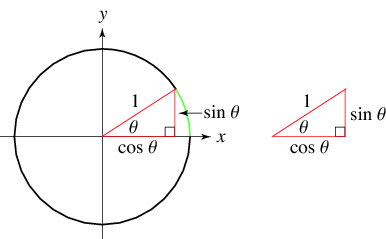
\includegraphics[scale=0.5]{images/01_precalculo/trigonometry.png}
\caption{Trigonometría}
\end{figure}

\begin{figure}[h]
\centering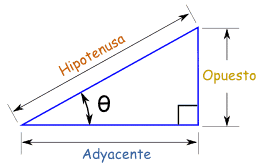
\includegraphics[scale=0.6]{images/01_precalculo/hipotenusa.png}
\caption{Hipotenusa}
\end{figure}

\begin{definition}
Definimos las \textbf{funciones trigonométricas} $\cos(\phi) = x$ y $\sin(\phi) = y$, llamadas coseno de $\phi$ y seno de $\phi$ respectivamente.

En la siguiente figura podemos ver la circunferencia unitaria y un ángulo $\theta$ en verde.  Vemos que queda formado un triángulo rectángulo en rojo.


En términos de un triángulo rectángulo, llamamos \textbf{catetos} a los lados del ángulo rectángulo, e hipotenusa al otro lado.  En términos del ángulo $\phi$ entre la hipotenusa y un cateto, lo llamamos \textbf{cateto adyacente}, y al otro cateto lo llamamos \textbf{cateto opuesto}.

Se verifica entonces

$$\cos(\theta) = \frac{\textrm{Adyacente}}{\textrm{Hipotenusa}}$$

$$\sin(\theta) = \frac{\textrm{Opuesto}}{\textrm{Hipotenusa}}$$

Definimos también las \textbf{funciones trigonométricas} tangente, secante, cosecante y cotangente a continuación, siempre y cuando no se anule el denominador.

$$ \tan(\theta) = \frac{\sin(\theta)}{\cos(\theta)}$$

$$ \sec(\theta) = \frac{1}{\cos(\theta)}$$

$$ \mathrm{cosec}(\theta) = \frac{1}{\sin(\theta)}$$

$$ \cot(\theta) = \frac{1}{\tan(\theta)}$$

\end{definition}

\begin{observation}[Identidad trigonométrica fundamental] \index{Trigonometría!Identidad trigonométrica fundamental}
Para cualquier $\phi \in \mathbb{R}$ se verifica la identidad trigonométrica fundamental:

$$ \cos^2(\phi) + \sin^2(\phi) = 1$$
\end{observation}

\begin{proof}
Dado $\phi \in \RR$, como $x = \cos(\phi)$, $y = \sin(\phi)$ y $(x,y)$ es un punto de la circunferencia unitaria $x^2 + y^2 = 1$, se verifica $\cos^2(\phi) + \sin^2(\phi) = 1$.
\end{proof}



\section{Tabla de ángulos y valores} \index{Trigonometría!Tabla de ángulos y valores}

Puede ser útil conocer los siguientes datos sobre algunos ángulos.

\begin{figure}[h]
\centering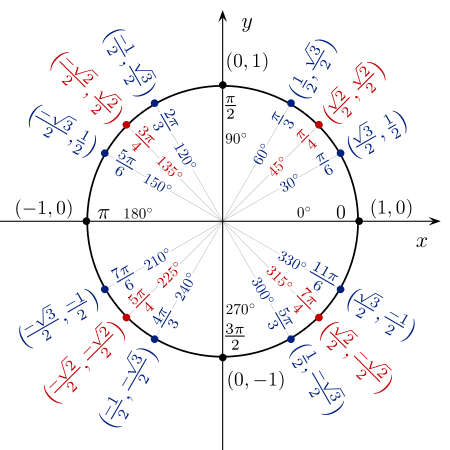
\includegraphics[scale=0.5]{images/01_precalculo/unit_circle_angles_color.png}
\caption{Ángulos en la circunferencia unitaria}
\end{figure}

\begin{center}
  \begin{tabular}{| c | c | c | c | }
    \hline
    Radianes & Grados & Vértice & Aproximado \\ \hline \hline
    $0$ & $0$ & $(1,0)$ & $(1,0)$ \\ 
    $\pi/6$ & $30$ & $(\sqrt{3}, 1)/2$ & $(0.866, 0.5)$ \\
    $\pi/4$ & $45$ & $(\sqrt{2}, \sqrt{2})/2$ & ($0.707, 0.707)$ \\
    $\pi/3$ & $60$ & $(1, \sqrt{3})/2$ & $(0.5, 0.866)$ \\
    $\pi/2$ & $90$ & $(0, 1)$ & $(0, 1)$ \\
    $2\pi/3$ & $120$ & $(-1, \sqrt{3})/2$ & $(-0.5, 0.866)$ \\
    $3\pi/4$ & $135$ & $(-\sqrt{2}, \sqrt{2})/2$ & $(-0.707, 0.707)$ \\
    $5\pi/6$ & $150$ & $(-\sqrt{3}, 1)/2$ & $(-0.866, 0.5)$ \\
    $\pi$ & $180$ & $(-1, 0)$ & $(-1, 0)$ \\
    $7\pi/6$ & $210$ & $(-\sqrt{3}, -1)/2$ & $(-0.866, -0.5)$ \\
    $5\pi/4$ & $225$ & $(-\sqrt{2}, -\sqrt{2})/2$ & $(-0.707, -0.707)$ \\
    $4\pi/3$ & $240$ & $(-1, -\sqrt{3})/2$ & $(-0.5, -0.866)$ \\
    $3\pi/2$ & $270$ & $(0, -1)$ & $(0, -1)$ \\
    $5\pi/3$ & $300$ & $(1, -\sqrt{3})/2$ & $(0.5, -0.866)$ \\
    $7\pi/4$ & $315$ & $(\sqrt{2}, -\sqrt{2})/2$ & $(0.707, -0.707)$ \\
    $11\pi/6$ & $330$ & $(\sqrt{3}, -1)/2$ & $(0.866, -0.5)$ \\
    $2\pi$ & $0$ & $(1,0)$ & $(1,0)$ \\ 

    \hline
  \end{tabular}
\end{center}


\section{Funciones trigonométricas}

\begin{definition}[Seno] \index{Trigonometría!Función $\sin(x)$ }
La \textbf{función seno} es $\sin : \mathbb{R} \to \mathbb{R}$ con 

$$ x \to \sin(x)$$

A continuación la \textbf{gráfica} de la función seno
\end{definition}

\begin{figure}[h]
\centering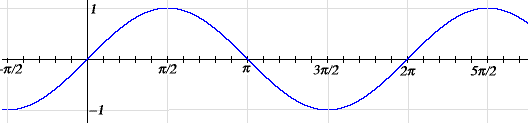
\includegraphics[scale=0.5]{images/01_precalculo/sin.png}
\caption{$\sin(x)$}
\end{figure}

\begin{property}
Algunas propiedades de $\sin(x)$

\begin{itemize}
	
\item Sus \textbf{ceros} son $C_0(f) = \{ k\pi, \textrm{ con } k \in \mathbb{Z} \}$
	
\item Es \textbf{impar}, es decir $\sin(-x) = -\sin(x)$
	
\end{itemize}
\end{property}

\begin{definition}[Coseno] \index{Trigonometría!Función $\cos(x)$ }
La \textbf{función coseno} es $\cos : \mathbb{R} \to \mathbb{R}$ con 

$$ x \to \cos(x)$$

A continuación la gráfica de la función coseno.
\end{definition}

\begin{figure}[h]
\centering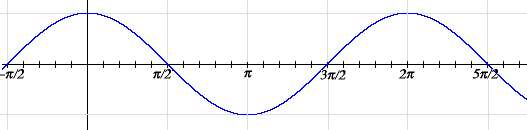
\includegraphics[scale=0.5]{images/01_precalculo/cos.png}
\caption{$\cos(x)$}
\end{figure}

\begin{property}
Algunas propiedades de $\cos(x)$

\begin{itemize}

\item Para todo ángulo se verifica que $\cos(x) = \sin(x + \frac{\pi}{2})$.  Es decir la curva se \textbf{traslada} en $\pi/2$ hacia la izquierda de la gráfica del seno.

\item Sus \textbf{ceros} son 

$$C_0(f) = \{ \frac{\pi}{2} + k\pi, \textrm{ con } k \in \mathbb{Z} \}$$

(son los de la función seno trasladados).

\item Es \textbf{par}, es decir $\cos(x) = \cos(-x)$

\end{itemize}
\end{property}

\begin{property}
Algunas propiedades comunes de $\sin(x)$ y $\cos(x)$

\begin{itemize}
\item La \textbf{imagen} tanto de $\sin(x)$ como de $\cos(x)$ es el intervalo $[-1,1]$.
	
\item Son \textbf{periódicas} con período $2\pi$, es decir $f(x) = f(x + 2\pi)$.  
	
O sea que el gráfico obtenido en el intervalo $[0, 2\pi)$ se repite periódicamente.
	
\item \textbf{No son inyectivas}.
\end{itemize}
\end{property}

\begin{definition}[Tangente] \index{Trigonometría!Función $\tan(x)$ }
La \textbf{función tangente} es $\tan : \mathbb{R} - C_0(\cos(x)) \to \mathbb{R}$, con 

$$ x \to \frac{\sin(x)}{\cos(x)} $$

A continuación su gráfica 
\end{definition}

\begin{figure}[h]
\centering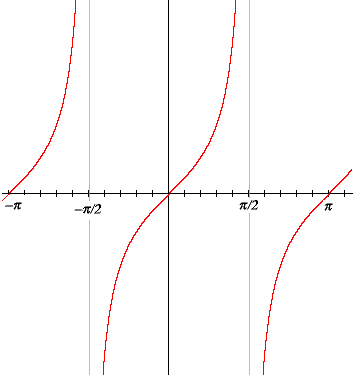
\includegraphics[scale=0.5]{images/01_precalculo/tan.png}
\caption{$\tan(x)$}
\end{figure}

\begin{property}
Algunas propiedades de $\tan(x)$

\begin{itemize}
\item Los \textbf{ceros} de $\tan(x)$ coinciden con los de $\sin(x)$
	
\item Es \textbf{impar}, es decir $\tan(-x) = -\tan(x)$
	
\item Es \textbf{periódica} con período $\pi$.  Es decir $\tan(x) = \tan(x+\pi)$.
	
\item Tiene \textbf{asíntotas verticales} $x = \frac{\pi}{2} + k \pi$ con $k \in \mathbb{Z}$
\end{itemize}
\end{property}

\subsection{Las funciones $\sec(x)$ y $\mathrm{cosec}(x)$ y $\cot(x)$}

\begin{definition}[Secante, cosecante y cotangente] 
La \textbf{función secante} \index{Trigonometría!Función Secante} $\sec : \mathbb{R} - C_0(\sin(x)) \to \mathbb{R}$ con $x \to \frac{1}{\cos(x)} $ 

A continuación su gráfica

La \textbf{función cosecante} \index{Trigonometría!Función Cosecante} $\mathrm{cosec}(x) = \frac{1}{\sin(x)}$ es análoga a la función secante.

La \textbf{función cotangente} \index{Trigonometría!Función Cotangente} es $\cot(x) = \frac{1}{\tan(x)}$.  A continuación su gráfica
\end{definition}

\begin{figure}[h]
\centering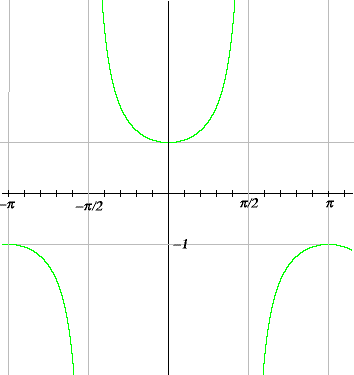
\includegraphics[scale=0.5]{images/01_precalculo/sec.png}
\caption{$\sec(x)$}
\end{figure}

\begin{figure}[h]
\centering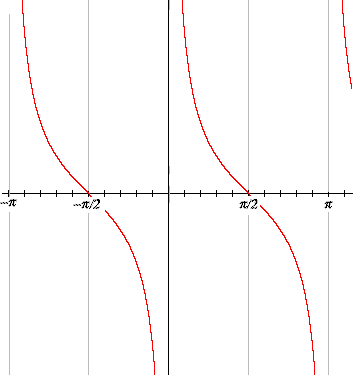
\includegraphics[scale=0.5]{images/01_precalculo/cot.png}
\caption{$\cot(x)$}
\end{figure}


\section{Funciones trigonométricas inversas}

Vimos que las funciones $\sin(x)$, $\cos(x)$ y $\tan(x)$ no son inyectivas.  

Restringiendo el dominio y el codominio podemos obtener una función biyectiva.

\begin{definition}
\begin{itemize}
Definimos las funciones trigonométricas inversas como sigue

\item Restringiendo $\sin(x)$ a $[-\frac{\pi}{2}, \frac{\pi}{2}] \to [-1,1]$ obtenemos una función biyectiva cuya inversa llamamos $ \arcsin(x) $. \index{Trigonometría!Función Arco-seno}

\item Restringiendo $\cos(x)$ a $[0, \pi] \to [-1,1]$ obtenemos una función biyectiva cuya inversa llamamos $ \arccos(x) $. \index{Trigonometría!Función Arco-coseno}

\item Restringiendo $\tan(x)$ a $(-\frac{\pi}{2}, \frac{\pi}{2}) \to \mathbb{R}$ obtenemos una función biyectiva cuya inversa llamamos $\arctan(x)$ \index{Trigonometría!Función Arco-tangente}

\end{itemize}
\end{definition}

\subsection{Ángulo respecto al eje $x$}

En el plano coordenado $\mathbb{R}^2$, es estandard medir ángulos respecto al lado positivo del eje $x$ en sentido antihorario, como muestra la figura

\begin{figure}[h]
\centering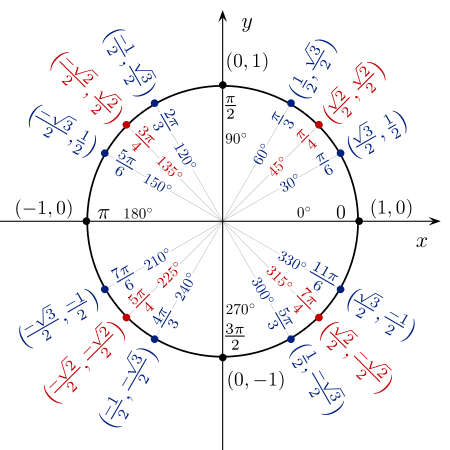
\includegraphics[scale=0.5]{images/01_precalculo/unit_circle_angles_color.png}
\caption{Ángulos en la circunferencia unitaria}
\end{figure}

Supongamos que queremos averiguar el ángulo que forma el vector $v = (-1,-1)$ respecto al eje $x$.  

Como $||v|| = \sqrt{2}$, sabemos que $\cos(\phi) = \sin(\phi) = - \sqrt{2}/2$

Ahora que pasa, la calculadora arroja los siguientes resultados: $\arccos(-\sqrt{2}/2) = 3 \pi/4 $ y $\arcsin(- \sqrt{2}/2) = - \pi / 4$.  

No sólo nos da dos resultados distintos entre sí, sino que ninguno de ellos es el buscado.  Notar que $3\pi/4$ pertenece al segundo cuadrante, $- \pi/4$ pertenece al cuarto cuadrante, y nuestro vector $(-1,-1)$ pertenece al tercer cuadrante.

La idea para obtener el ángulo correcto es analizar el cuadrante que queremos en el dibujo, y considerar ángulos semejantes en el cuadrante en cuestión.  En este caso queremos tercer cuadrante, y lo podemos obtener como $\pi + \pi/4 = 5\pi/4$

Ejercicio: Calcular el ángulo con respecto al eje $x$ de $(- \sqrt{3}, -1)$.  La respuesta es $7\pi/6 = 210^{\circ}$

\section{Función sinusoidal}

\begin{definition}[Función sinusoidal] \index{Función!Ejemplos!Función sinusoidal}
Una función $f$ se dice que es una \textbf{función sinusoidal} si es de la forma $f : \mathbb{R} \to \mathbb{R}$ con 

$$f(x) = K \sin(ax+b)$$

La curva gráfica de la función sinusoidal se llama onda sinusoidal, o sinusoide.  En el gráfico a continuación se representa una sinusoide.

\begin{itemize}
\item La \textbf{amplitud} es $\boxed{ K } $.

\item La \textbf{frecuencia} (ordinaria) es $ \boxed{f = \frac{a}{2\pi} }$ (cíclos por unidad de tiempo).

\item El \textbf{período} es $ \boxed{ \frac{1}{f} }$, el intervalo en que vuelve a empezar

\item La frecuencia angular es $a$.
\item La fase es $b$.
\item El ángulo de fase es $\frac{b}{a}$.  La curva se traslada en esa cantidad.

Si es negativo se retrasa, es decir se corre a la derecha.  Si es positivo se adelanta, es decir se corre a la izquierda.

\end{itemize}

Observar que la función coseno es sinusoidal porque $\cos(x) = \sin(x + \pi/2)$
\end{definition}

\begin{figure}[h]
\centering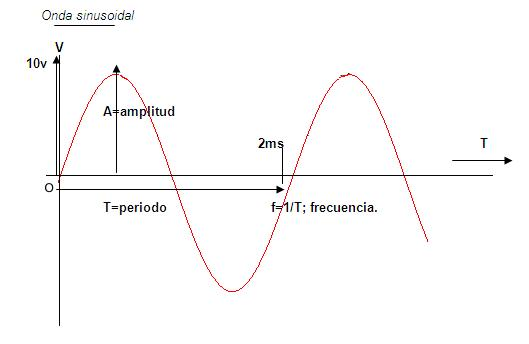
\includegraphics[scale=0.7]{images/01_precalculo/sinusoide.jpg}
\caption{Sinusoide}
\end{figure}

\section{Identidades trigonométricas}

\begin{definition}[Identidad trigonométrica] \index{Trigonometría!Identidad trigonométrica}
Una \textbf{identidad trigonométrica} es una ecuación que se verifican para todo valor del ángulo, por ejemplo la identidad trigonométrica fundamental 

$$ \cos^2(\phi) + \sin^2(\phi) = 1 $$
\end{definition}

\begin{definition}[Fórmula de Euler]
La \textbf{fórmula de Euler} establece que dado $\phi \in \mathbb{R}$, entonces

$$ e^{i \phi} = \cos(\phi) + i \sin(\phi) $$
\end{definition}

\begin{observation}
La exponencial compleja cumple la siguiente propiedad 

$$ e^{i (\alpha + \beta)} = e^{i \alpha} e^{i \beta} $$

Por lo tanto

\begin{eqnarray*} 
	e^{i (\alpha + \beta)} &=& \cos(\alpha + \beta) + i \sin(\alpha + \beta) \\
	&=& [\cos(\alpha) + i \sin(\alpha) ] [\cos(\beta) + i \sin(\beta)] \\
	&=& [\cos(\alpha)\cos(\beta) - \sin(\alpha)\sin(\beta)] + i [\cos(\alpha)\sin(\beta) + \sin(\alpha)\cos(\beta)]
\end{eqnarray*}
	
\end{observation}

\subsection{Suma de ángulos} 

Igualando parte real e imaginaria del número complejo obtenemos fórmulas para el seno y el coseno de la suma de dos ángulos:

\index{Trigonometría!Identidad trigonométrica!$\cos(\alpha + \beta)$ } \index{Trigonometría!Identidad trigonométrica!$\sin(\alpha + \beta)$ }

\begin{eqnarray*}
\cos(\alpha + \beta) &=& \cos(\alpha)\cos(\beta) - \sin(\alpha)\sin(\beta) \\
\sin(\alpha + \beta) &=& \cos(\alpha)\sin(\beta) + \sin(\alpha)\cos(\beta)
\end{eqnarray*}

También podemos verificar dichas identidades geométricamente mediante el siguiente gráfico 

\begin{figure}[h]
\centering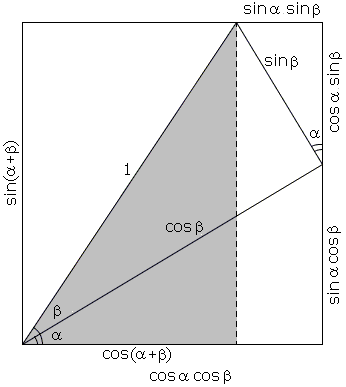
\includegraphics[scale=0.7]{images/01_precalculo/cos_of_sum.png}
\caption{Coseno de la suma}
\end{figure}

Y recordando que $\cos(x)$ es par, y $\sin(x)$ es impar, obtenemos fórmulas para el seno y el coseno de la diferencia de dos ángulos:

\index{Trigonometría!Identidad trigonométrica!$\cos(\alpha - \beta)$ } \index{Trigonometría!Identidad trigonométrica!$\sin(\alpha - \beta)$ }

\begin{eqnarray*}
\cos(\alpha - \beta) &=& \cos(\alpha)\cos(\beta) + \sin(\alpha)\sin(\beta) \\
\sin(\alpha - \beta) &=& \sin(\alpha)\cos(\beta) -\cos(\alpha)\sin(\beta)
\end{eqnarray*}

Además, para la tangente de la suma de dos ángulos obtenemos

\index{Trigonometría!Identidad trigonométrica!$\tan(\alpha + \beta)$ } 

\begin{eqnarray*}
\tan(\alpha + \beta) &=& \frac{\sin(\alpha + \beta)}{\cos(\alpha + \beta)} \\
 &=& \frac{\cos(\alpha)\sin(\beta) + \sin(\alpha)\cos(\beta)}{\cos(\alpha)\cos(\beta) - \sin(\alpha)\sin(\beta)} \\
 &=& \frac{\frac{\cos(\alpha)\sin(\beta)}{\cos(\alpha)\cos(\beta)} + \frac{\sin(\alpha)\cos(\beta)}{\cos(\alpha)\cos(\beta)}}{\frac{\cos(\alpha)\cos(\beta)}{\cos(\alpha)\cos(\beta)} - \frac{\sin(\alpha)\sin(\beta)}{\cos(\alpha)\cos(\beta)}} \\
 &=& \frac{\tan(\beta) + \tan(\alpha)}{1 - \tan(\alpha)\tan(\beta)}
\end{eqnarray*}

\subsection{Suma de senos y de cosenos}

Se verifica entonces que

\begin{eqnarray*}
\cos(\alpha + \beta) + \cos(\alpha - \beta) &=& 2 \cos(\alpha)\cos(\beta) \\
\cos(\alpha + \beta) - \cos(\alpha - \beta) &=& -2 \sin(\alpha) \sin(\beta) \\
\sin(\alpha + \beta) + \sin(\alpha - \beta) &=& 2 \sin(\alpha) \cos(\beta) \\
\sin(\alpha + \beta) - \sin(\alpha - \beta) &=& 2 \cos(\alpha) \sin(\beta) 
\end{eqnarray*}

Si $a = \alpha + \beta$ y $b = \alpha - \beta$, se tiene que $\alpha = \frac{a+b}{2}$ y $\beta = \frac{a-b}{2}$, y 

\index{Trigonometría!Identidad trigonométrica!$\cos(a) + \cos(b)$} 
\index{Trigonometría!Identidad trigonométrica!$\cos(a) - \cos(b)$} 
\index{Trigonometría!Identidad trigonométrica!$\sin(a) + \sin(b)$} 
\index{Trigonometría!Identidad trigonométrica!$\sin(a) - \sin(b)$} 

\begin{eqnarray*}
\cos(a) + \cos(b) &=& 2 \cos(\frac{a+b}{2})\cos(\frac{a-b}{2}) \\
\cos(a) - \cos(b) &=& -2 \sin(\frac{a+b}{2})\sin(\frac{a-b}{2}) \\
\sin(a) + \sin(b) &=& 2 \sin(\frac{a+b}{2}) \cos(\frac{a-b}{2}) \\
\sin(a) - \sin(b) &=& 2 \cos(\frac{a+b}{2}) \sin(\frac{a-b}{2}) 
\end{eqnarray*}

\subsection{Algo extra...}

Usando la fórmula de Euler, y que coseno es par y seno es par

\begin{eqnarray*}
e^{i \alpha} &=& \cos(\alpha) + i \sin(\alpha) \\
e^{- i \alpha} &=& \cos(\alpha) - i \sin(\alpha)
\end{eqnarray*}

Sumando y restando respectivamente

\begin{eqnarray*}
e^{i \alpha} + e^{-i \alpha} &=& 2 \cos(\alpha) \\
e^{i \alpha} - e^{-i \alpha} &=& 2 i \sin(\alpha)
\end{eqnarray*}

Por lo tanto

\begin{eqnarray*}
\cos(\alpha) &=& \frac{e^{i \alpha} + e^{-i \alpha}}{2} \\
\sin(\alpha) &=& \frac{e^{i \alpha} - e^{-i \alpha}}{2i}
\end{eqnarray*}

\section{Pendiente de una recta} \index{Trigonometría!Pendiente de una recta}

\begin{observation}[Pendiente de una recta]
La \textbf{ecuación cartesiana} de una recta $R$ en el plano es de la forma

$$ y = mx + b$$

Decimos que $m$ es la \textbf{pendiente} de la recta, y que $b$ es la \textbf{ordenada al origen}.

Entonces la pendiente $m$ de la recta $R$ es igual a la tangente del ángulo $\phi$ entre el eje $x$ y la recta dada.
\end{observation}

\begin{figure}[h]
\centering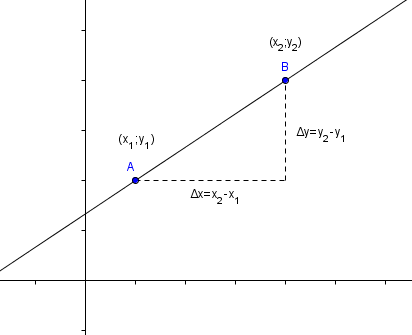
\includegraphics[scale=1]{images/01_precalculo/pendiente_recta.png}
\caption{Pendiente de una recta}
\end{figure}

\begin{proof}
Supongamos que sólo conocemos dos puntos de la recta $(x_1, y_1)$ y $(x_2, y_2)$, con $x_1 \neq x_2$, como se muestra en la siguiente figura, y que queremos encontrar la ecuación cartesiana de la recta.

Se tiene que una \textbf{ecuación paramétrica} de la recta $R$ es

$$(x,y) = (x_1, y_1) + \lambda(x_2 - x_1, y_2 - y_1)$$

con $\lambda \in \mathbb{R}$.  O sea que

\begin{eqnarray*}
x &=& x_1 + \lambda (x_2 - x_1) \\
y &=& y_1 + \lambda (y_2 - y_1) 
\end{eqnarray*}

De la primera ecuación

$$ \lambda = \frac{x - x_1}{x_2 - x_1}$$

En la segunda, y llamando $\triangle x = x_2 - x_1$ y $\triangle y = y_2 - y_1$

\begin{eqnarray*}
y &=& y_1 + \frac{x - x_1}{x_2 - x_1} (y_2 - y_1) \\
y &=& \frac{\triangle y}{\triangle x} x + \left( y_1 - x_1 \frac{\triangle y}{\triangle x} \right)
\end{eqnarray*}

Finalmente encontramos la ecuación cartesiana de la recta

$$ y = mx + b $$

donde $m = \frac{\triangle y}{\triangle x}$ y $ b = \left( y_1 - x_1 \frac{\triangle y}{\triangle x} \right) $

Notar que también podemos escribir esta ecuación como

$$ y - y_1 = m (x - x_1) $$

Volviendo a ver el dibujo, observamos que podemos formar un triángulo rectángulo donde $\triangle x$ y $\triangle y$ son sus catetos.  Considerando el ángulo $\alpha$ entre la recta $y = y_1$ y la recta dada, vemos que $m = \frac{\triangle y}{ \triangle x} = \tan(\alpha)$, pues es el cociente del cateto opuesto con el cateto adyacente.

Es decir que la pendiente de la recta es igual a la tangente del ángulo $\alpha$ entre la recta $R$ y la recta horizontal $y = y_1$.  O lo que es lo mismo, entre la recta $R$ y el eje $x$ (es el mismo ángulo $\alpha$).

\end{proof}

\section{Teoremas del seno y del coseno}

\begin{theorem}[Teorema del Seno] \label{teorema_del_seno}

Sea $ABC$ un triángulo, llamamos $\alpha, \beta, \gamma$ a sus ángulos, y $a,b,c$ a sus lados opuestos.

Entonces,

$$ \boxed{ \frac{a}{\sin(\alpha)} = \frac{b}{\sin(\beta)} = \frac{c}{\sin(\gamma)} } $$

\end{theorem}

\begin{figure}[h]
\centering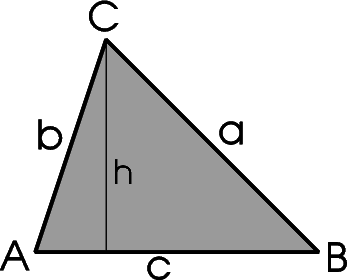
\includegraphics[scale=0.4]{images/01_precalculo/teorema_seno.png}
\caption{Teorema del seno}
\end{figure}

\begin{proof}
Si $h = b \sin(\alpha)$ es la altura desde el vértice $C$, entonces el área del triángulo es $A = \frac{ch}{2} = \frac{c b \sin(\alpha)}{2}$

Similarmente, trazando la altura desde los otros vértices obtenemos $A = \frac{ac \sin(\beta)}{2} = \frac{ab \sin(\gamma)}{2}$, es decir

$$ 2A = bc \sin(\alpha) = ac \sin(\beta) = ab \sin(\gamma) $$

dividiendo por $abc$

$$ \frac{2A}{abc} = \frac{\sin(\alpha)}{a} = \frac{\sin(\beta)}{b} = \frac{\sin(\gamma)}{c} $$

tomando el recíproco

$$ \frac{abc}{2A} = \frac{a}{\sin(\alpha)} = \frac{b}{\sin(\beta)} = \frac{c}{\sin(\gamma)} $$
\end{proof}

\begin{proof}
Ahora vamos a dar otra demostración, suponiendo que el triángulo es agudo.

Primero partimos el triángulo en dos triángulos rectángulos, trazando la altura $h$ desde el vértice $C$, como en la figura siguiente


Luego,

$$ h = b \sin(\alpha) = a \sin(\beta) $$

de donde

$$ \frac{a}{\sin(\alpha)} = \frac{b}{\sin(\beta)} $$

Si trazamos la altura desde el vértice $B$ obtenemos

$$ \frac{a}{\sin(\alpha)} = \frac{c}{\sin(\gamma)} $$

Finalmente

$$ \frac{a}{\sin(\alpha)} = \frac{b}{\sin(\beta)} = \frac{c}{\sin(\gamma)}$$

\end{proof}

\begin{theorem}[Teorema del Coseno] \label{teorema_del_coseno}

Sea $ABC$ un triángulo, llamamos $\alpha, \beta, \gamma$ a sus ángulos, y $a,b,c$ a sus lados opuestos.

Entonces,

$$ \boxed{a^2 = b^2 + c^2 - 2bc \cos(\alpha)} $$

y vale simétricamente para los otros lados, es decir

\begin{eqnarray*}
a^2 &=& b^2 + c^2 - 2bc \cos(\alpha) \\
b^2 &=& a^2 + c^2 - 2ac \cos(\beta) \\
c^2 &=& a^2 + b^2 - 2ab \cos(\gamma)
\end{eqnarray*}
\end{theorem}

\begin{figure}[h]
\centering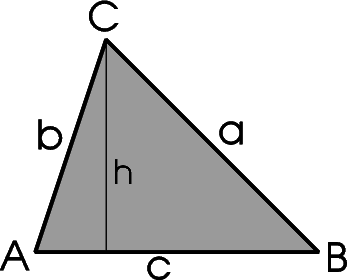
\includegraphics[scale=0.4]{images/01_precalculo/teorema_seno.png}
\caption{Teorema del coseno}
\end{figure}

Observación: En el caso particular de que el triángulo sea rectángulo nos queda el teorema de Pitágoras.  Es decir este teorema es una generalización del teorema de Pitágoras.

\begin{proof}  Demostramos utilizando producto interno.

Situamos el vértice de ángulo $\alpha$ en el origen del plano euclídeo.  Los lados $b$ y $c$ los interpretamos como vectores de $\mathbb{R}^2$, y al lado $a$ como el vector $c-b$.  Luego

$ ||a||^2 = || c-b ||^2 = (c-b) \cdot (c-b) = c^2 - 2bc + b^2 = ||c||^2 + ||b||^2 - 2 ||b|| ||c|| \cos(\alpha) $

Es decir que

$$a^2 = b^2 + c^2 - 2 bc \cos(\alpha)$$

\end{proof}

\begin{proof}  Demostramos utilizando distancia euclídea.
	
Dispongamos sus vértices en el plano cartesiano de la siguiente manera

$A = (0,0)$, $B = (b, 0)$ y $C = (a \cos(\alpha), a \sin(\alpha))$

La distancia entre $B$ y $C$ es 

$$ d(B,C) = c = \sqrt{(a \cos(\alpha) - b)^2 + (a \sin(\alpha) - 0)^2 } $$

Por lo tanto

$$ c^2 = a^2 \cos^2(\alpha) - 2ab \cos(\alpha) + b^2 + a^2 \sin^2(\alpha)$$

$$ c^2 = a^2 + b^2 - 2ab \cos(\alpha) $$

Rotando la forma en la que ubicamos los vértices del triángulo sobre el plano, obtenemos las otras identidades.

\end{proof}

\begin{proof}
Ahora vamos a dar otra demostración, suponiendo que el triángulo es agudo.  Como antes trazamos la altura desde el vértice $C$.  Llamamos $H$ al punto del lado $AB$ donde que se intersecta con dicha altura.

Luego $AH = b \cos(\alpha) $ y $HB = c - AH = c - b \cos(\alpha)$

Por Pitágoras en el triángulo rectángulo $AHC$

$$ b^2 = AH^2 + h^2 $$

y por Pitágoras en el triángulo rectángulo $CHB$

$$ a^2 = h^2 + HB^2 $$

restando

$$b^2 - a^2 = AH^2 - HB^2 $$

reemplazando $HB$ y $AH$

$$b^2 - a^2 = b^2 \cos^2(\alpha) - (c - b \cos(\alpha))^2 $$

$$b^2 - a^2 = b^2 \cos^2(\alpha) - (c^2 - 2bc \cos(\alpha) + b^2 \cos^2(\alpha)) $$

$$b^2 - a^2 = b^2 \cos^2(\alpha) - (c^2 - 2bc \cos(\alpha) + b^2 \cos^2(\alpha)) $$

$$b^2 - a^2 = - c^2 + 2bc \cos(\alpha) $$

$$ a^2 = b^2 + c^2 - 2bc \cos(\alpha) $$
\end{proof}



\chapter{Física}

\begin{definition}
Llamamos \textbf{Espacio Euclídeo} al conjunto $\mathbb{R}^n$, a sus elementos los llamamos \textbf{vectores} \index{Física!Vectores}, y llamamos \textbf{escalares} a los elementos de $\mathbb{R}$.

Están definidas las operaciones suma de vectores, y multiplicación de un vector por un escalar, como definimos a continuación.

Sea $u,v \in \mathbb{R}^n$ y $k \in \mathbb{R}$, digamos $u = (u_1, u_2, \ldots, u_n)$ y $v = (v_1, v_2, \ldots, v_n)$.

Entonces la \textbf{suma de vectores} \index{Física!Vectores!Suma} la definimos como

$$ u + v = (u_1 + v_1, u_2 + v_2, \ldots, u_n + v_n) $$

y definimos el \textbf{producto de un vector por un escalar} \index{Física!Vectores!Producto con un escalar} como

$$ ku = (k u_1, k u_2, \ldots, k u_n) $$

También está definido el \textbf{producto escalar} \index{Física!Vectores!Producto escalar} (o producto interno estándard) entre dos vectores $u$ y $v$ como

$$ u \cdot v = \sum_{i=1}^n u_i v_i = u_1 v_1 + u_2 v_2 + \ldots + u_n v_n $$

Dos vectores $u$ y $v$ se dicen \textbf{ortogonales} \index{Física!Vectores!Ortogonales} sii $u \cdot v = 0$

Definimos la \textbf{norma} \index{Física!Vectores!Norma} del vector $u$ como

$$ |u| = \sqrt{u \cdot u} = \sqrt{u_1^2 + u_2^2 + \ldots + u_n^2}$$

Si $|u| = 1$ decimos que $u$ es un \textbf{versor} \index{Física!Vectores!Versor}.  Dado $v \in \mathbb{R}^n$, $v \neq 0$, llamamos \textbf{versor asociado} a $v$ al versor $v / |v|$

El \textbf{ángulo entre dos vectores} \index{Física!Vectores!Ángulo} $u$ y $v$ (no nulos) lo definimos como $ 0 \leq \phi \leq \pi $ tal que

$$ \cos(\phi) = \frac{u \cdot v}{||u|| ||v||}$$

Esto en realidad se deduce del teorema del coseno (Ver \ref{teorema_del_coseno}) de la siguiente manera.

Sea $ABC$ un triángulo, llamamos $\alpha, \beta, \gamma$ a sus ángulos, y $a,b,c$ a sus lados opuestos.

Llamamos también $u = \vec{AC}$ e $v = \vec{AB}$

Entonces, por el teorema del coseno

$$ \boxed{a^2 = b^2 + c^2 - 2bc \cos(\alpha)} $$

Por un lado $a^2 = || u-v ||^2 = \sum_{i=1}^n (u_i - v_i)^2 = \sum_i u_i^2 - 2 \sum_i u_i v_i + \sum_i v_i^2$

Por otro lado $b^2 + c^2 - 2bc \cos(\alpha) = \sum_i u_i^2 + \sum_i v_i^2 - 2 \sqrt{ \sum_i u_i^2 } \sqrt{ \sum_i v_i^2 } \cos(\phi)$

Igualando

$\sum_i u_i^2 - 2 \sum_i u_i v_i + \sum_i v_i^2 = \sum_i u_i^2 + \sum_i v_i^2 - 2 \sqrt{ \sum_i u_i^2 } \sqrt{ \sum_i v_i^2 } \cos(\phi)$

Cancelando

$$ \sum_i u_i v_i = \sqrt{ \sum_i u_i^2 } \sqrt{ \sum_i v_i^2 } \cos(\phi)$$

O sea

$$ u \cdot v = ||u|| ||v|| \cos(\phi)$$

\end{definition}

\begin{figure}[h]
\centering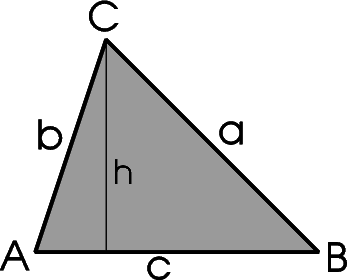
\includegraphics[scale=0.4]{images/01_precalculo/teorema_seno.png}
\caption{Triángulo}
\end{figure}

\begin{observation}
Si $u$ y $v$ no nulos son ortogonales, entonces el ángulo entre ellos es $\pi/2 = 90^{\circ}$
\end{observation}

\begin{definition}[Proyección] \index{Física!Vectores!Proyección}
Si $A$ y $B$ son vectores, la \textbf{proyección} de $A$ sobre $B \neq 0$ es el vector que representamos en la siguiente figura

y se calcula como

$$ proy_B(A) = \frac{A \cdot B}{||B||} \frac{B}{||B||}$$

\end{definition}

\begin{figure}[h]
\centering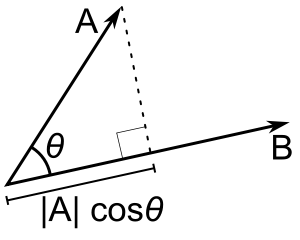
\includegraphics[scale=0.5]{images/01_precalculo/proyeccion_vector.png}
\caption{Proyección de un vector}
\end{figure}

\begin{proof}
Como $ A \cdot B = ||A|| \cdot ||B|| \cos(\theta)$, la norma de la proyección es $||A|| \cos(\theta) = \frac{A \cdot B}{||B||} $, y multiplicando por el versor asociado a $B$, es decir $\frac{B}{||B||}$, obtenemos el vector buscado $proy_B(A) = \frac{A \cdot B}{||B||} \frac{B}{||B||}$.
\end{proof}

\section{Sistema de fuerzas} \index{Física!Sistema de fuerzas}

En física, una \textbf{fuerza} es una acción capaz de imponer una aceleración sobre un cuerpo material.  Se representa mediante un vector. 

Recordemos las tres leyes del movimiento de \textbf{Newton}.

\begin{itemize}
\item La \textbf{primera ley de Newton} establece que todo cuerpo permanece en reposo o movimiento uniforme en linea recta, a menos que una fuerza actúe sobre él.

\item La \textbf{segunda ley de Newton} establece que la aceleración de un cuerpo de masa $m$ es igual a la fuerza resultante que actúa sobre el, dividido su masa, es decir

$$ a = \frac{F}{m} $$

dicho de otra forma

$$F = m \cdot a$$

Su unidad de medida es el Newton, $1 \ N = 1 \ \frac{kg \cdot m}{s^2} $

\item La \textbf{tercera ley de Newton} establece que si un cuerpo $A$ ejerce una fuerza $F_{A/B}$ sobre $B$, entonces $B$ ejerce una fuerza de igual magnitud y sentido contrario $F_{B/A}$ sobre $A$, es decir

$$ F_{A/B} = - F_{B/A} $$

\end{itemize}

Llamamos \textbf{sistema de fuerzas} al conjunto de fuerzas $F_1, F_2, \ldots, F_n$ que actúan sobre un cuerpo.

La \textbf{fuerza resultante} \index{Física!Sistema de fuerzas!Resultante} es $F_r = \sum_{i=1}^n F_i $, y la \textbf{fuerza equilibrante} \index{Física!Sistema de fuerzas!Equilibrante} es $F_e = - F_r$

En el plano, una fuerza $F = (x,y)N$ también la podemos representar como $F = (n,\alpha)$ donde $n = ||F||$ y $\alpha$ es el ángulo del vector $F$ con el eje $x$.

\section{Cinemática} \index{Física!Cinemática}

La \textbf{cinemática} es la parte de la física que estudia el \textbf{movimiento} de los cuerpos, abstrayendose de las causas que lo producen.  Los problemas que resuelve la cinemática son sobre calcular posición, velocidad y aceleración de un cuerpo.

El cuerpo vamos a modelarlo matemáticamente como un punto en el espacio, como si fuera un \textbf{partícula} puntual.

Para determinar su posición primero debemos fijar un \textbf{sistema de referencia}.  Es decir fijar un sistema de coordenadas ortogonales en el plano o el espacio.

De aquí en adelante sólo trabajaremos con partículas que se mueven sobre un plano que representaremos por $\mathbb{R}^2$.

La posición de una partícula queda entonces determinada por el \textbf{vector posición} $r$.

La \textbf{trayectoria} \index{Física!Cinemática!Trayectoria} que sigue una partícula es la función que determina el vector posición en función del tiempo, es decir determina la posición de la partícula en cada instante.

$$ \vec{x}(t) = (x_x(t), x_y(t))$$

En la siguiente figura representamos una trayectoria en el plano

\begin{figure}[h]
\centering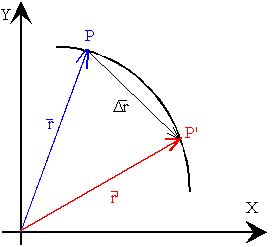
\includegraphics[scale=0.5]{images/01_precalculo/desplazamiento.png}
\caption{Desplazamiento}
\end{figure}

Supongamos que consideramos un intervalo de tiempo $\triangle t = t_f - t_i$.  La \textbf{posición inicial} es $ x_i = x(t_i)$ y la \textbf{posición final} es $x_f = x(t_f)$.  Entonces

\begin{itemize}
\item El \textbf{desplazamiento} es 

$$\triangle x = x(t_f) - x(t_i)$$  

\item La \textbf{distancia recorrida} es $||\triangle x||$

\item La \textbf{velocidad media} es $ v_m = \frac{\triangle x}{ \triangle t} = \frac{x(t_f) - x(t_i)}{\triangle t}$

\item La \textbf{velocidad instantánea} es 

$$ v(t) = \lim_{\triangle t \to 0} \frac{x(t + \triangle t) - x(t)}{\triangle t}$$

\item La \textbf{aceleración media} es $ a_m = \frac{\triangle v}{ \triangle t} = \frac{v(t_f) - v(t_i)}{\triangle t}$

\item La \textbf{aceleración instantánea} es 

$$ a(t) = \lim_{\triangle t \to 0} \frac{v(t+\triangle t) - v(t)}{\triangle t}$$

\end{itemize}

\subsection{Movimiento rectilíneo uniforme (MRU)}

La trayectoria se dice que está en \textbf{movimiento uniforme} también conocido como \textbf{movimiento rectilíneo uniforme} (MRU) \index{Física!Cinemática!MRU} cuando se puede expresar como

$$ x(t) = x_i + v (t - t_i) $$

donde $x_i \in \mathbb{R}^n$ es la posición inicial, es decir $x_i = x(t_i)$, y $v \in \mathbb{R}^n$ es la velocidad (constante).

En este caso, la partícula se mueve sobre una recta a velocidad constante.  La aceleración es nula en todo momento.

\subsection{Movimiento uniformemente variado (MPUV, MRUV)}

La trayectoria se dice que está en \textbf{movimiento uniformemente acelerado} también conocido como \textbf{movimiento uniformemente variado} (MUV) \index{Física!Cinemática!MUV} cuando se puede expresar como

$$ x(t) = x_i + v_i (t-t_i) + \frac{1}{2}a (t-t_i)^2 $$

Donde $x_i \in \mathbb{R}^n$ es la posición inicial, es decir $x_i = x(t_i)$, además $v_i \in \mathbb{R}^n$ es la velocidad inicial, es decir $v_i = v(t_i)$, y $a \in \mathbb{R}^n$ es la aceleración (constante).

La velocidad resulta entonces

$$ v(t) = v_i + a(t-t_i) $$

El MUV lo podemos clasificar según si es rectilíneo o no:

\begin{itemize}
\item Cuando la velocidad inicial $v_i$ es un vector paralelo a la aceleración $a$, la partícula se mueve sobre una recta, y se dice la trayectoria está en \textbf{movimiento rectilíneo uniformemente variado} (MRUV) \index{Física!Cinemática!MRUV}.  

Por ejemplo el tiro vertical (ver \ref{tiro_oblicuo}) es un MRUV.

\item En caso contrario, cuando el vector velocidad inicial $v_i$ no es paralelo al vector aceleración $a$, la partícula se mueve sobre una parábola, y se dice que la trayectoria está en \textbf{movimiento parabólico uniformemente variado} (MPUV) \index{Física!Cinemática!MPUV}.  

Por ejemplo el tiro oblicuo (ver \ref{tiro_oblicuo}) es un MPUV.
\end{itemize}

\subsection{Caída de cuerpos (Tiro oblicuo y vertical)}

La fuerza de gravedad atrae los cuerpos hacia la tierra con una aceleración con intensidad de 

$$ |g| = 9.8 \frac{m}{s^2}$$

Se denomina \textbf{proyectil} todo cuerpo que se mueve sólamente sujeto a una velocidad inicial, y a la fuerza que ejerce su propio peso por la acción de la gravedad, sin considerar otras fuerzas como la resistencia del aire.

Es decir que su trayectoria se puede expresar como

$$ x(t) = x_i + v_i (t-t_i) + \frac{1}{2} g (t-t_i)^2 $$

con $x_i = (x_i, y_i)$ la posición cuando $t= t_i$, $v_i = (v_x,v_y)$ la velocidad cuando $t=t_i$, y $g = (0, -9.8)$.

Si el ángulo entre $v_i$ y la horizontal es de $90^{\circ}$ decimos que es \textbf{tiro vertical} \label{tiro_vertical} \index{Física!Cinemática!Tiro vertical}.  Sinó decimos que es \textbf{tiro oblicuo} \label{tiro_oblicuo}. \index{Física!Cinemática!Tiro oblicuo}

\begin{example}
Si lanzamos un proyectil con $||v_i|| = 400 m/s$ y un ángulo de elevación de $30^{\circ}$.  Considerando $g = 10 m/s^2$.

Entonces la velocidad inicial es

\begin{eqnarray*}
v_i &=& 400 ( \cos(30^{\circ}), \sin(30^{\circ})) \\
 &=& 400 ( \frac{\sqrt{3}}{2}, \frac{1}{2}) \\
 &=& 200 ( \sqrt{3}, 1) \\
 &=& ( 200 \sqrt{3}, 200) 
\end{eqnarray*}

Digamos que la posición inicial es $x_i = (0,0)$.  Luego tenemos que la trayectoria es

$$ x(t) = (0,0) + ( 200 \sqrt{3}, 200) t + \frac{1}{2} (0, -10) t^2 $$

y su velocidad

$$ v(t) = (200\sqrt{3}, 200) + (0, -10) t $$

Luego, a los 5 segundos está en $x(5) = (1000 \sqrt{3}, 875)$

La velocidad a los 5 segundos es $v(5) = (200 \sqrt{3}, 150)$

Se encontrará a 1000 metros de altura cuando

$$ 200 t - 5 t^2 = 1000 $$

Es decir cuando $t_1 = 20 - 10\sqrt{2} \approx 5.85786 $ y tambien cuando $t_2 = 20 + 10\sqrt{2} \approx 34.1421$

La altura máxima alcanzada por el proyectil es cuando $v_y = 0$ es decir

$$ 200 - 10t = 0 $$

O sea cuando $t = 20$, y la altura alcanzada es $x_y(20) = 2000$, en ese instante tiene un velocidad de $v(20) = (200 \sqrt{3}, 0)$

El alcance máximo ocurre cuando $x_y(t) = 0$ es decir cuando

$$ 200 t - 5t^2 = 0 $$

O sea, cuando $t = 0$ está en el punto inicial, el otro es $t = 40$.  Dicho alcance es $x_x(40) = 8000 \sqrt{3}$.  La velocidad con la que llega es $v(40) = (200 \sqrt{3}, -200)$
\end{example}


\appendix
%    Include appendix "chapters" here.
%\include{}

\backmatter
%    Bibliography styles amsplain or harvard are also acceptable.
\bibliographystyle{amsalpha}
\bibliography{}
%    See note above about multiple indexes.
\printindex

\end{document}

%-----------------------------------------------------------------------
% End of amsbook-template.tex
%-----------------------------------------------------------------------